\subsection*{Feature checks between Monte Carlo and ATLAS data}
The figures below are made smaller to reduce the amount of pages. Note that the legend for each figure is 
the same, thus, for rerence on the legend, see figure \ref{fig:MC_Data_comp} in subsection \ref{sec:mcdatacomp} 
on Monte Carlo and ATLAS data comparison.
\begin{figure}
    \centering
    \begin{subfigure}{.49\textwidth}
        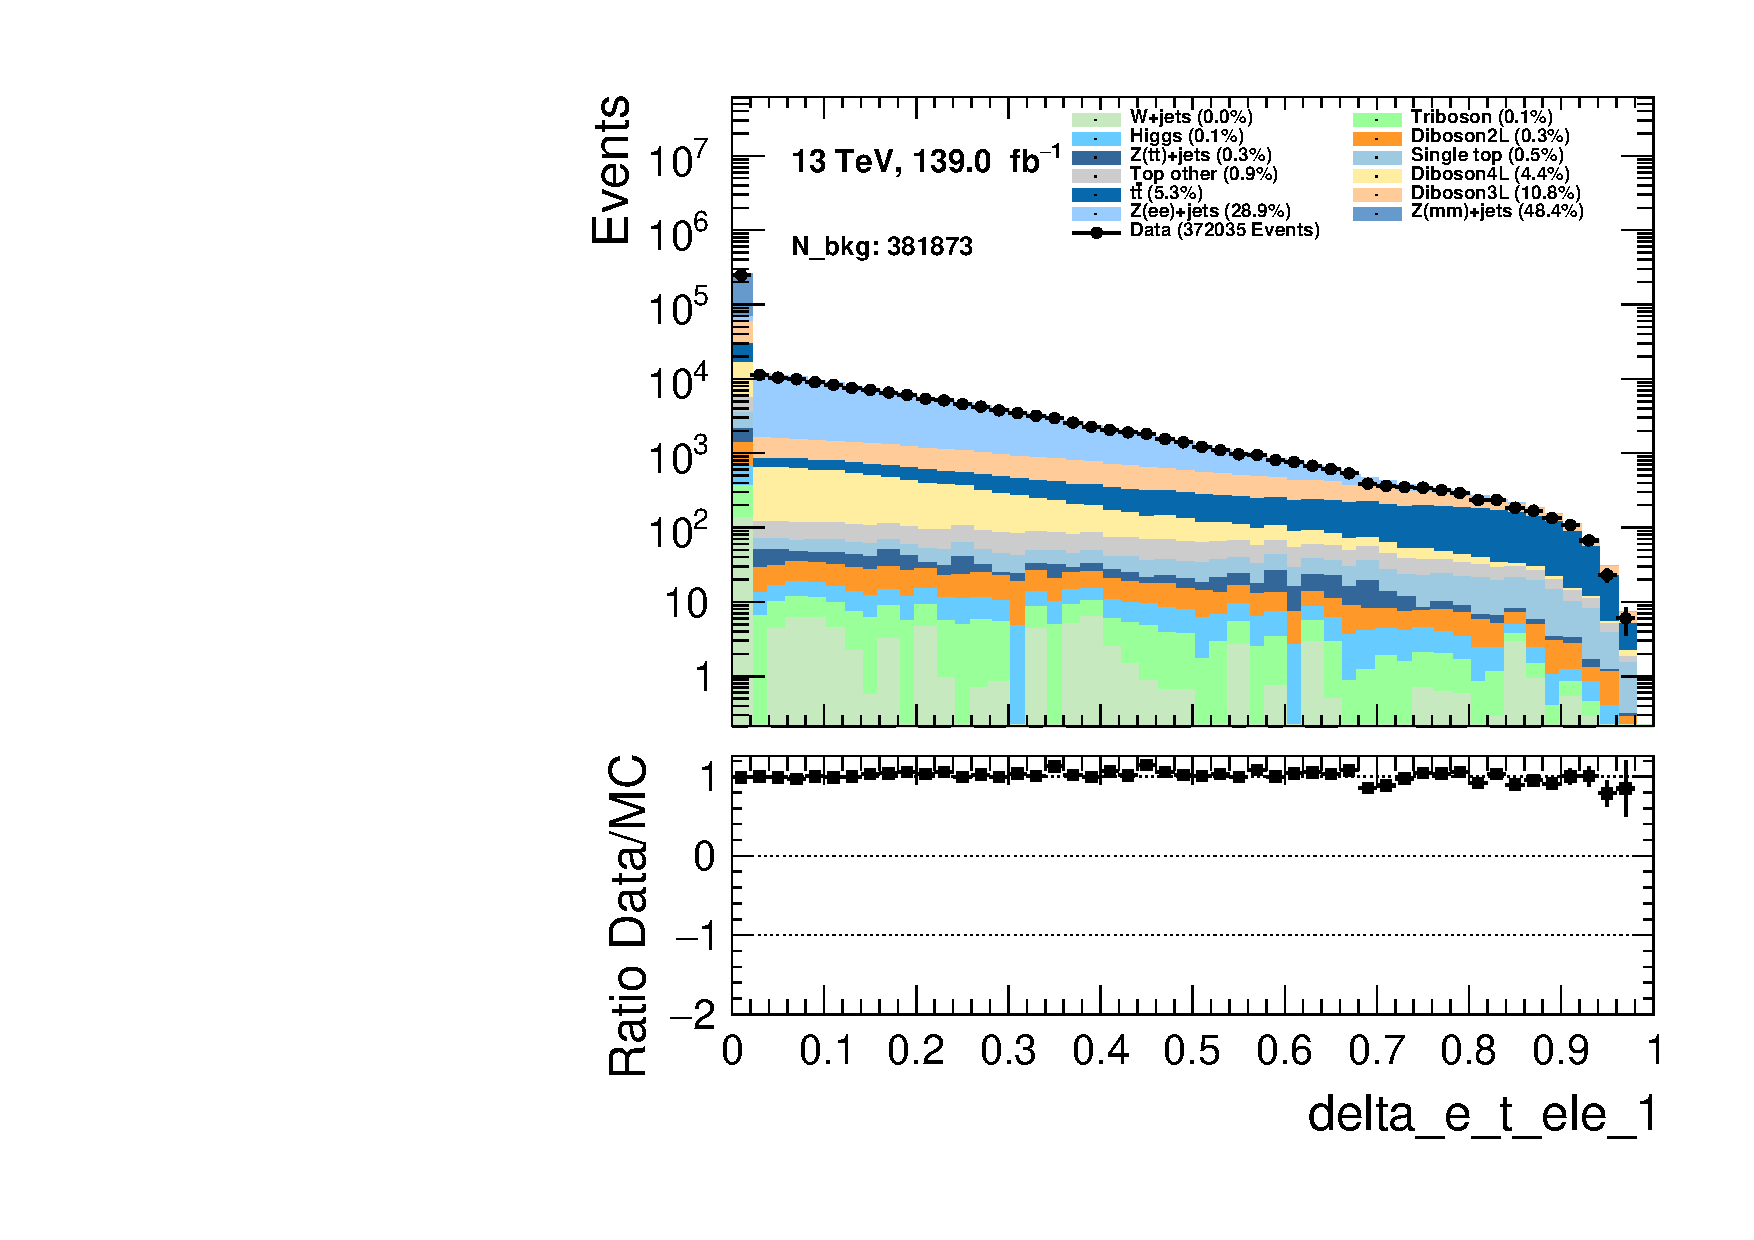
\includegraphics[width=\textwidth]{Figures/MC_Data_comp/delta_e_t_ele_1.pdf}
        \caption{Transverse energy imbalance for the second electron.}
        \label{fig:delta_e_t_ele_1}
    \end{subfigure}
    \hfill
    \begin{subfigure}{.49\textwidth}
        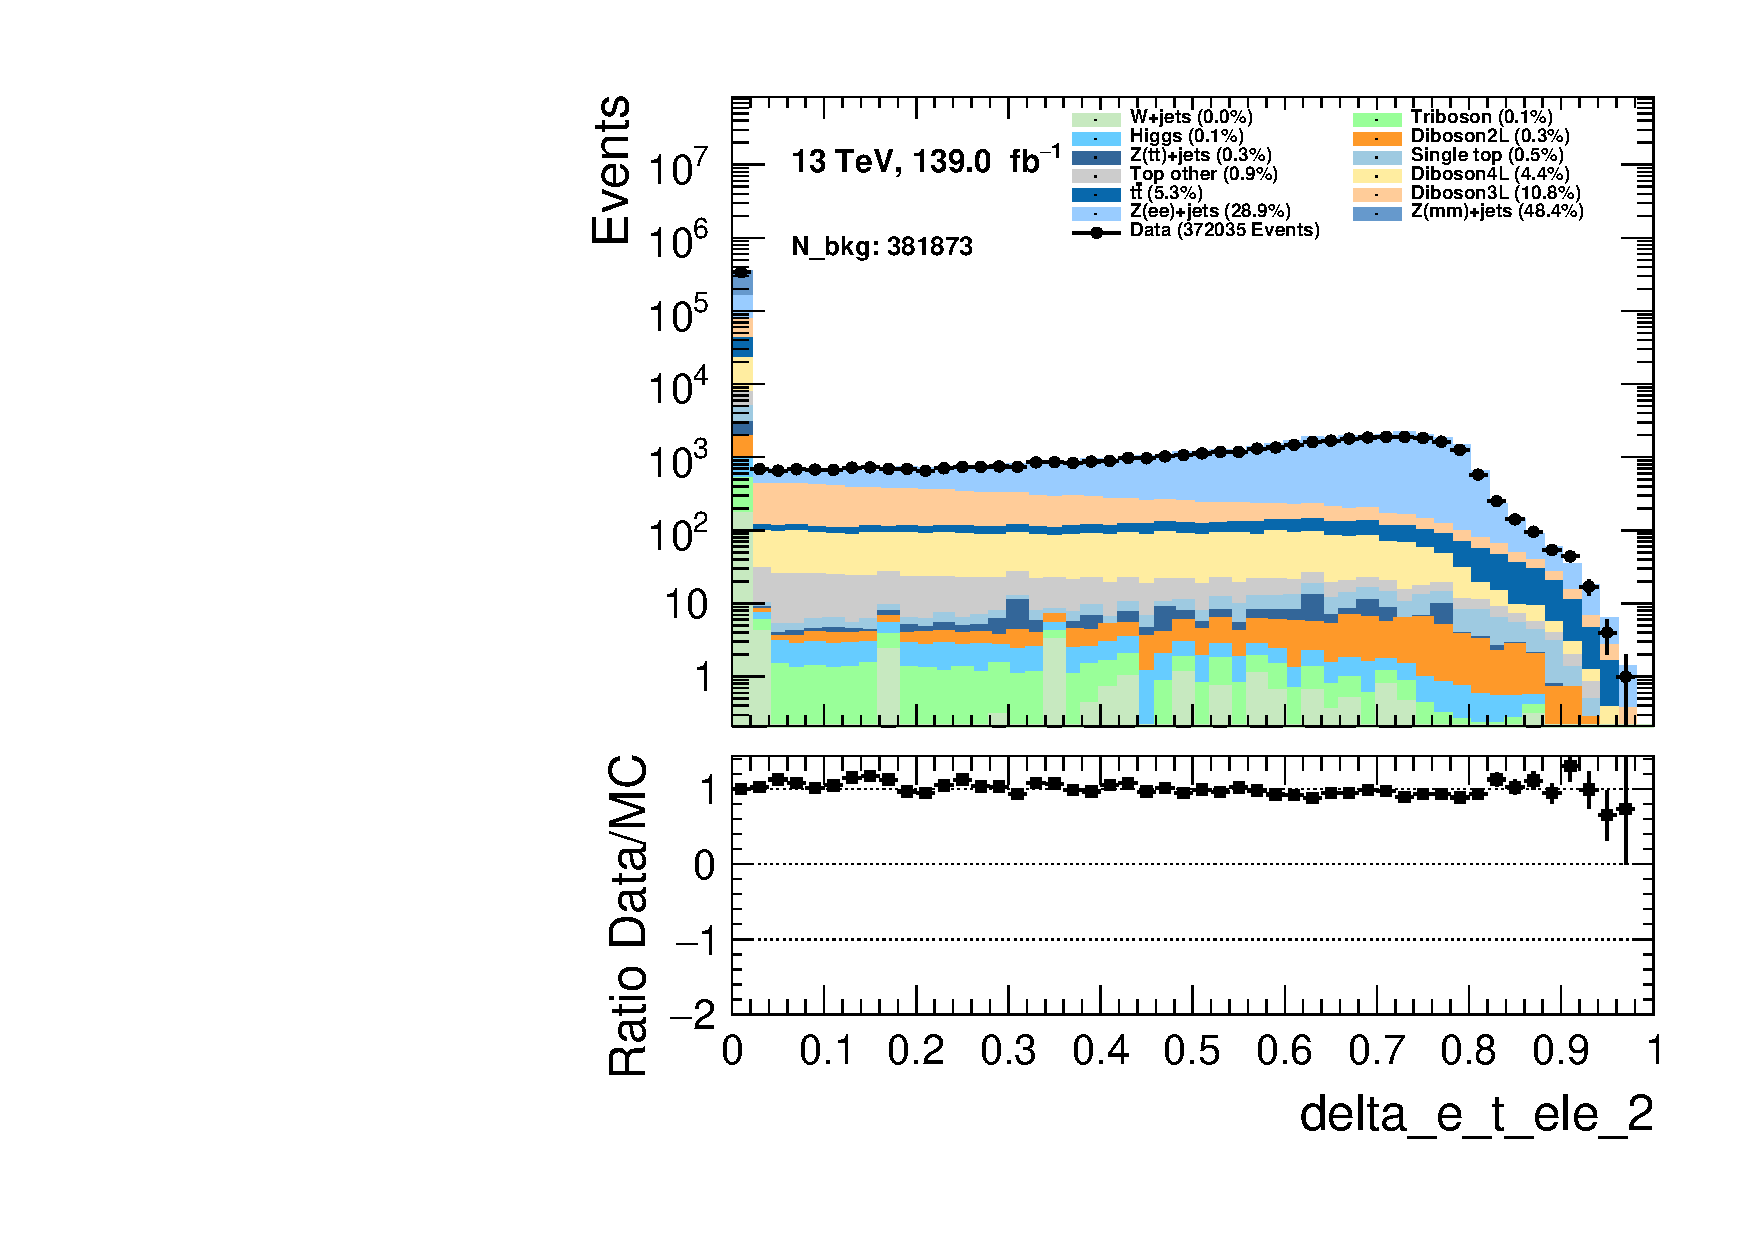
\includegraphics[width=\textwidth]{Figures/MC_Data_comp/delta_e_t_ele_2.pdf}
        \caption{Transverse energy imbalance for the third electron.}
        \label{fig:delta_e_t_ele_2}
    \end{subfigure}
    \hfill 
    \begin{subfigure}{.49\textwidth}
        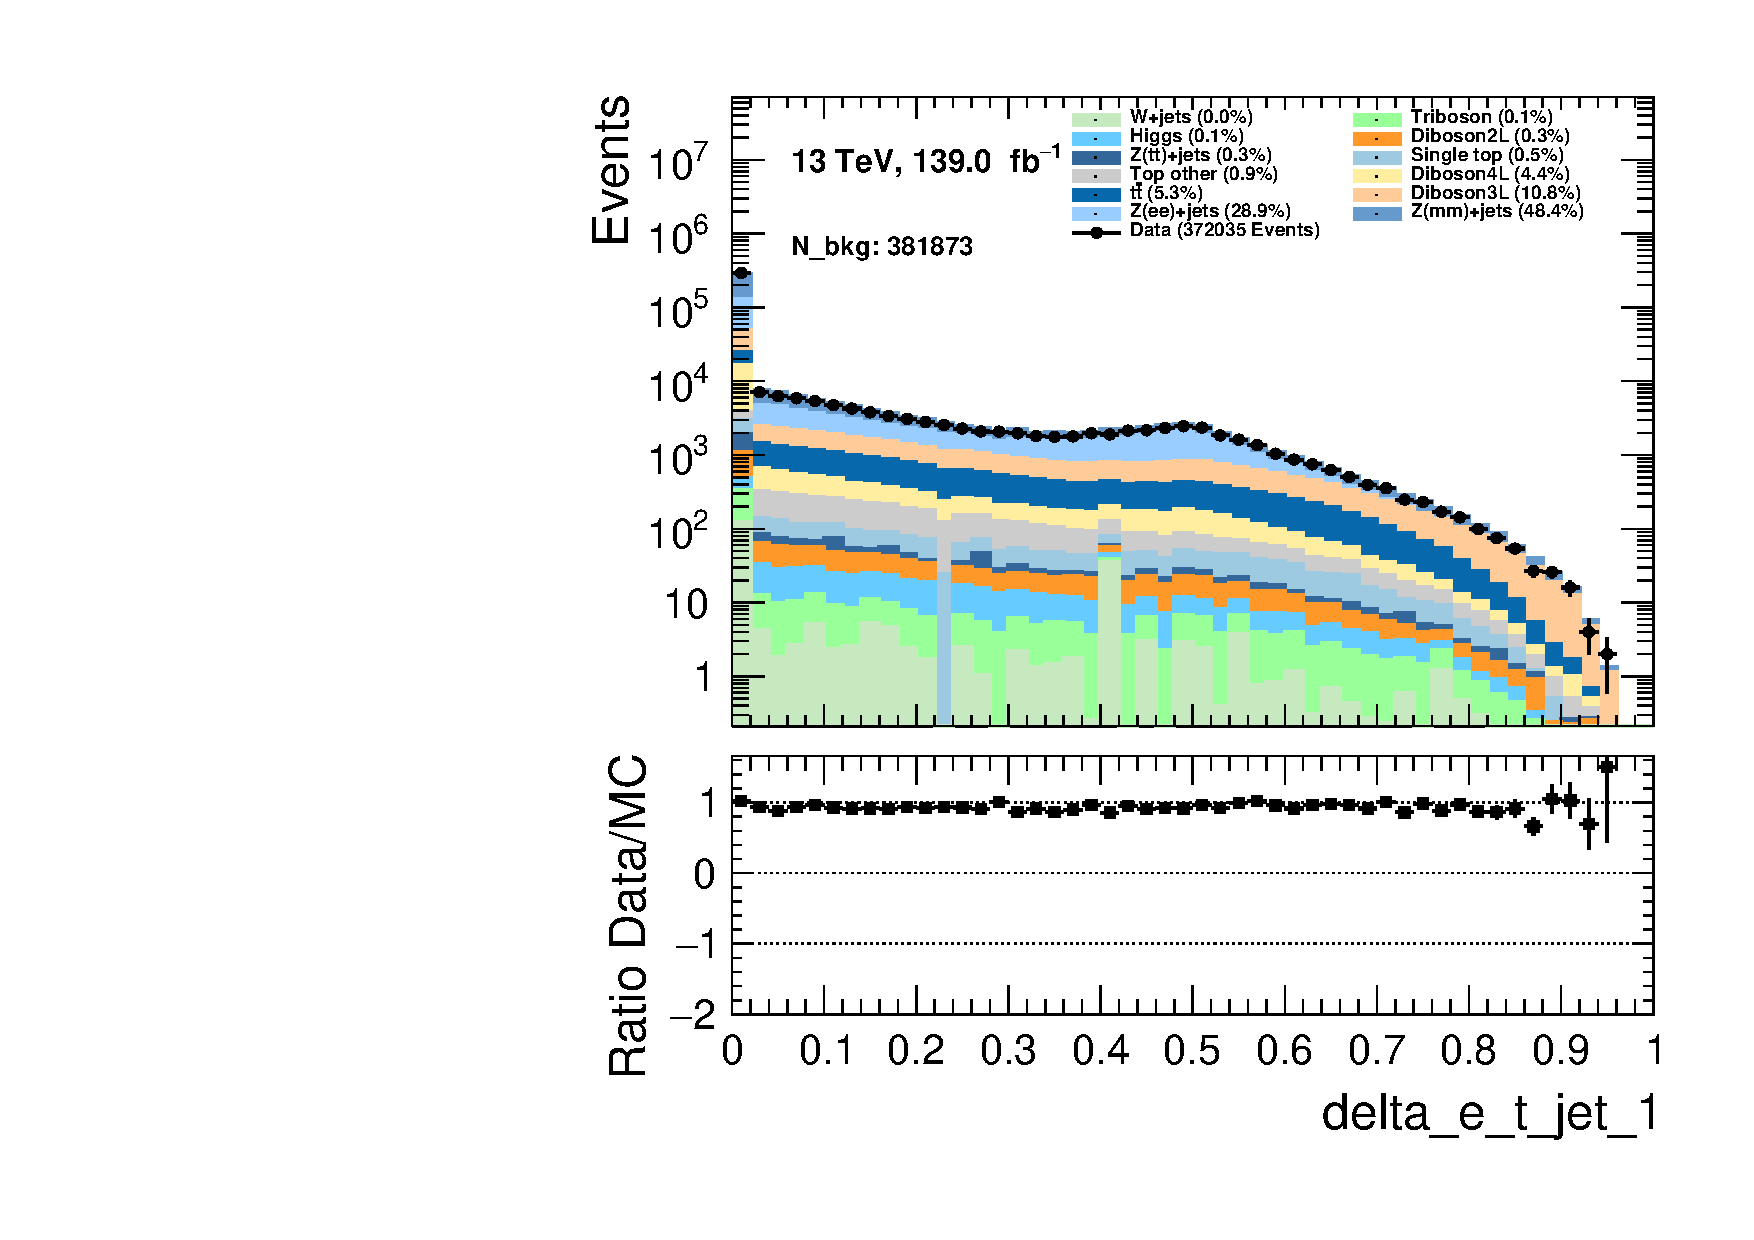
\includegraphics[width=\textwidth]{Figures/MC_Data_comp/delta_e_t_jet_1.pdf}
        \caption{ Transverse energy imbalance for the second jet.}
        \label{fig:delta_e_t_jet1}
    \end{subfigure}
    \hfill
    \begin{subfigure}{.49\textwidth}
        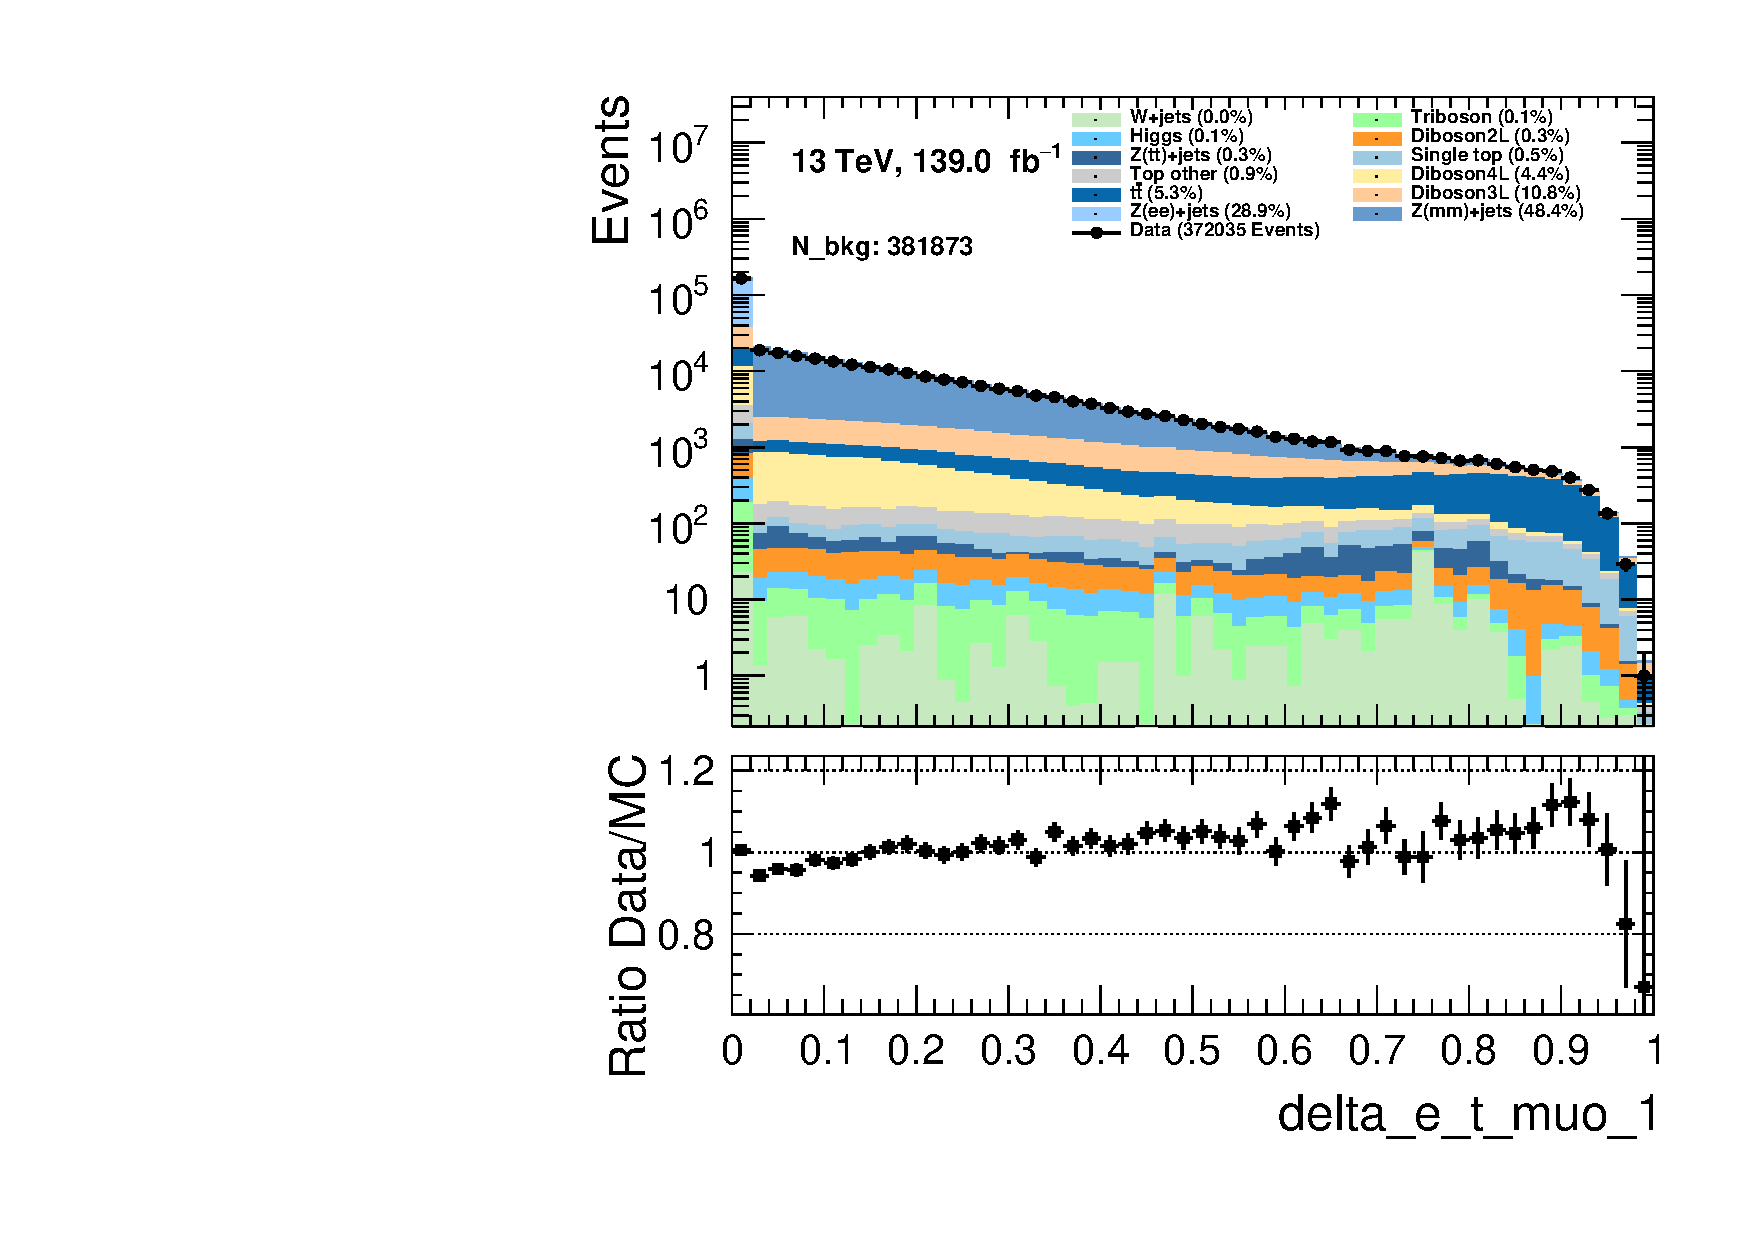
\includegraphics[width=\textwidth]{Figures/MC_Data_comp/delta_e_t_muo_1.pdf}
        \caption{Transverse energy imbalance for the second muon. }
        \label{fig:delta_e_t_muo1}
    \end{subfigure}
    \hfill       
    \caption{The four figures in this plot contains the transverse energy imbalance for the second muon and jet as well as the second and third electron. }
    \label{fig:batch1_feats}
\end{figure}

\begin{figure}
    \centering
    \begin{subfigure}{.49\textwidth}
        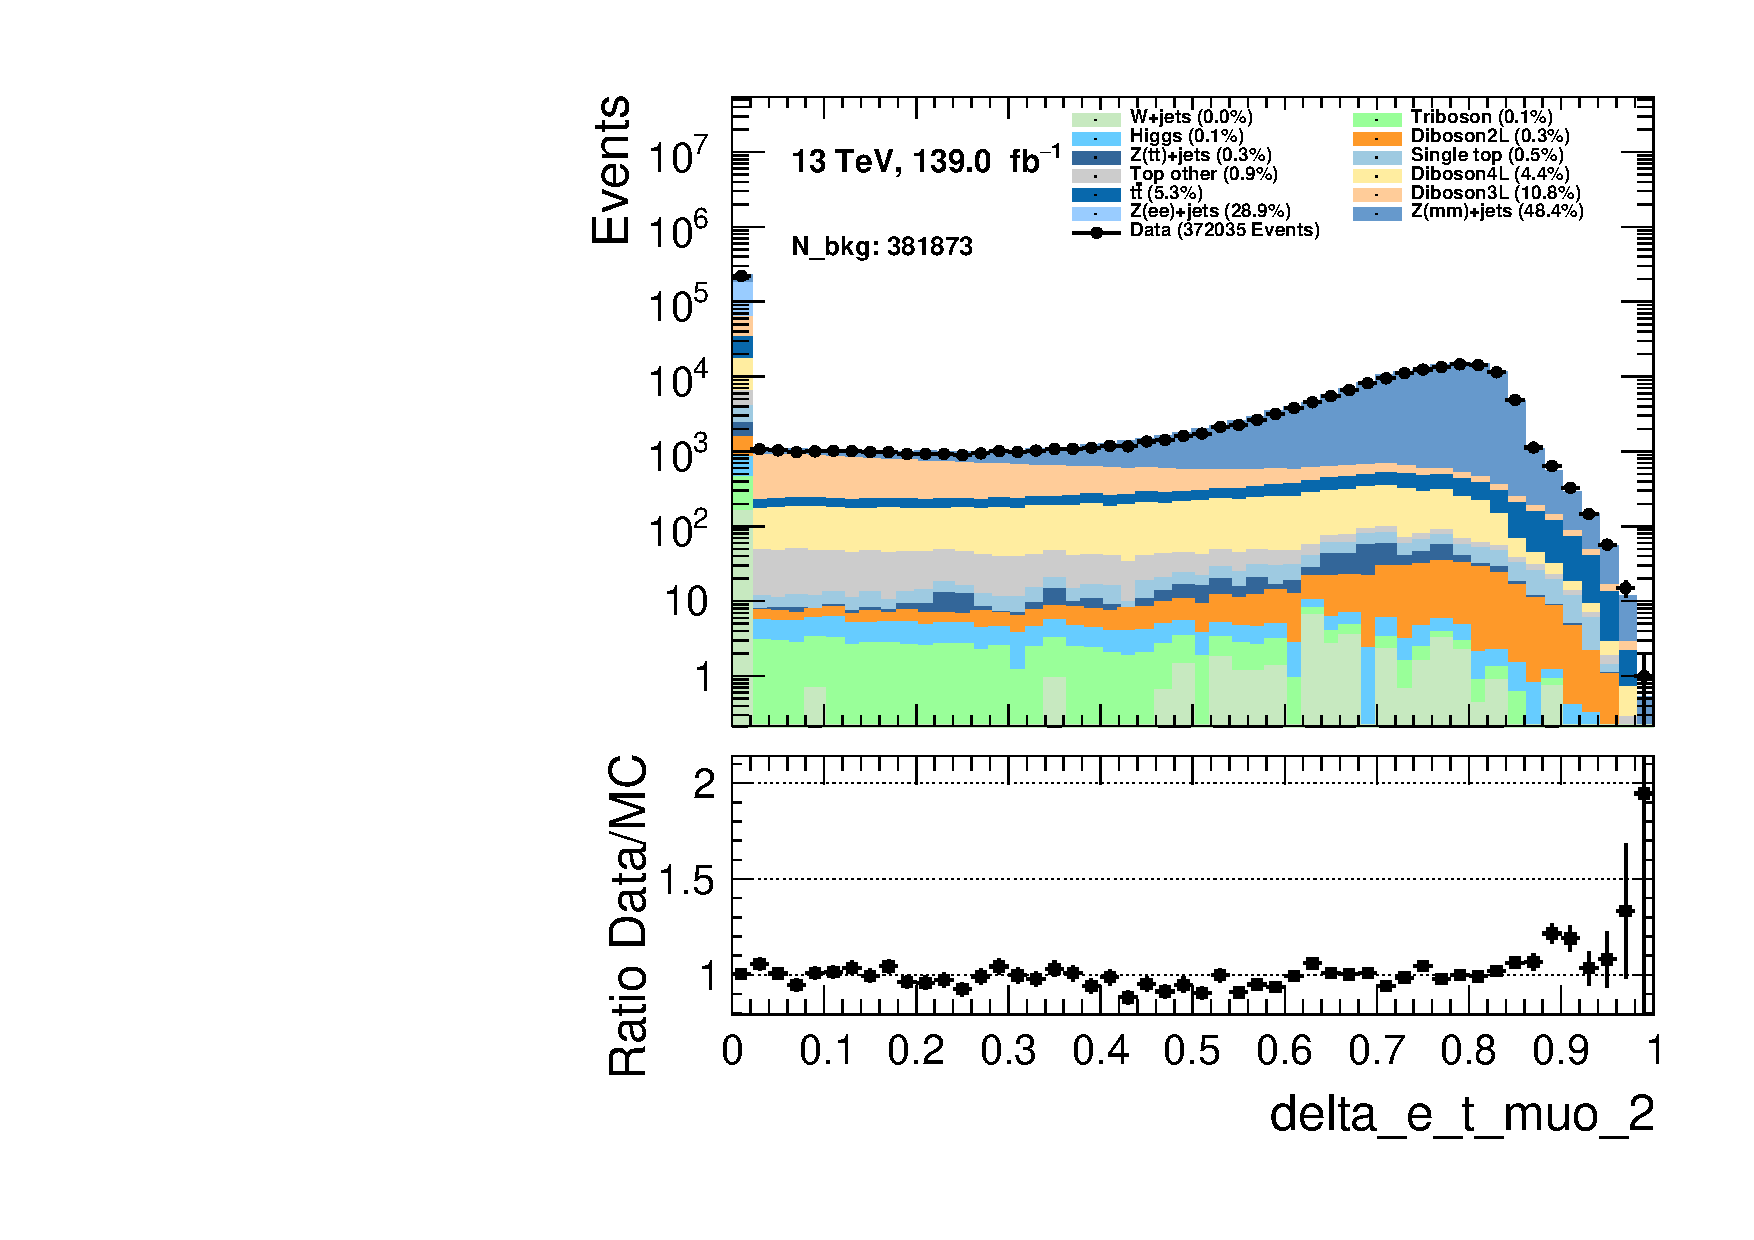
\includegraphics[width=\textwidth]{Figures/MC_Data_comp/delta_e_t_muo_2.pdf}
        \caption{Transverse energy imbalance for the third muon.}
        \label{fig:delta_e_t_muo2}
    \end{subfigure}
    \hfill
    \begin{subfigure}{.49\textwidth}
        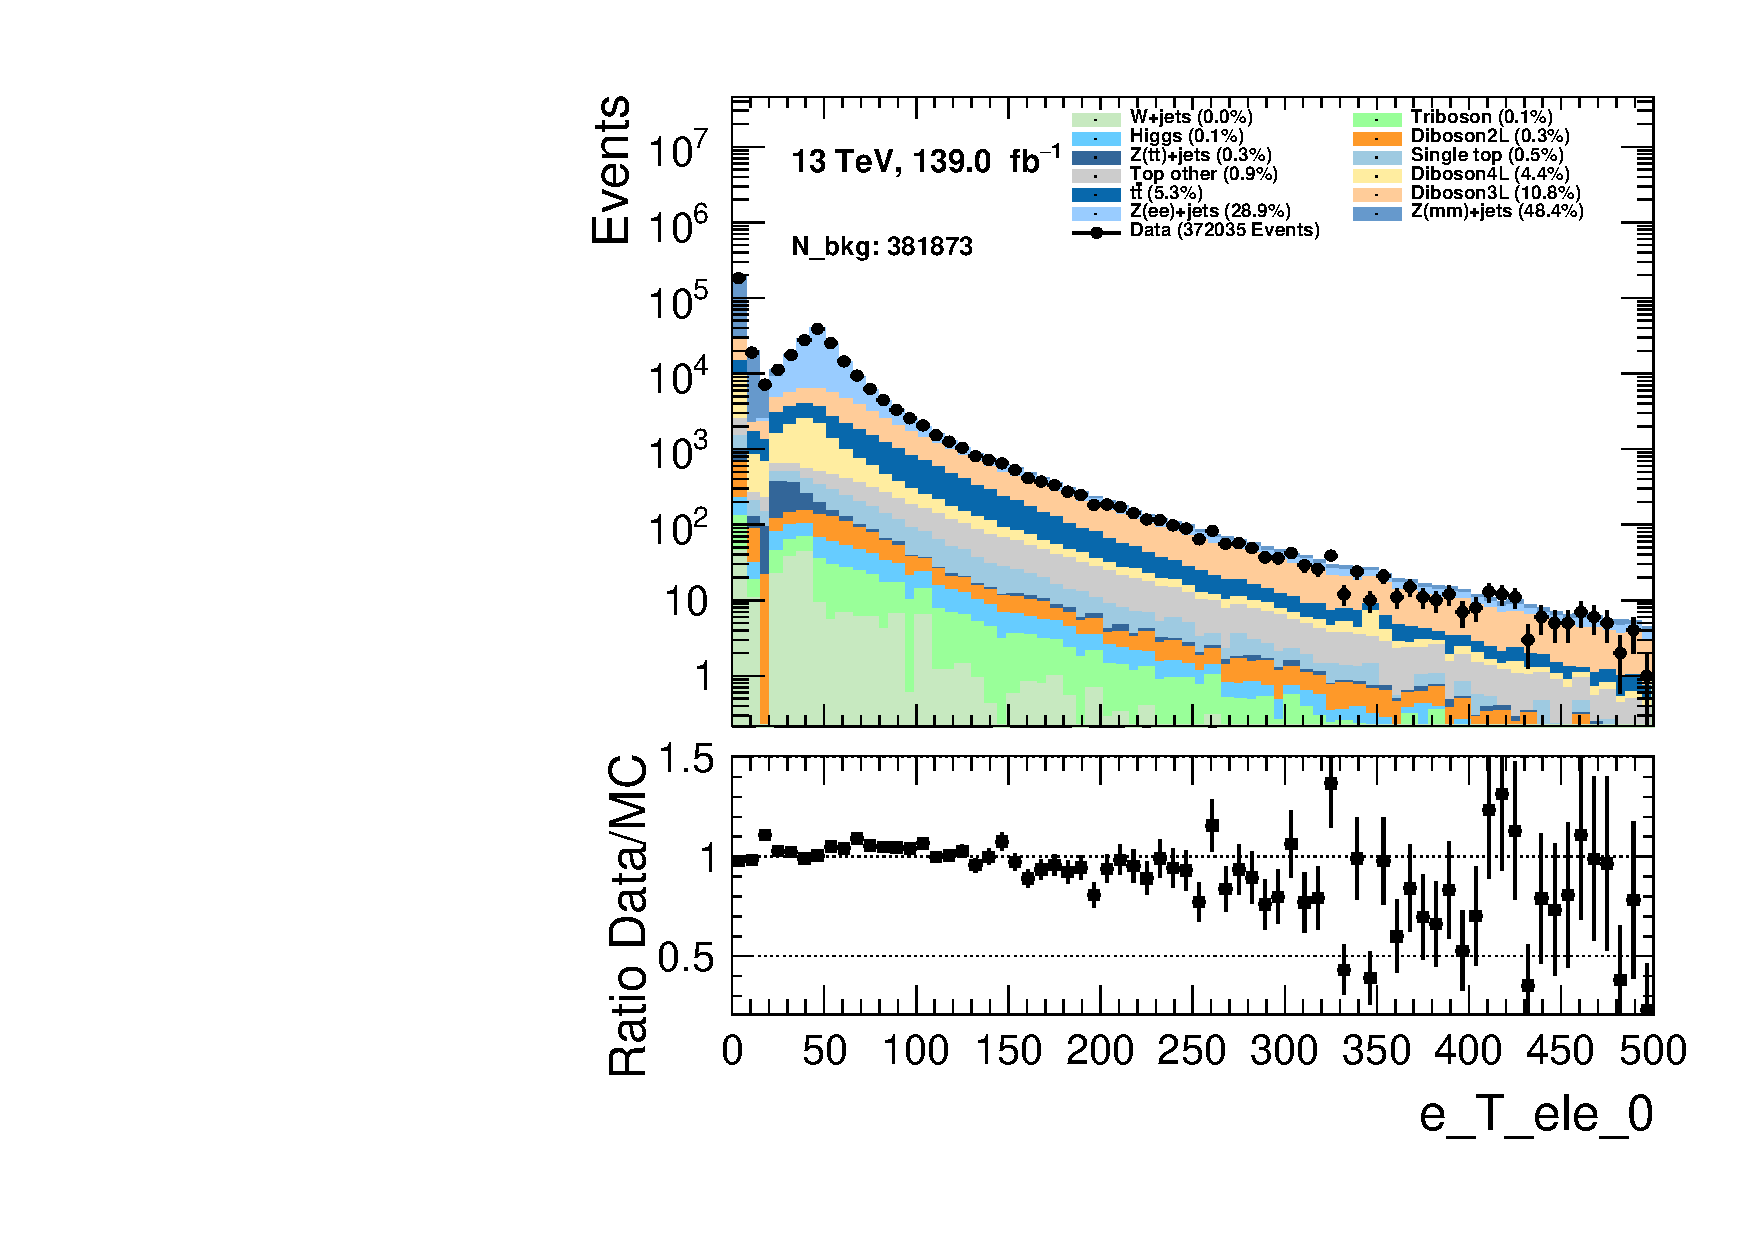
\includegraphics[width=\textwidth]{Figures/MC_Data_comp/e_T_ele_0.pdf}
        \caption{ Transverse energy for the first electron.}
        \label{fig:e_T_ele0}
    \end{subfigure}
    \hfill 
    \begin{subfigure}{.49\textwidth}
        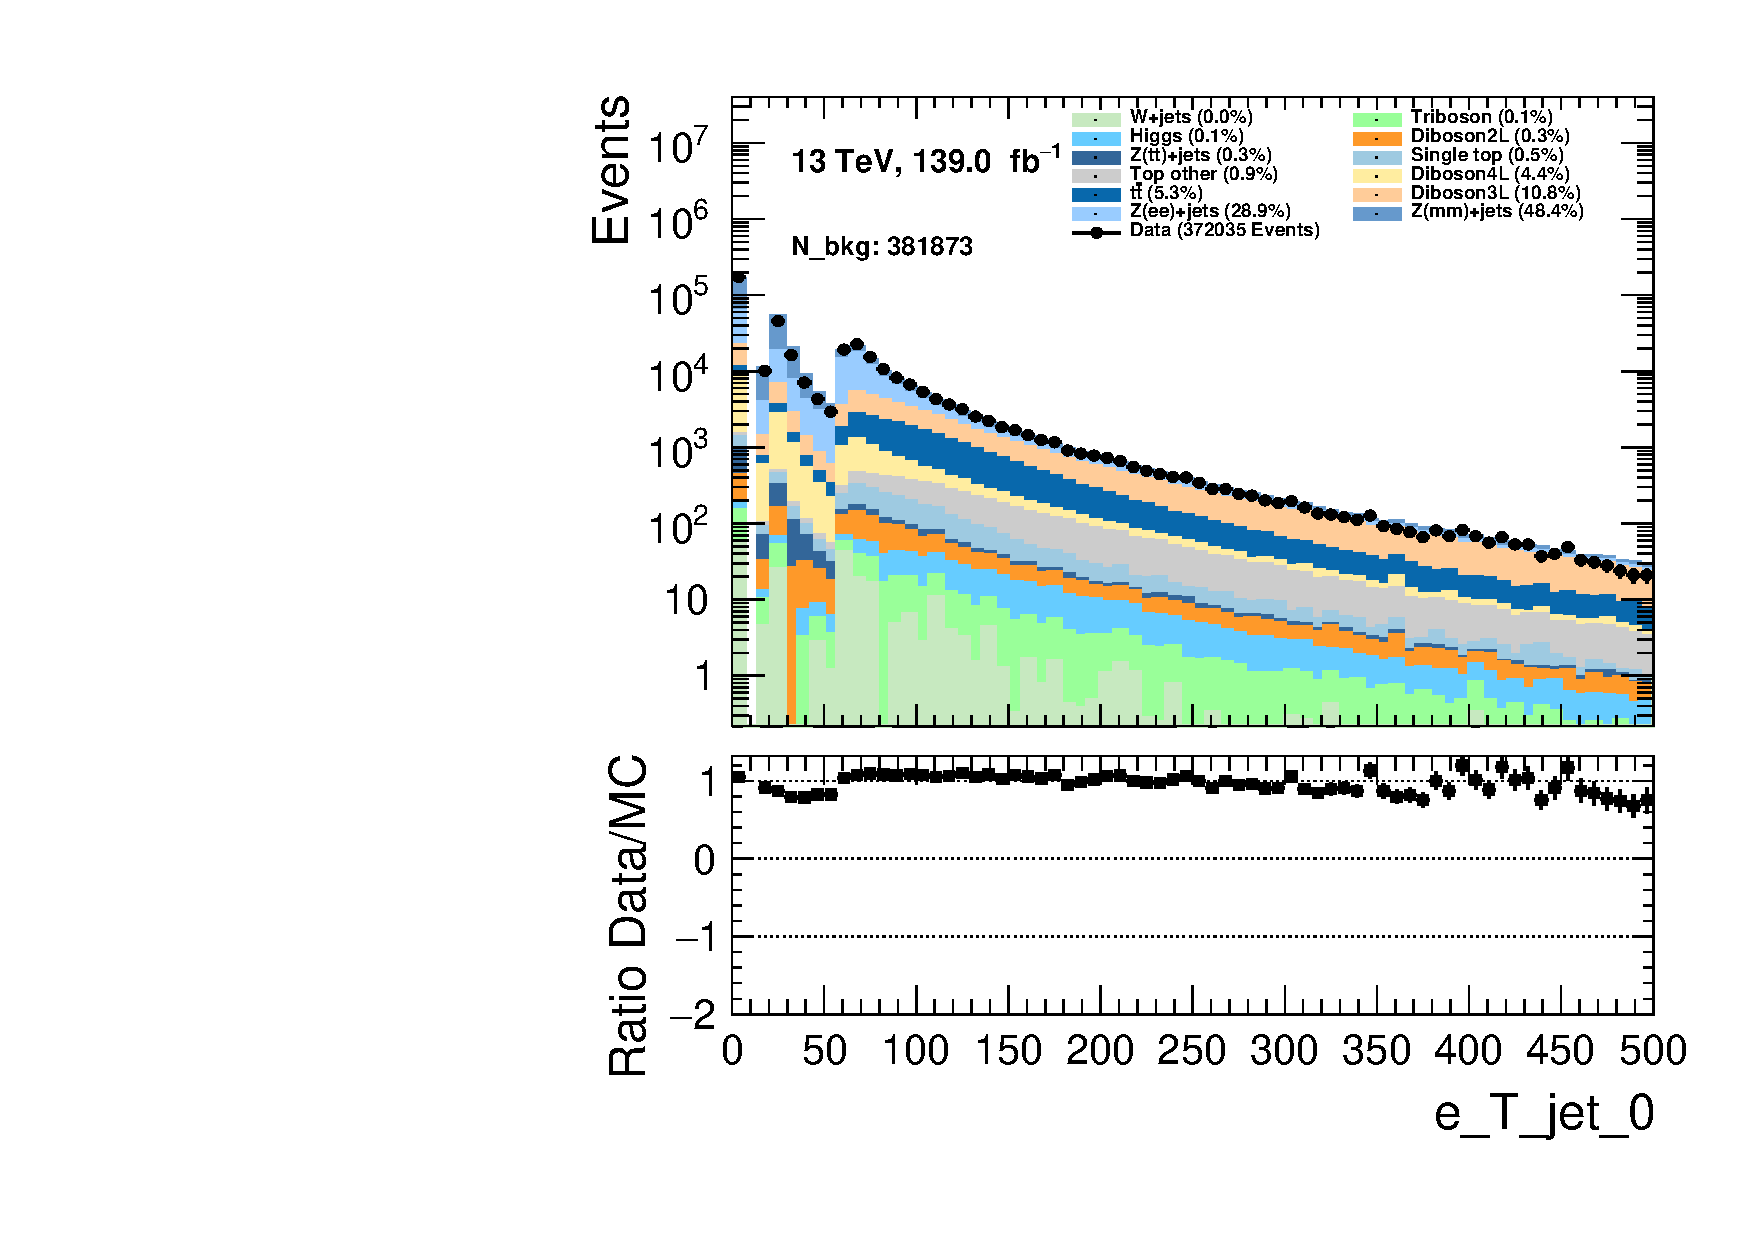
\includegraphics[width=\textwidth]{Figures/MC_Data_comp/e_T_jet_0.pdf}
        \caption{Transverse energy for the first jet. }
        \label{fig:e_T_jet0}
    \end{subfigure}
    \hfill
    \begin{subfigure}{.49\textwidth}
        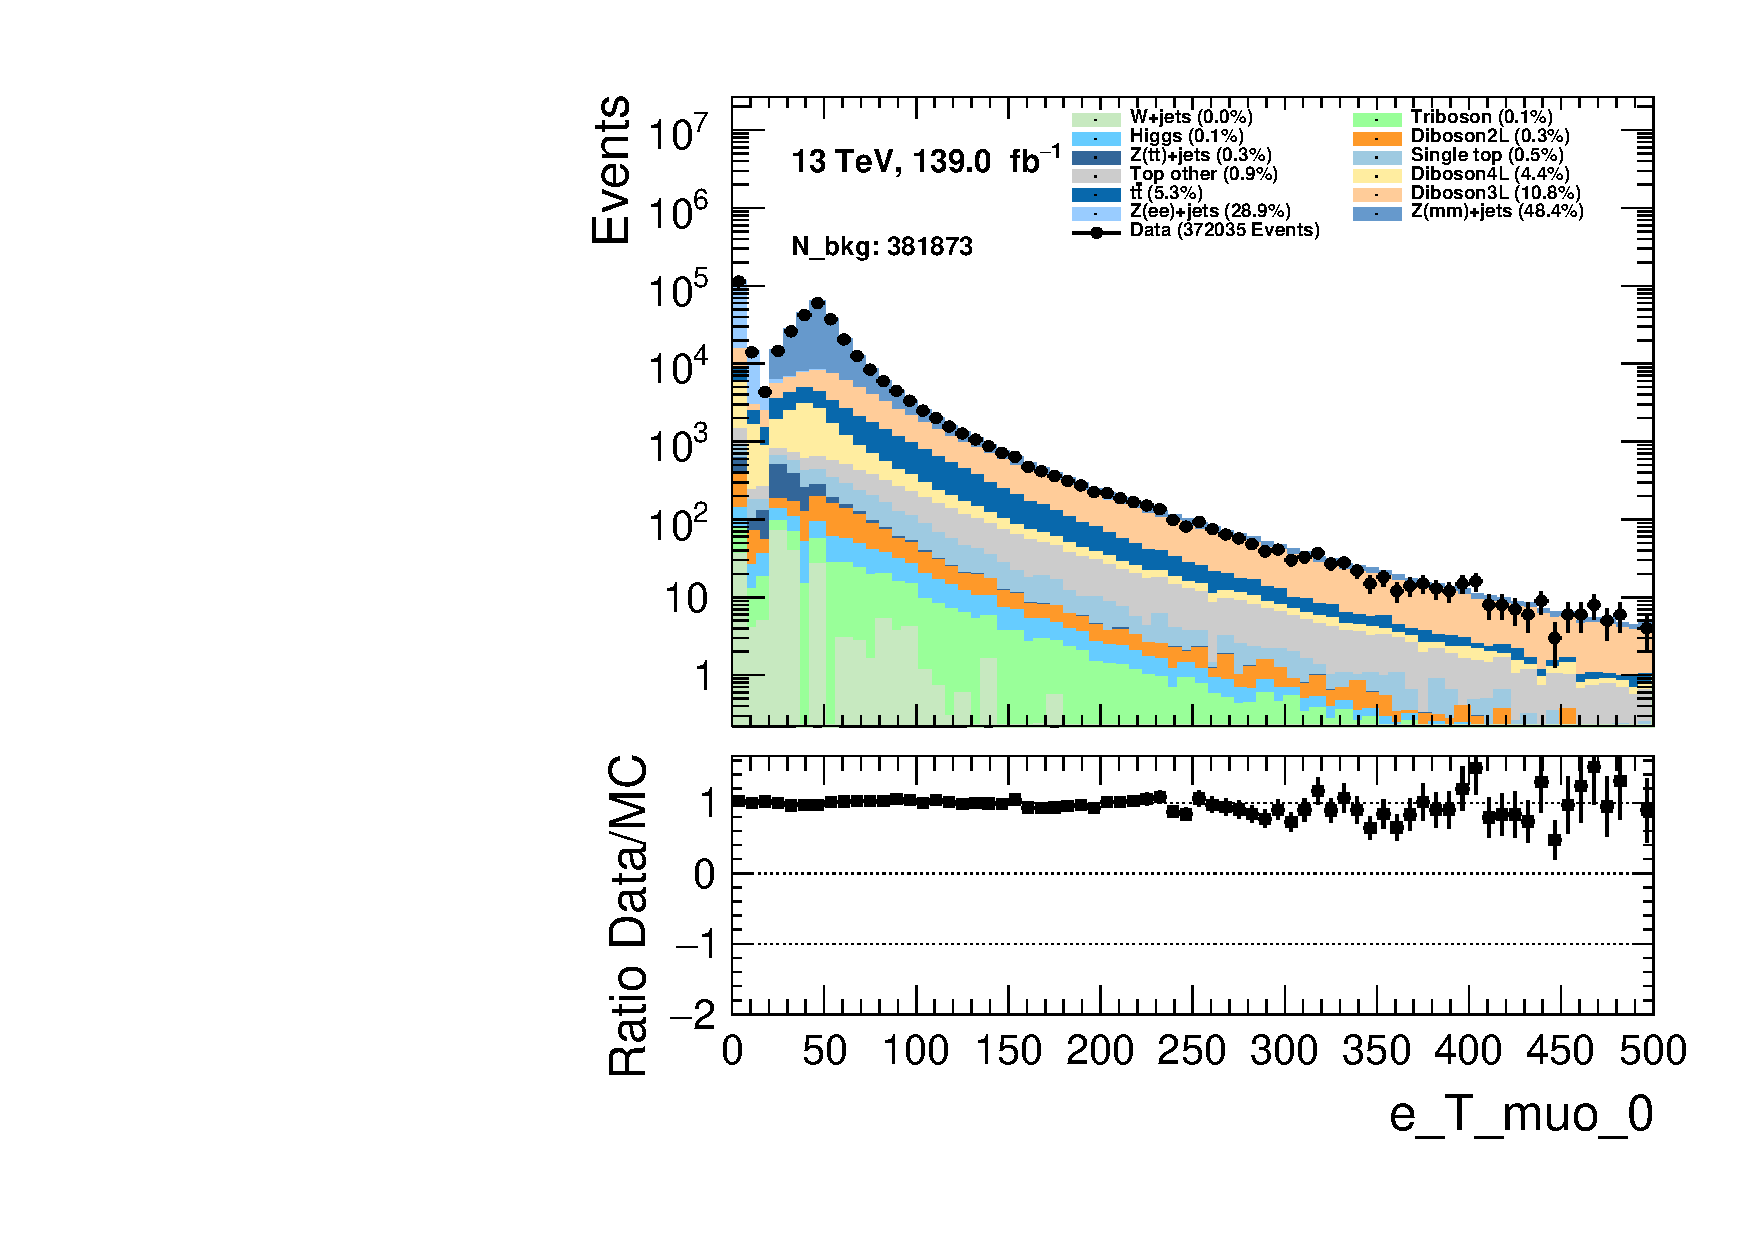
\includegraphics[width=\textwidth]{Figures/MC_Data_comp/e_T_muo_0.pdf}
        \caption{Transverse energy for the first moun. }
        \label{fig:e_T_muo0}
    \end{subfigure}
    \hfill       
    \caption{Transverse energy for the first jet, electron and muon, as well as the transverse energy imbalance for the third muon. }
    \label{fig:batch2_feats}
\end{figure}

\begin{figure}
    \centering
    \begin{subfigure}{.49\textwidth}
        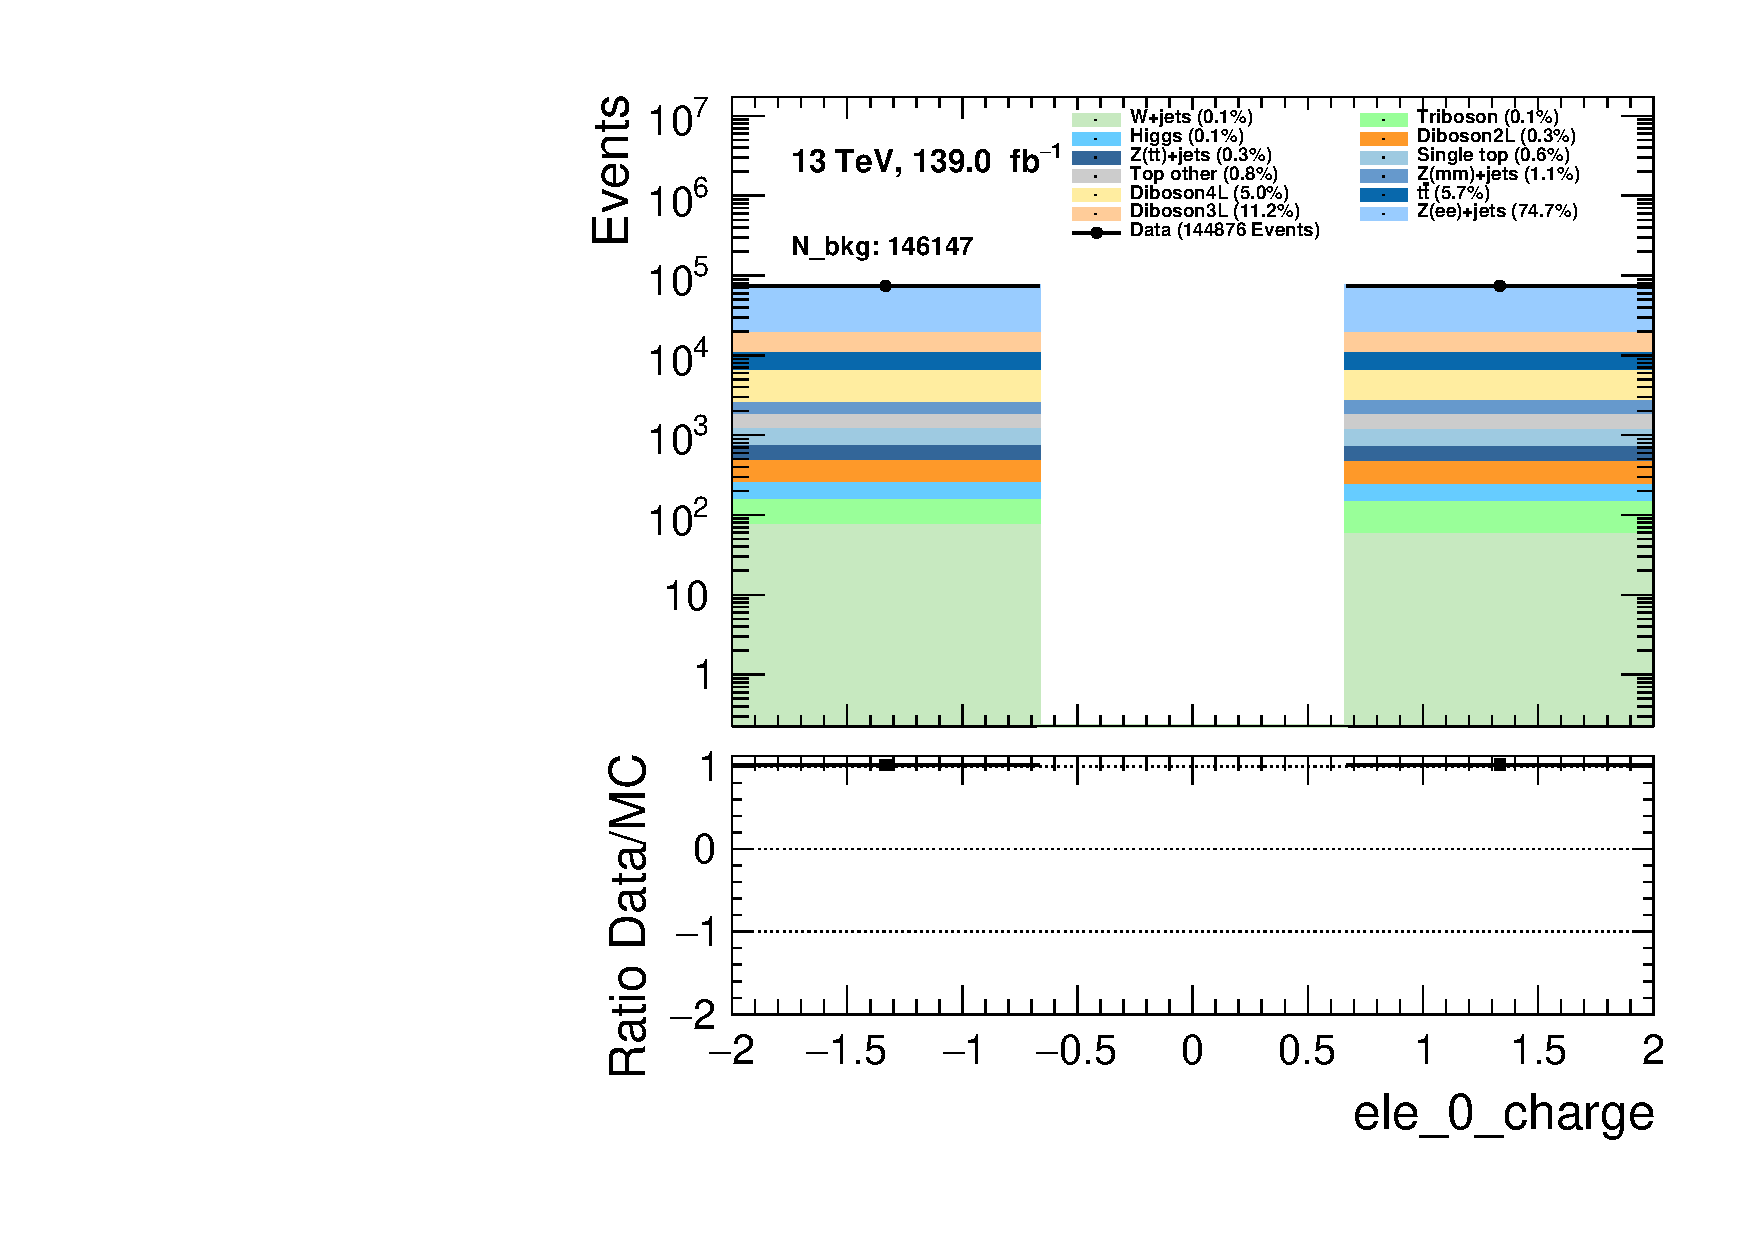
\includegraphics[width=\textwidth]{Figures/MC_Data_comp/ele_0_charge.pdf}
        \caption{Change distribution for the first electron.}
        \label{fig:ele_0_charge}
    \end{subfigure}
    \hfill
    \begin{subfigure}{.49\textwidth}
        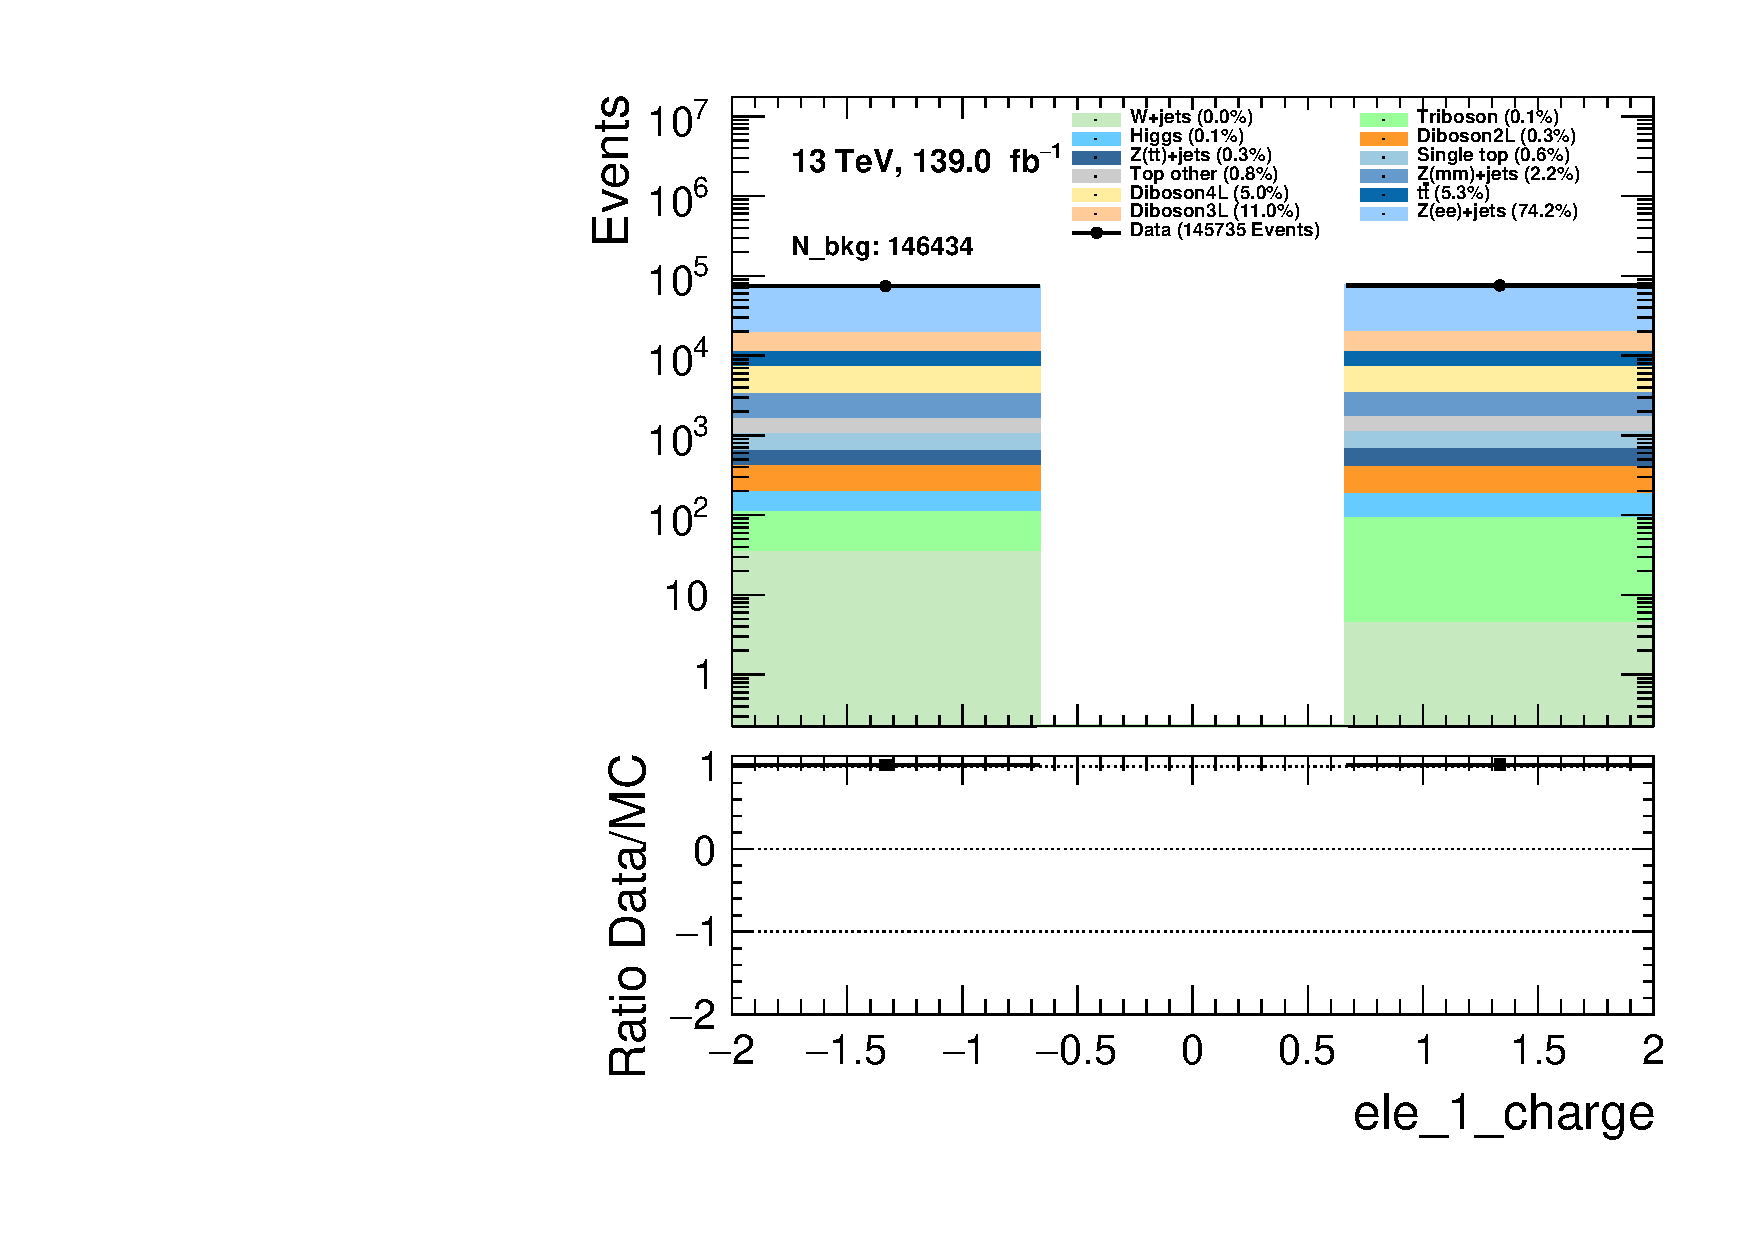
\includegraphics[width=\textwidth]{Figures/MC_Data_comp/ele_1_charge.pdf}
        \caption{Change distribution for the second electron. }
        \label{fig:ele_1_charge}
    \end{subfigure}
    \hfill 
    \begin{subfigure}{.49\textwidth}
        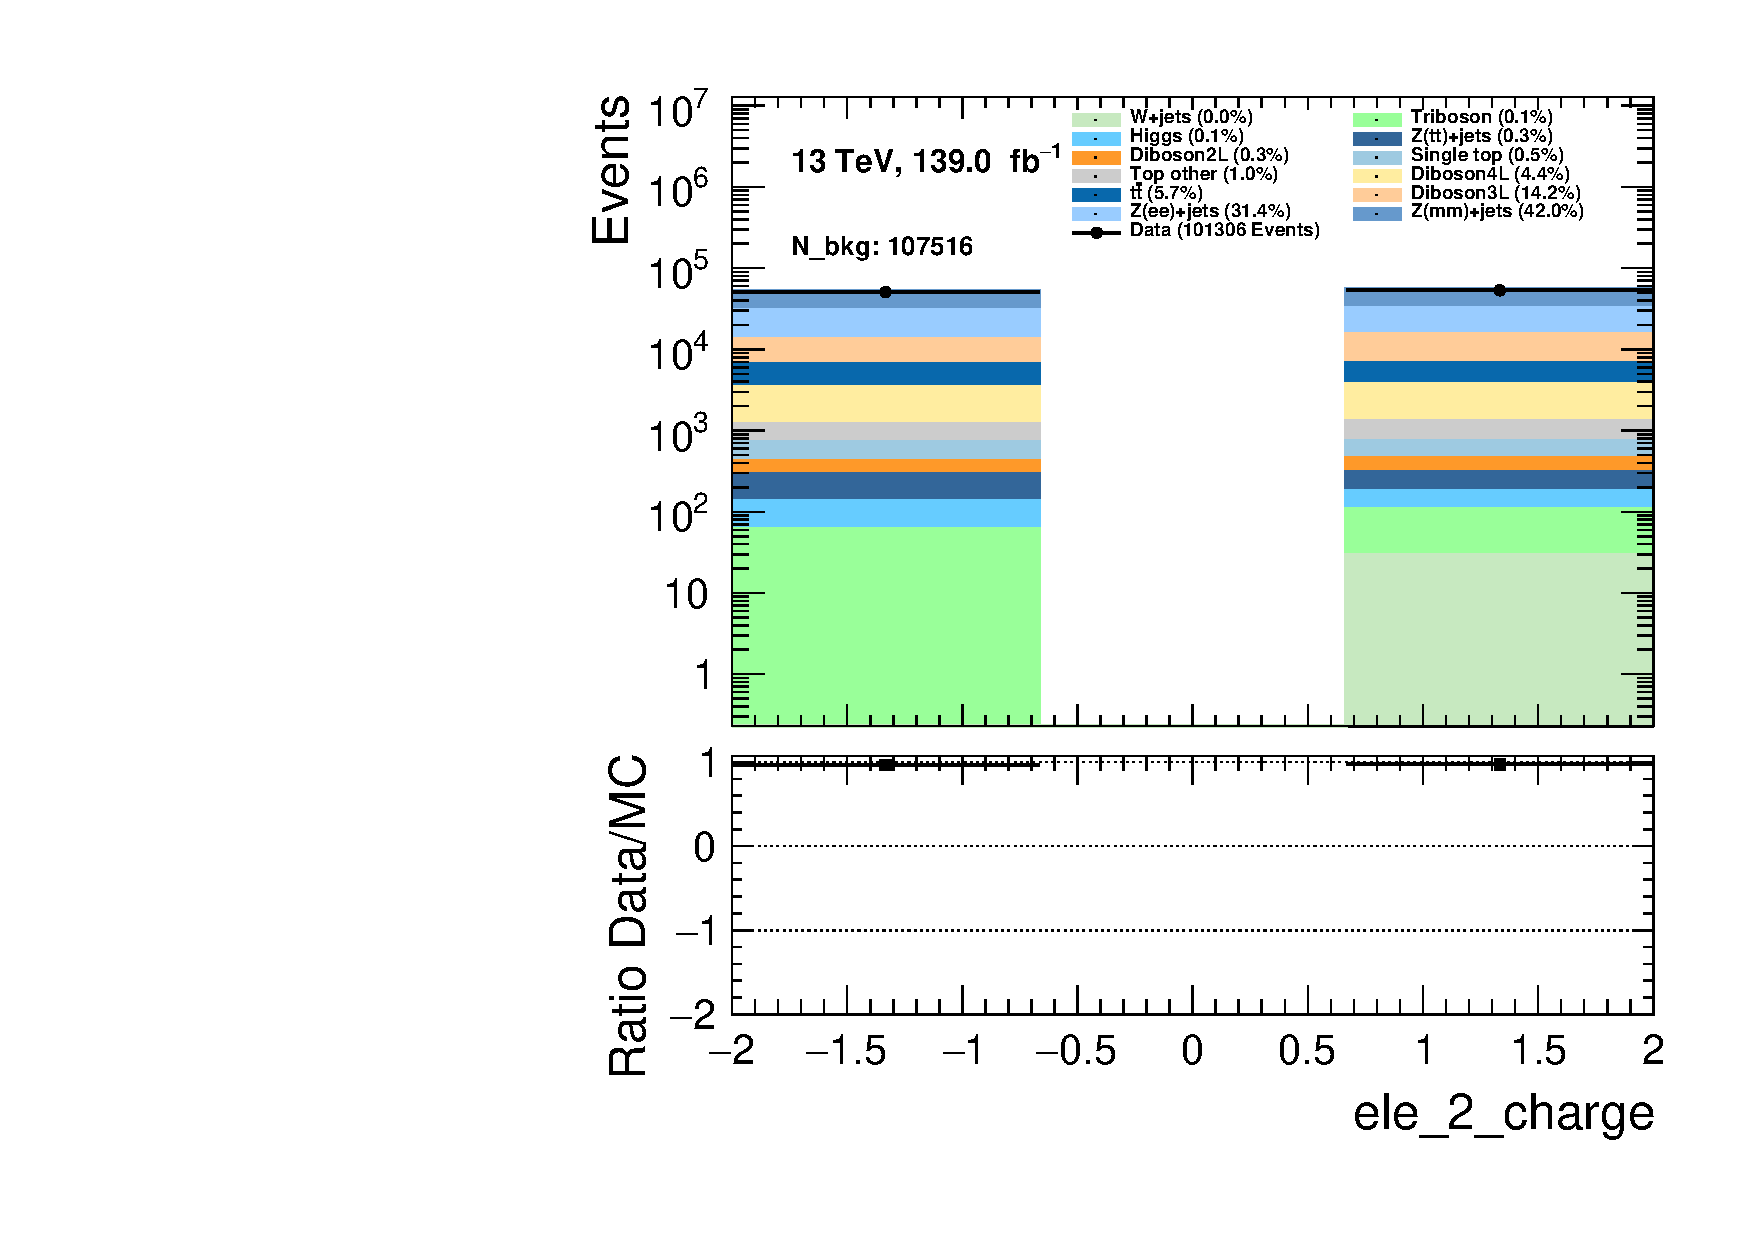
\includegraphics[width=\textwidth]{Figures/MC_Data_comp/ele_2_charge.pdf}
        \caption{Change distribution for the third electron. }
        \label{fig:ele_2_charge}
    \end{subfigure}
    \hfill
    \begin{subfigure}{.49\textwidth}
        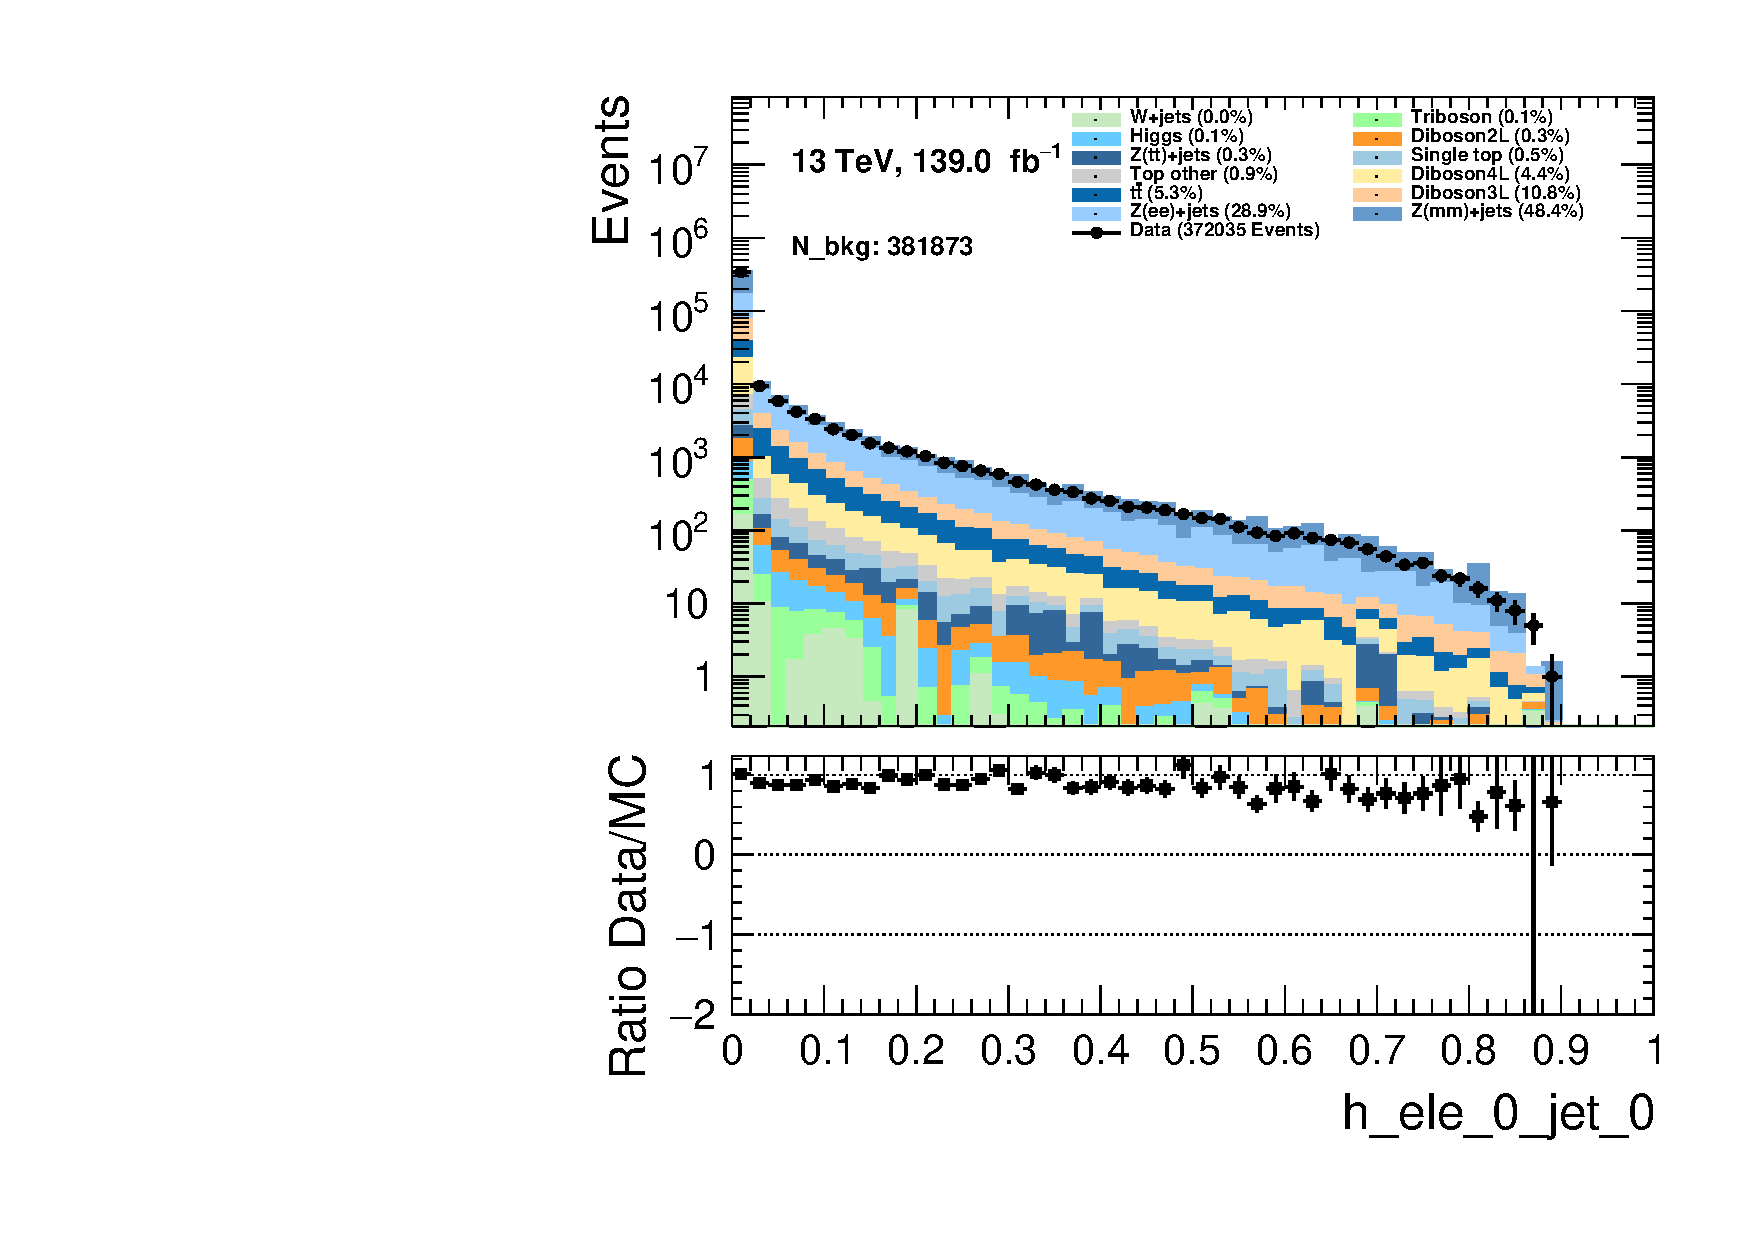
\includegraphics[width=\textwidth]{Figures/MC_Data_comp/h_ele_0_jet_0.pdf}
        \caption{ Longitudal component basd on rapidity difference between the first electron and first jet.}
        \label{fig:h_ele_0_jet_0}
    \end{subfigure}
    \hfill       
    \caption{Charge distribution for the three electrons, and longitudal component between first electron and first jet. }
    \label{fig:batch3_feats}
\end{figure}

\begin{figure}
    \centering
    \begin{subfigure}{.49\textwidth}
        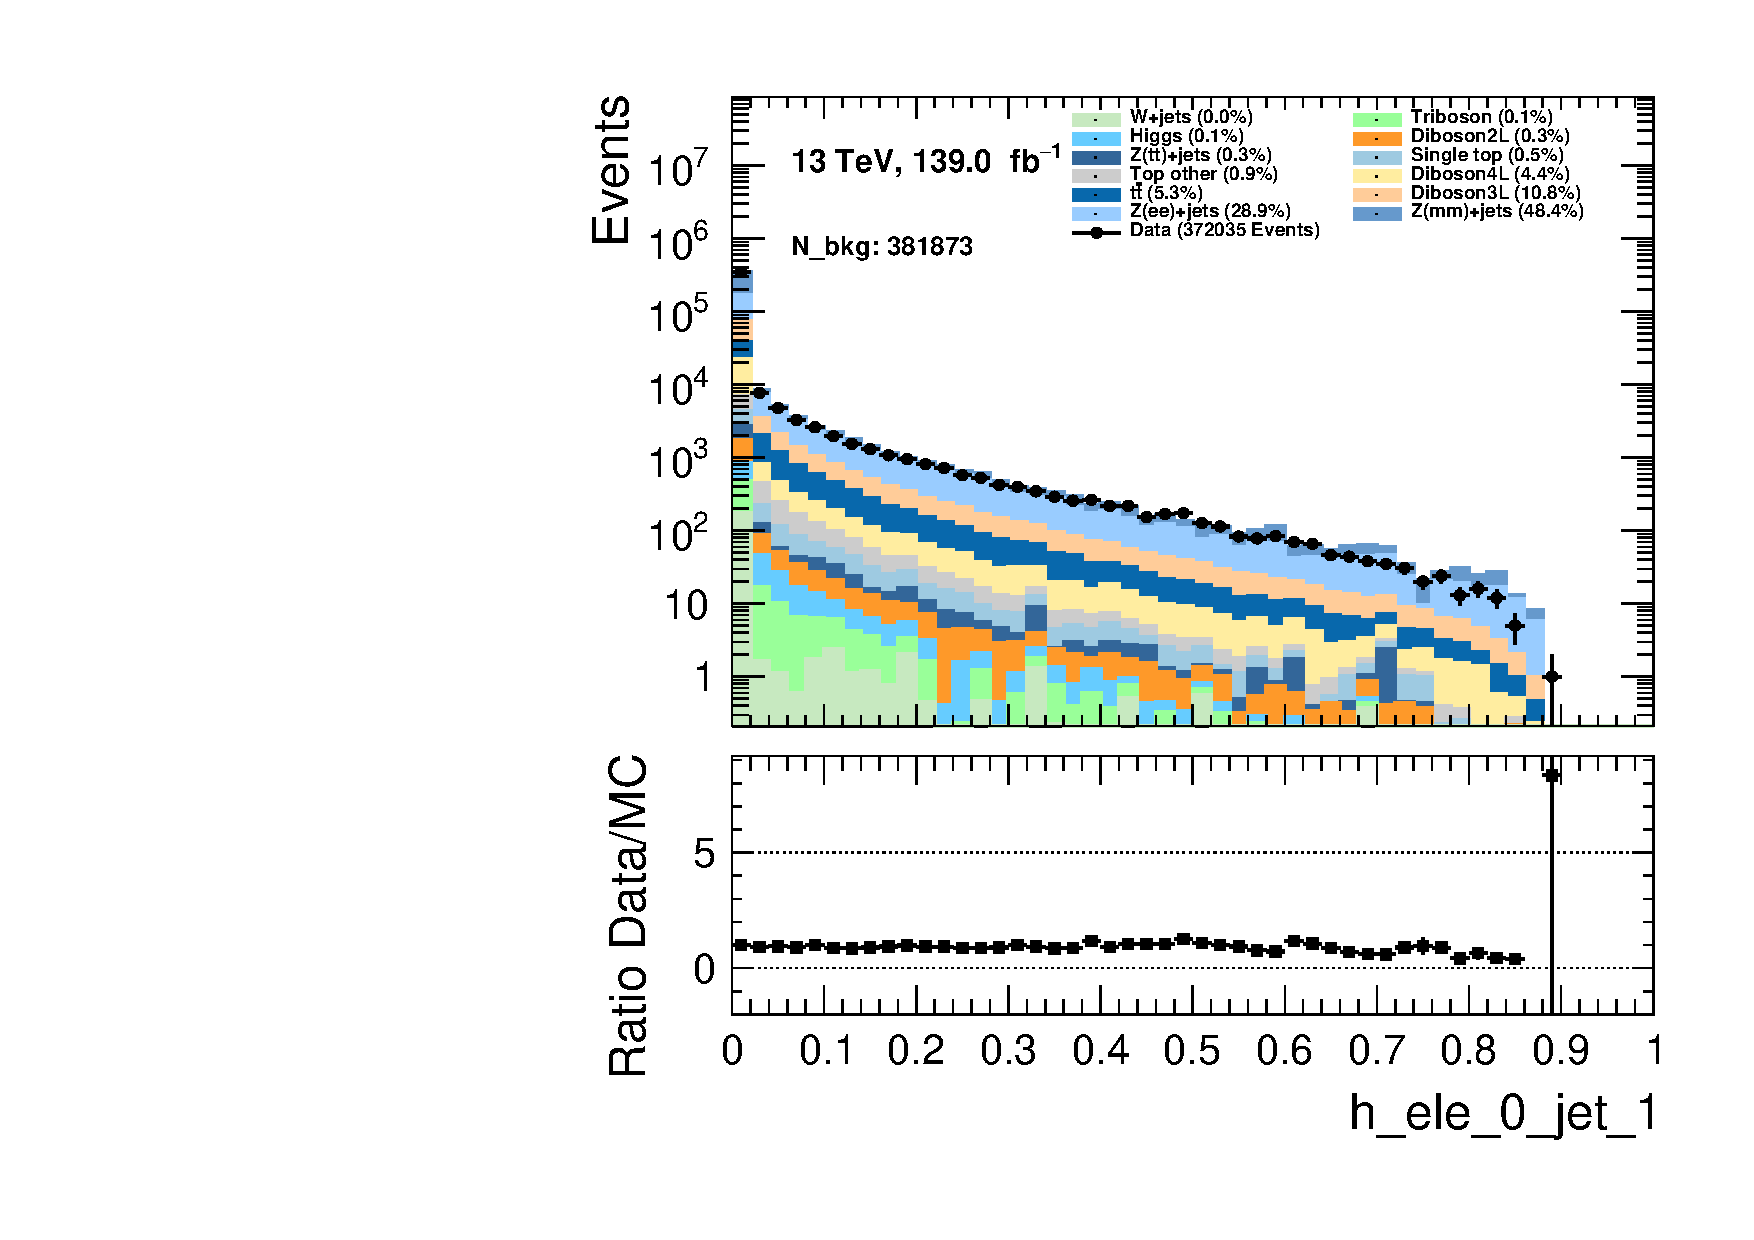
\includegraphics[width=\textwidth]{Figures/MC_Data_comp/h_ele_0_jet_1.pdf}
        \caption{Longitudal component between first electron and second jet.}
        \label{fig:h_ele_0_jet_1}
    \end{subfigure}
    \hfill
    \begin{subfigure}{.49\textwidth}
        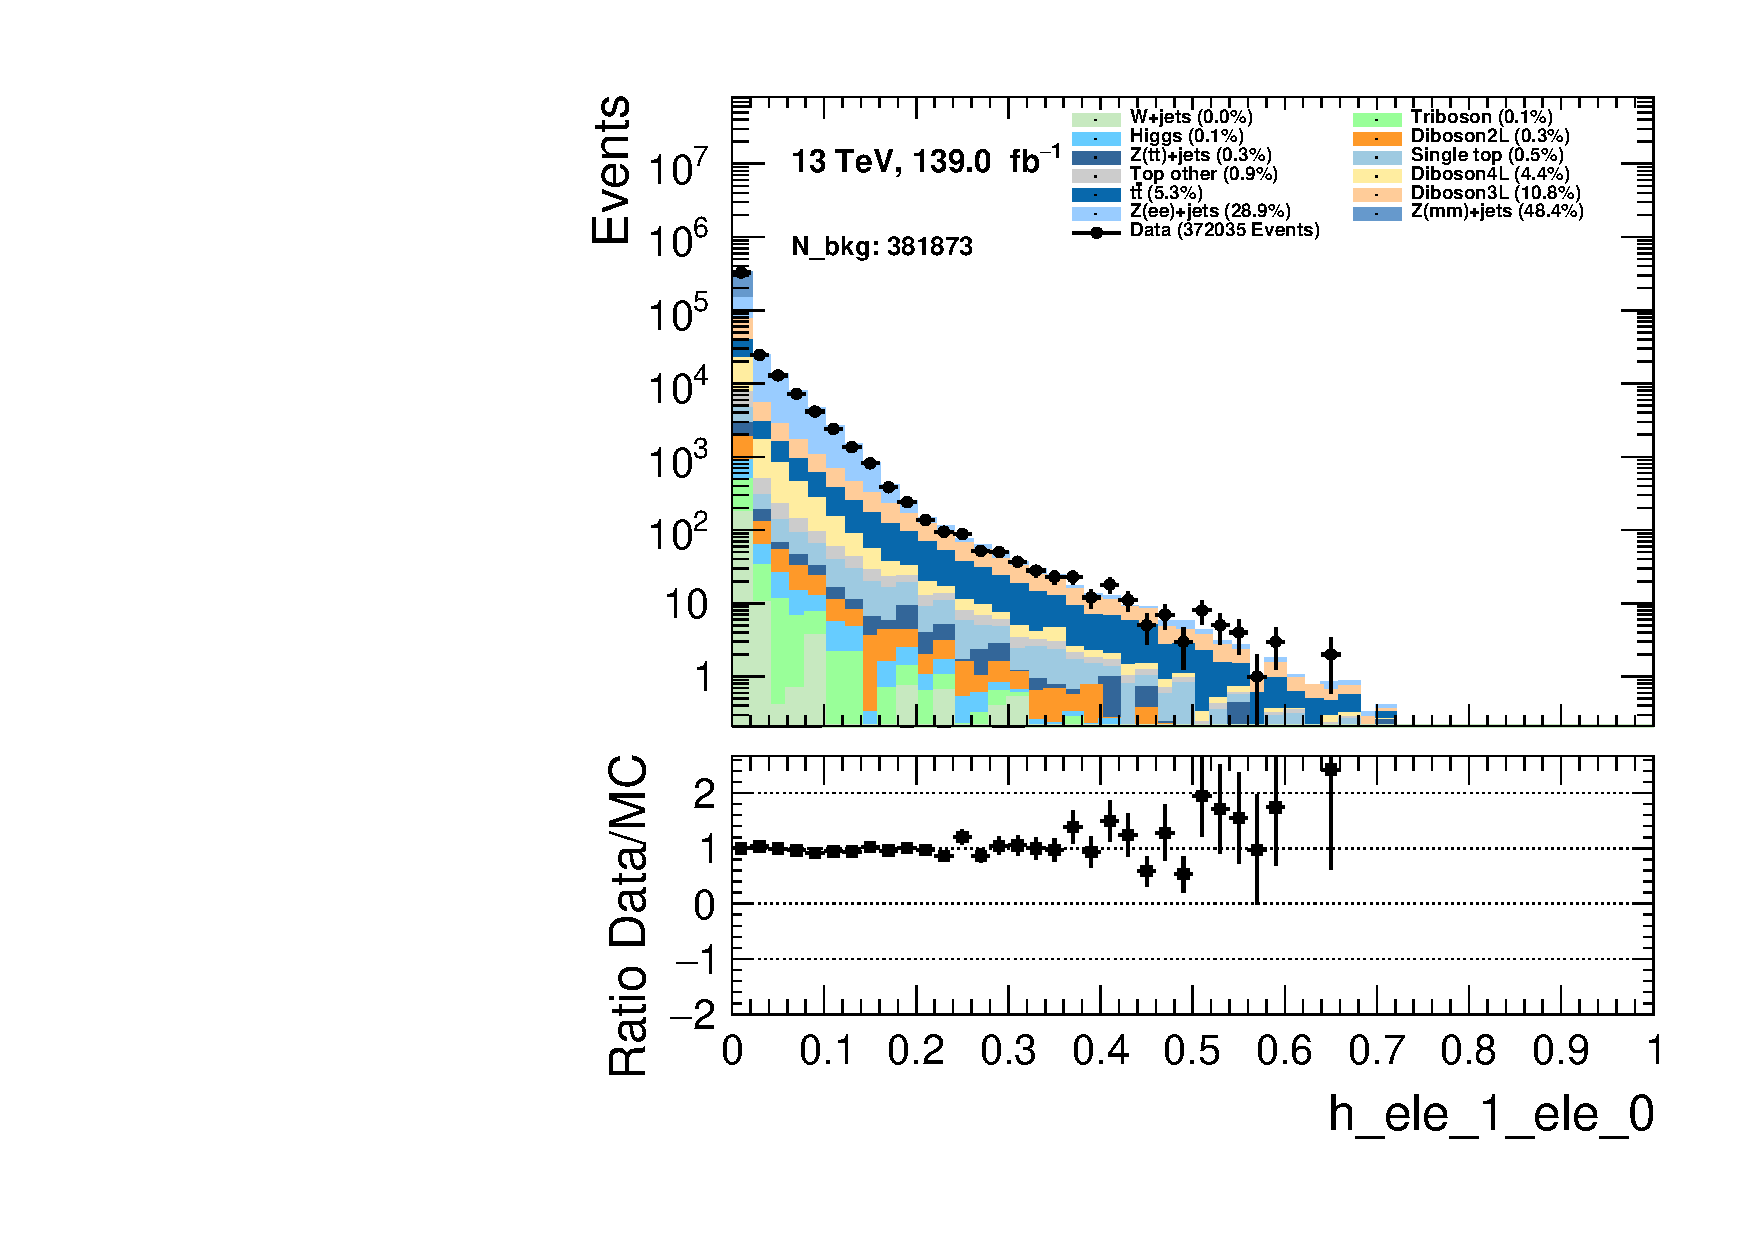
\includegraphics[width=\textwidth]{Figures/MC_Data_comp/h_ele_1_ele_0.pdf}
        \caption{Longitudal component between first and second electron.}
        \label{fig:h_ele_1_ele_0}
    \end{subfigure}
    \hfill 
    \begin{subfigure}{.49\textwidth}
        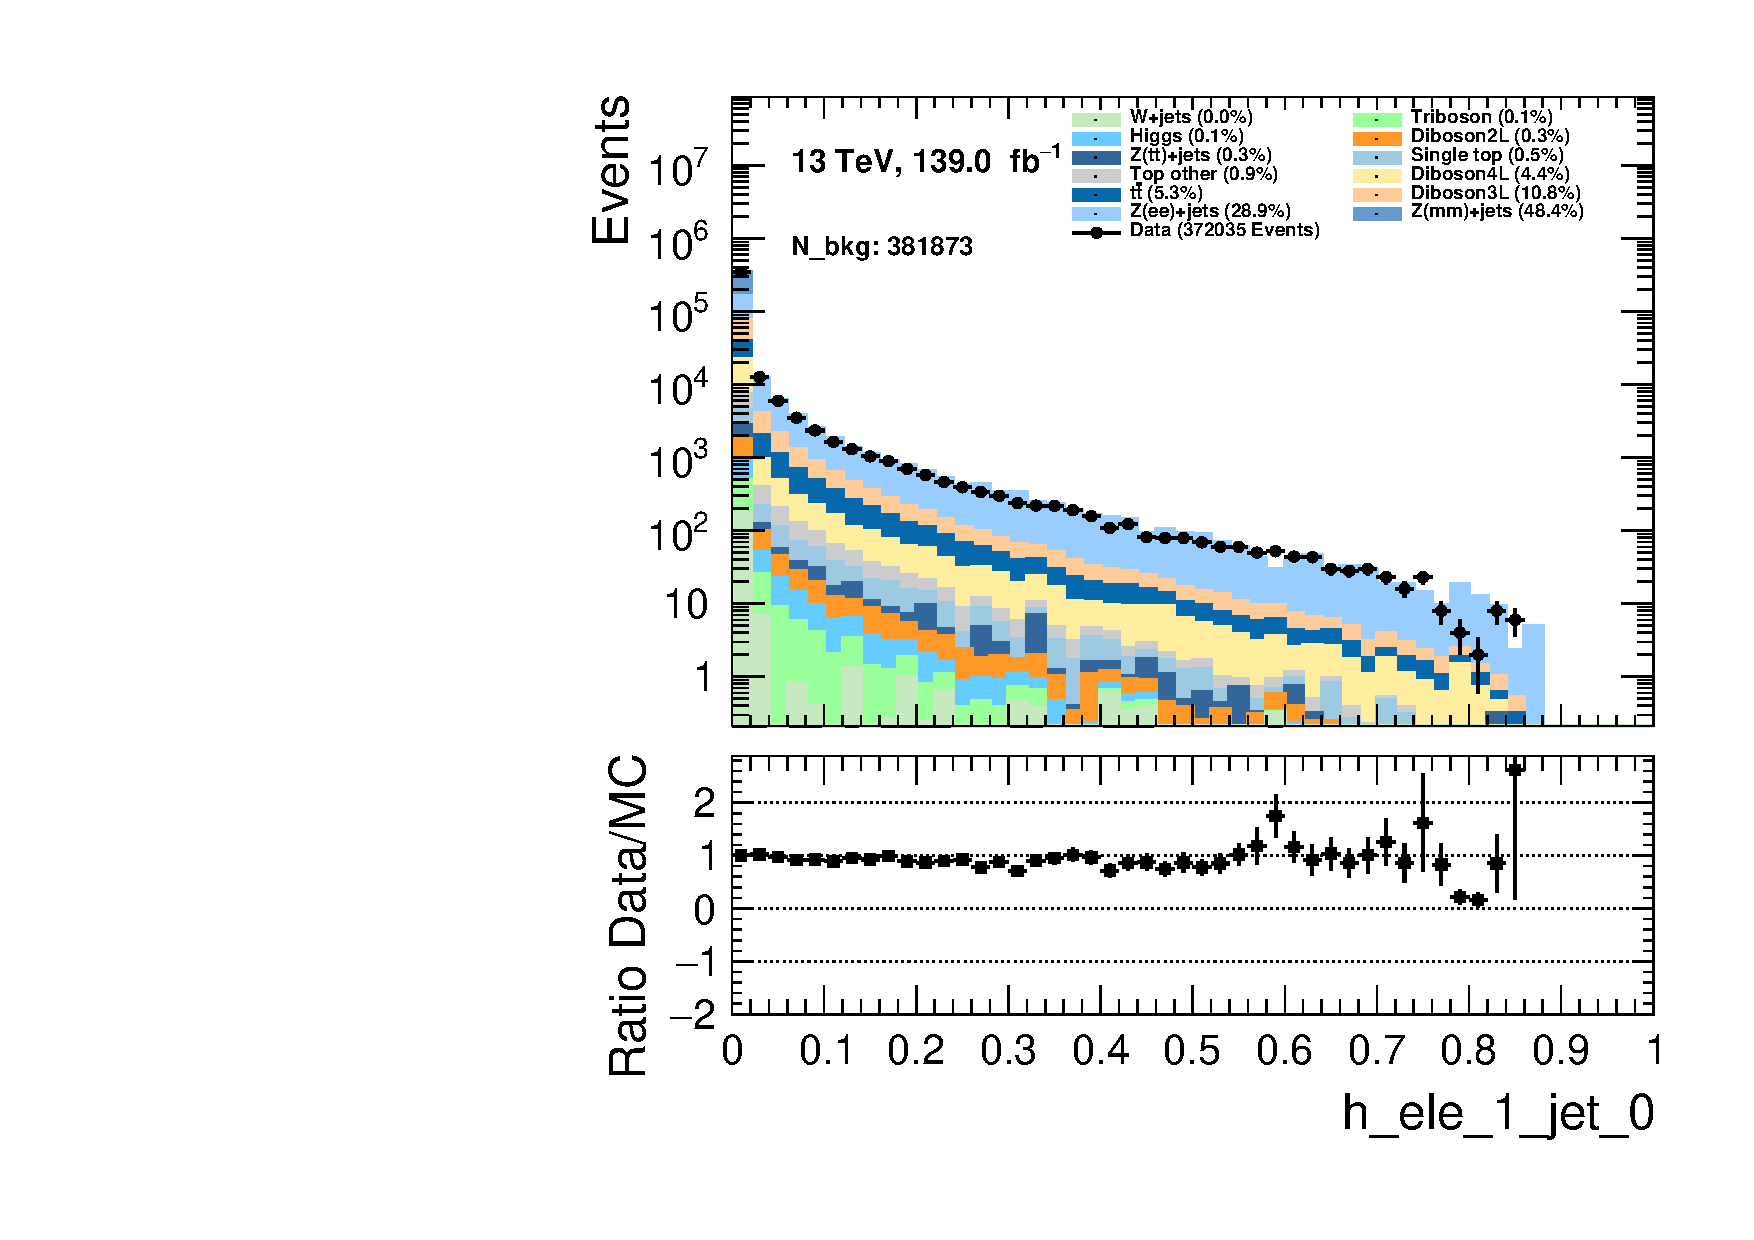
\includegraphics[width=\textwidth]{Figures/MC_Data_comp/h_ele_1_jet_0.pdf}
        \caption{Longitudal component between second electron and first jet.}
        \label{fig:h_ele_1_jet_0}
    \end{subfigure}
    \hfill
    \begin{subfigure}{.49\textwidth}
        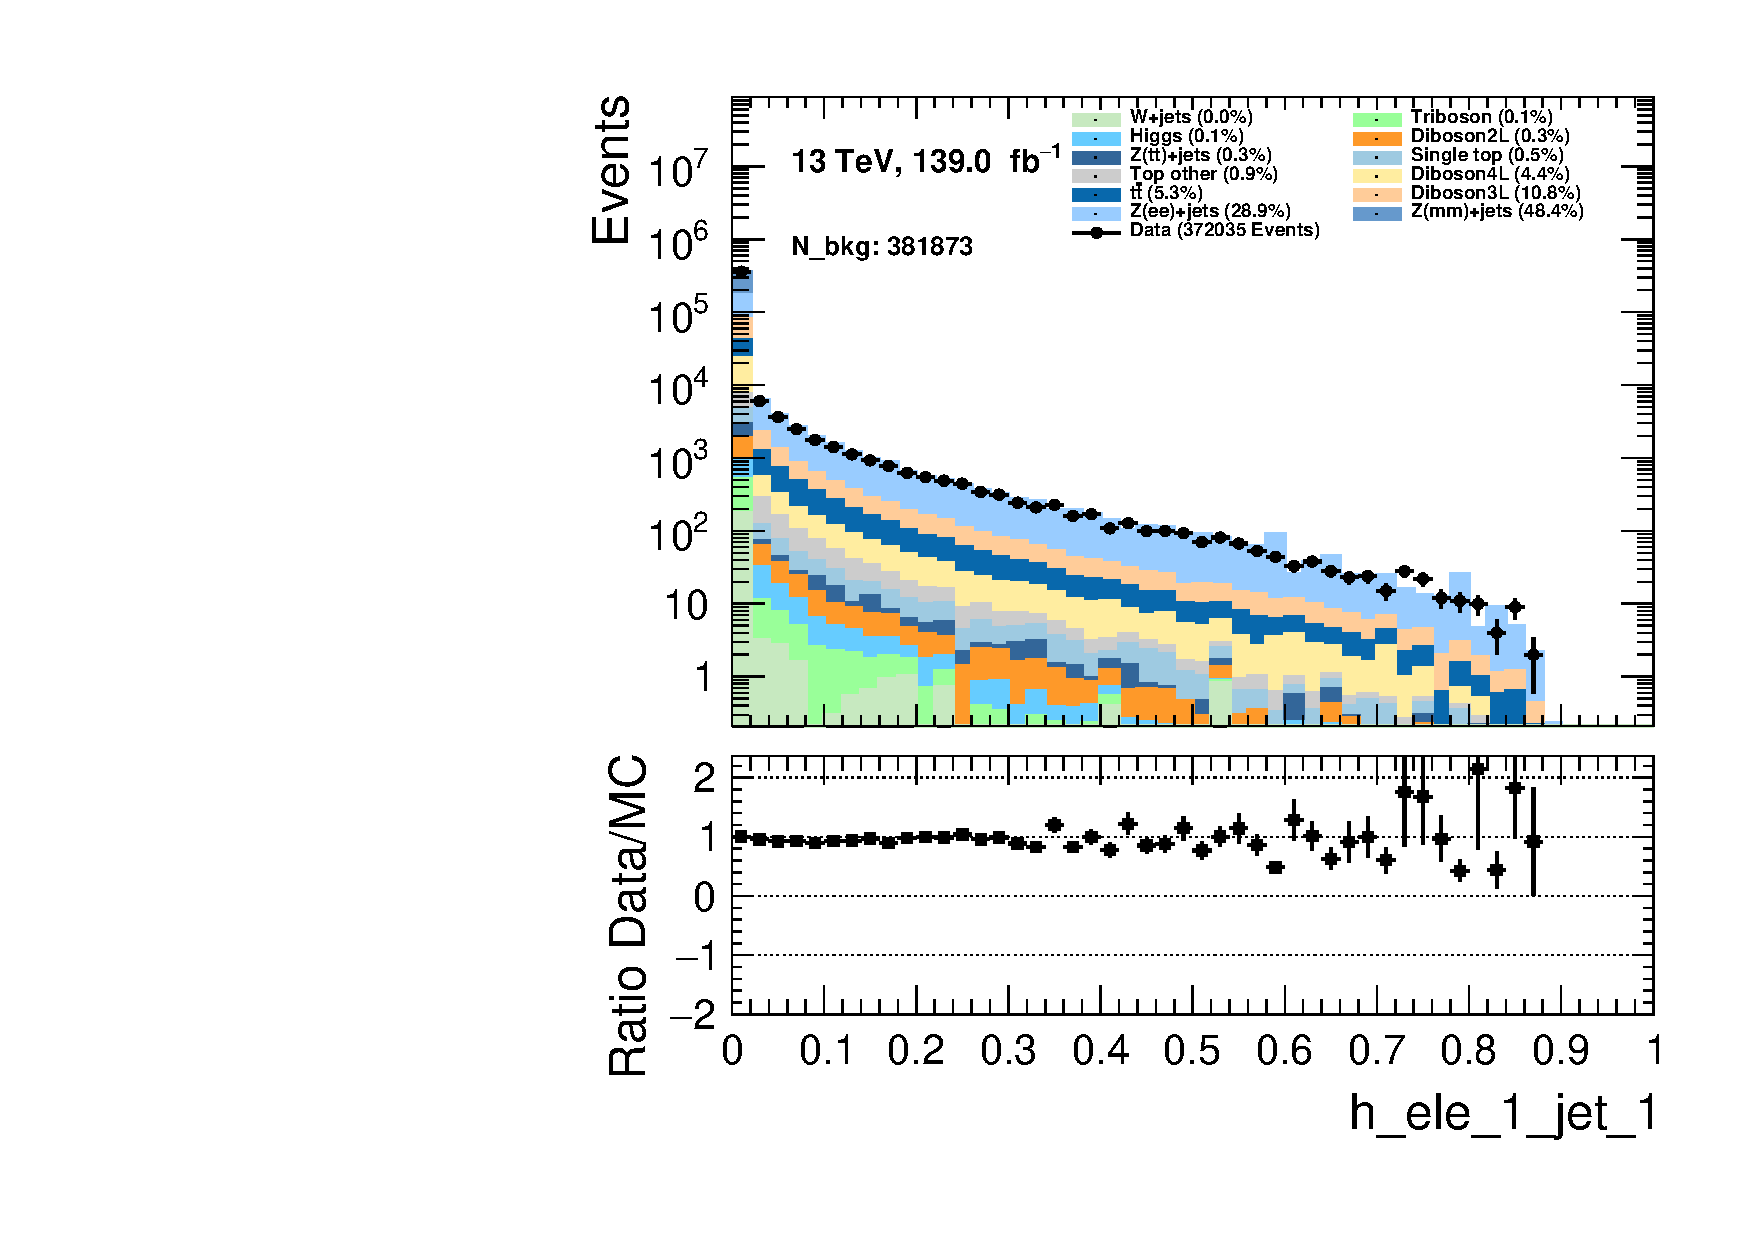
\includegraphics[width=\textwidth]{Figures/MC_Data_comp/h_ele_1_jet_1.pdf}
        \caption{Longitudal component between second electron and second jet. }
        \label{fig:h_ele_1_jet_1}
    \end{subfigure}
    \hfill       
    \caption{Longitudal components between electrons and electrons, and electrons and jets.}
    \label{fig:batch4_feats}
\end{figure}

\begin{figure}
    \centering
    \begin{subfigure}{.49\textwidth}
        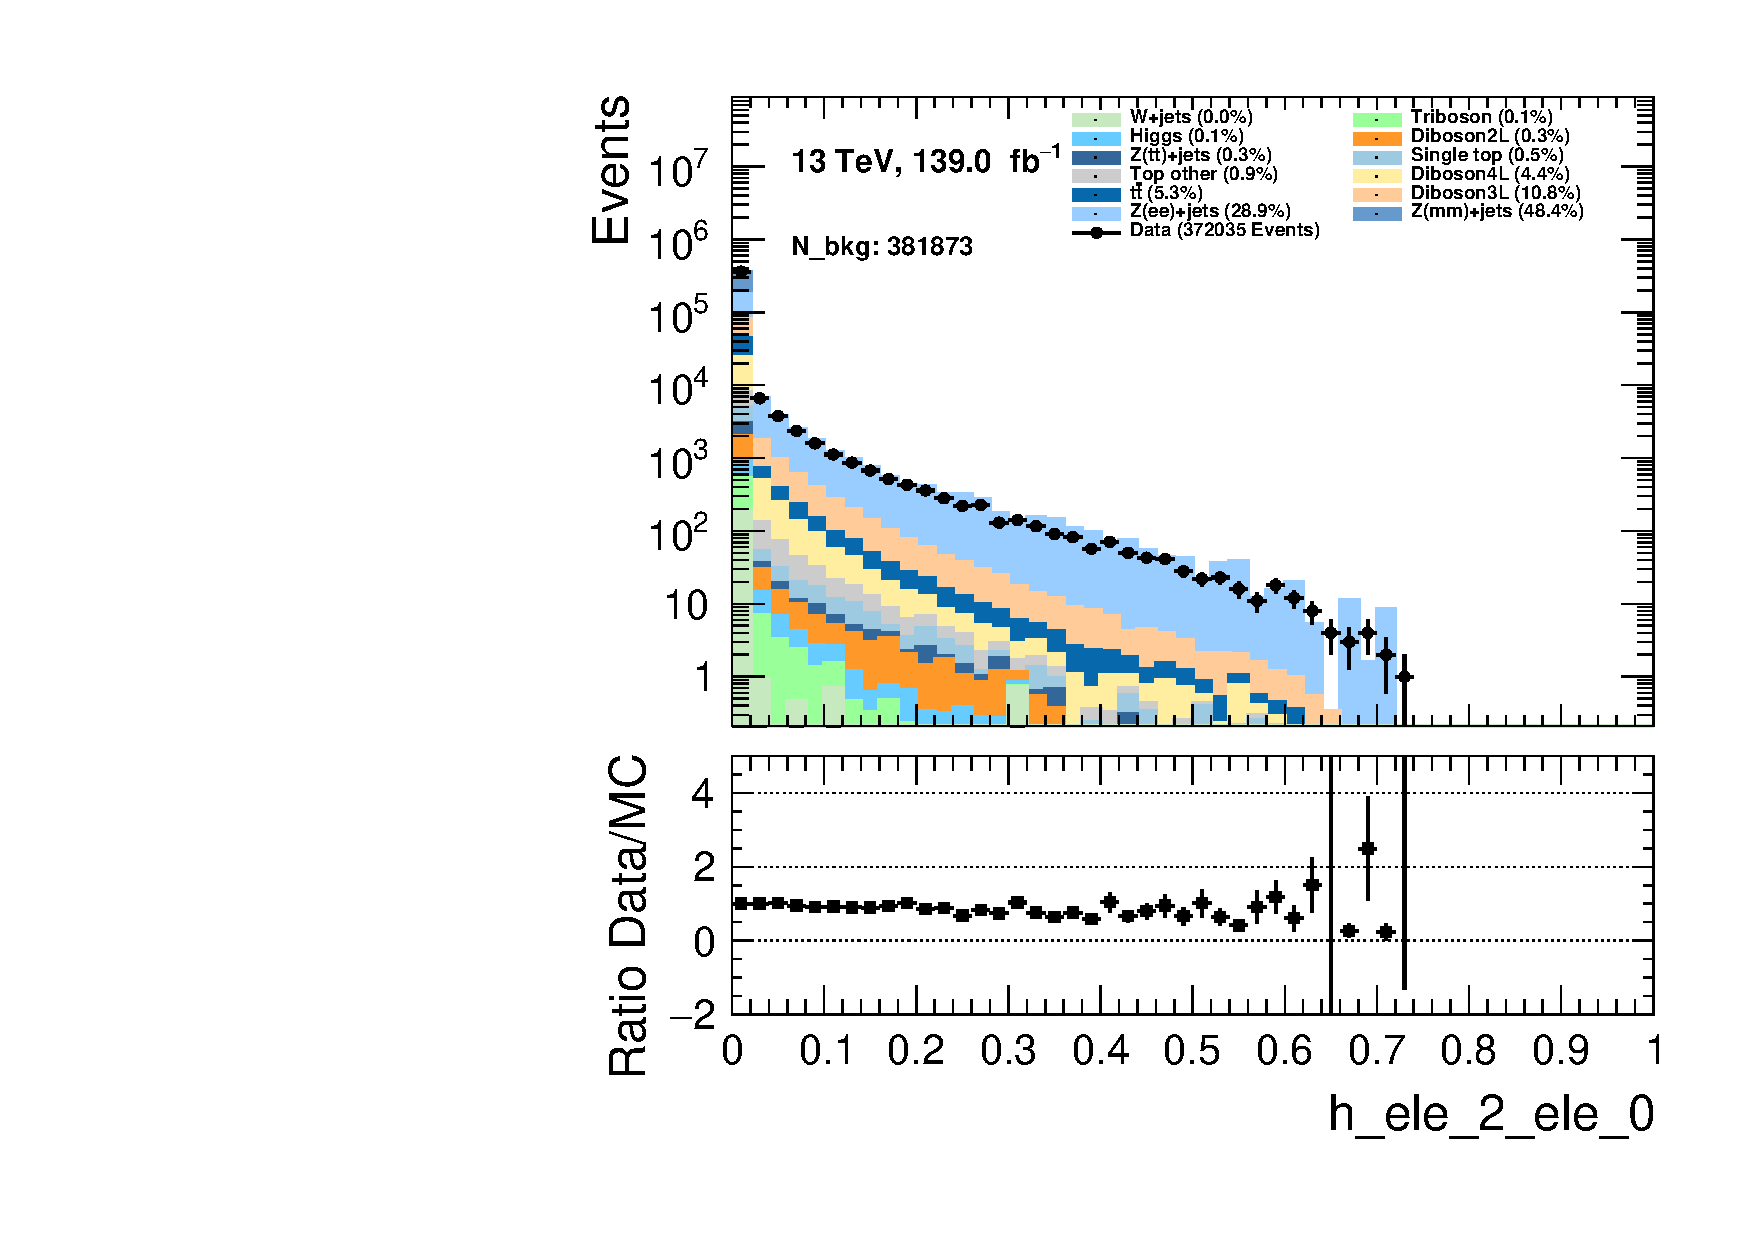
\includegraphics[width=\textwidth]{Figures/MC_Data_comp/h_ele_2_ele_0.pdf}
        \caption{Longitudal component between first and third electron.}
        \label{fig:h_ele_2_ele_0}
    \end{subfigure}
    \hfill
    \begin{subfigure}{.49\textwidth}
        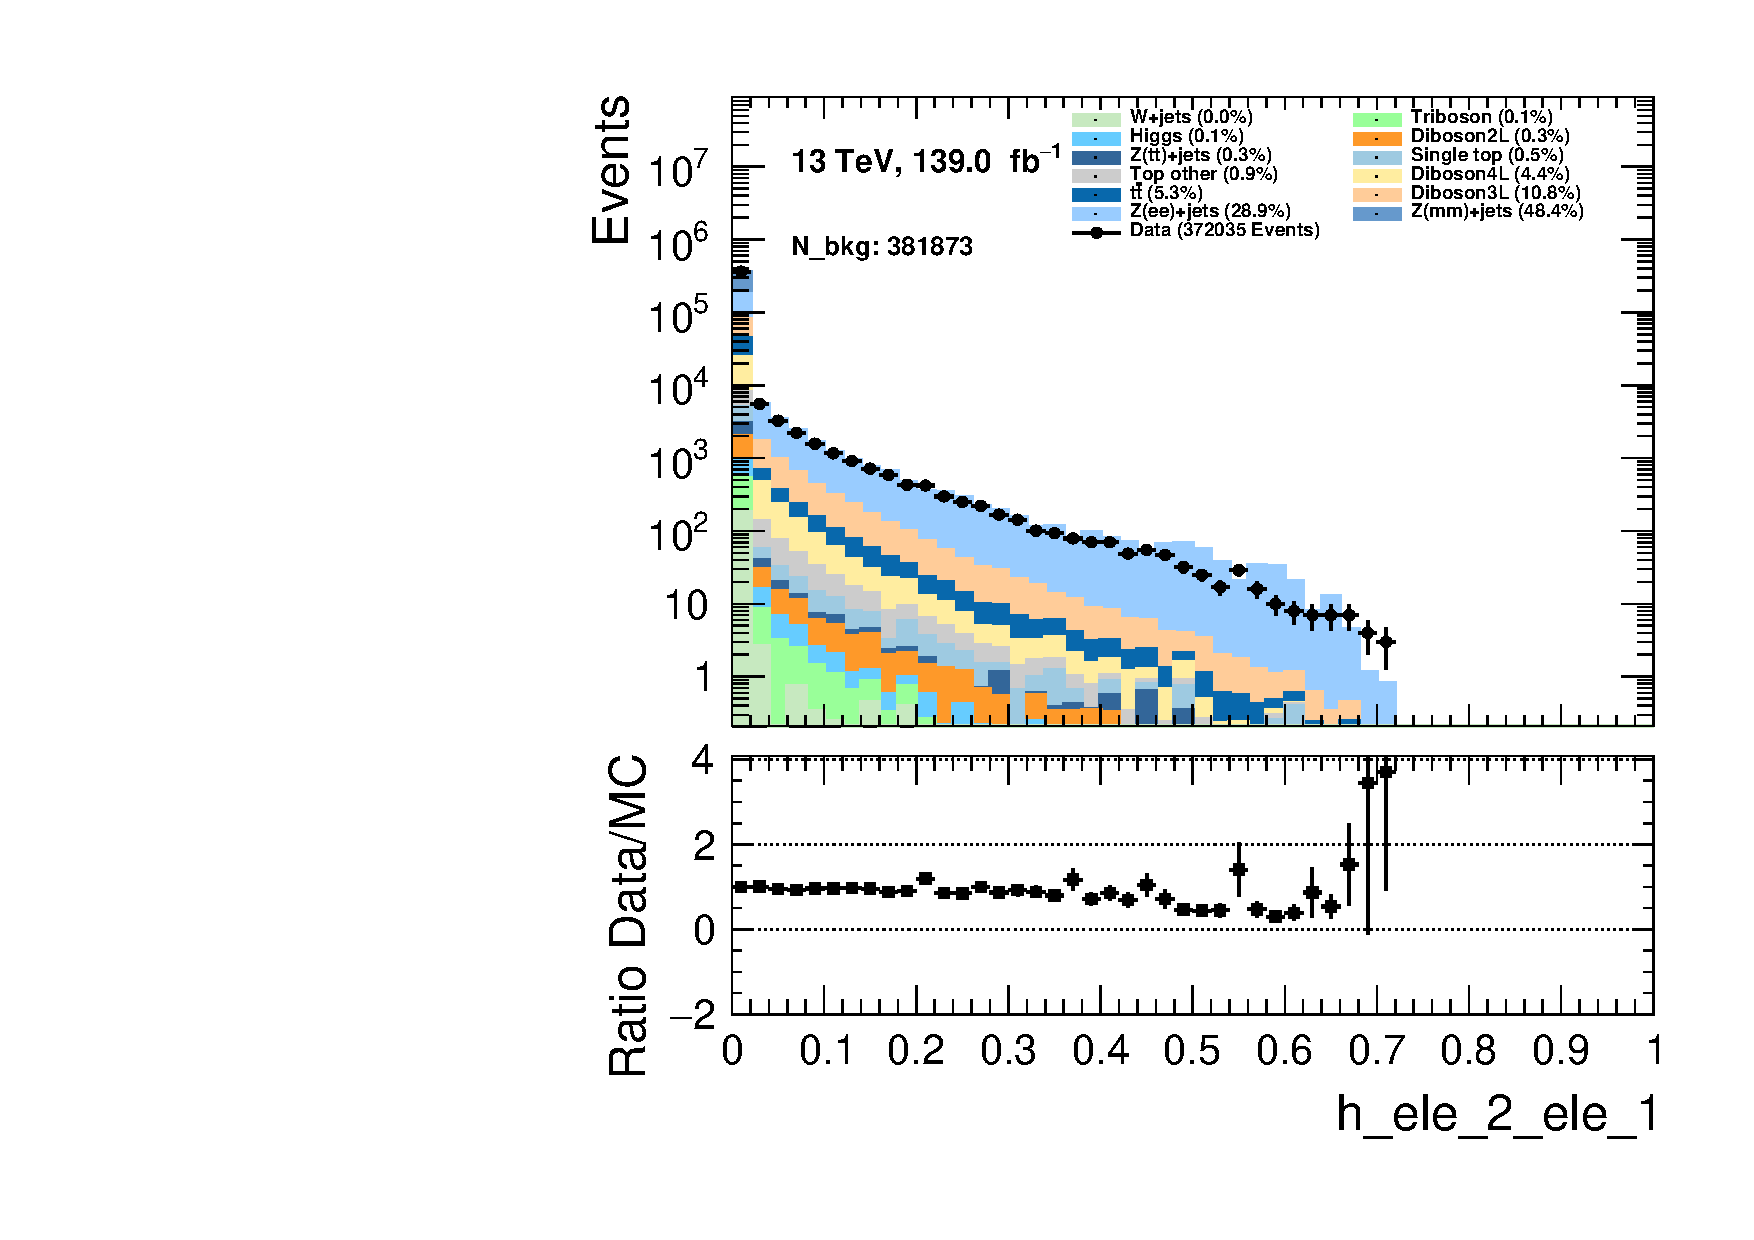
\includegraphics[width=\textwidth]{Figures/MC_Data_comp/h_ele_2_ele_1.pdf}
        \caption{Longitudal component between second and third electron. }
        \label{fig:h_ele_2_ele_1}
    \end{subfigure}
    \hfill 
    \begin{subfigure}{.49\textwidth}
        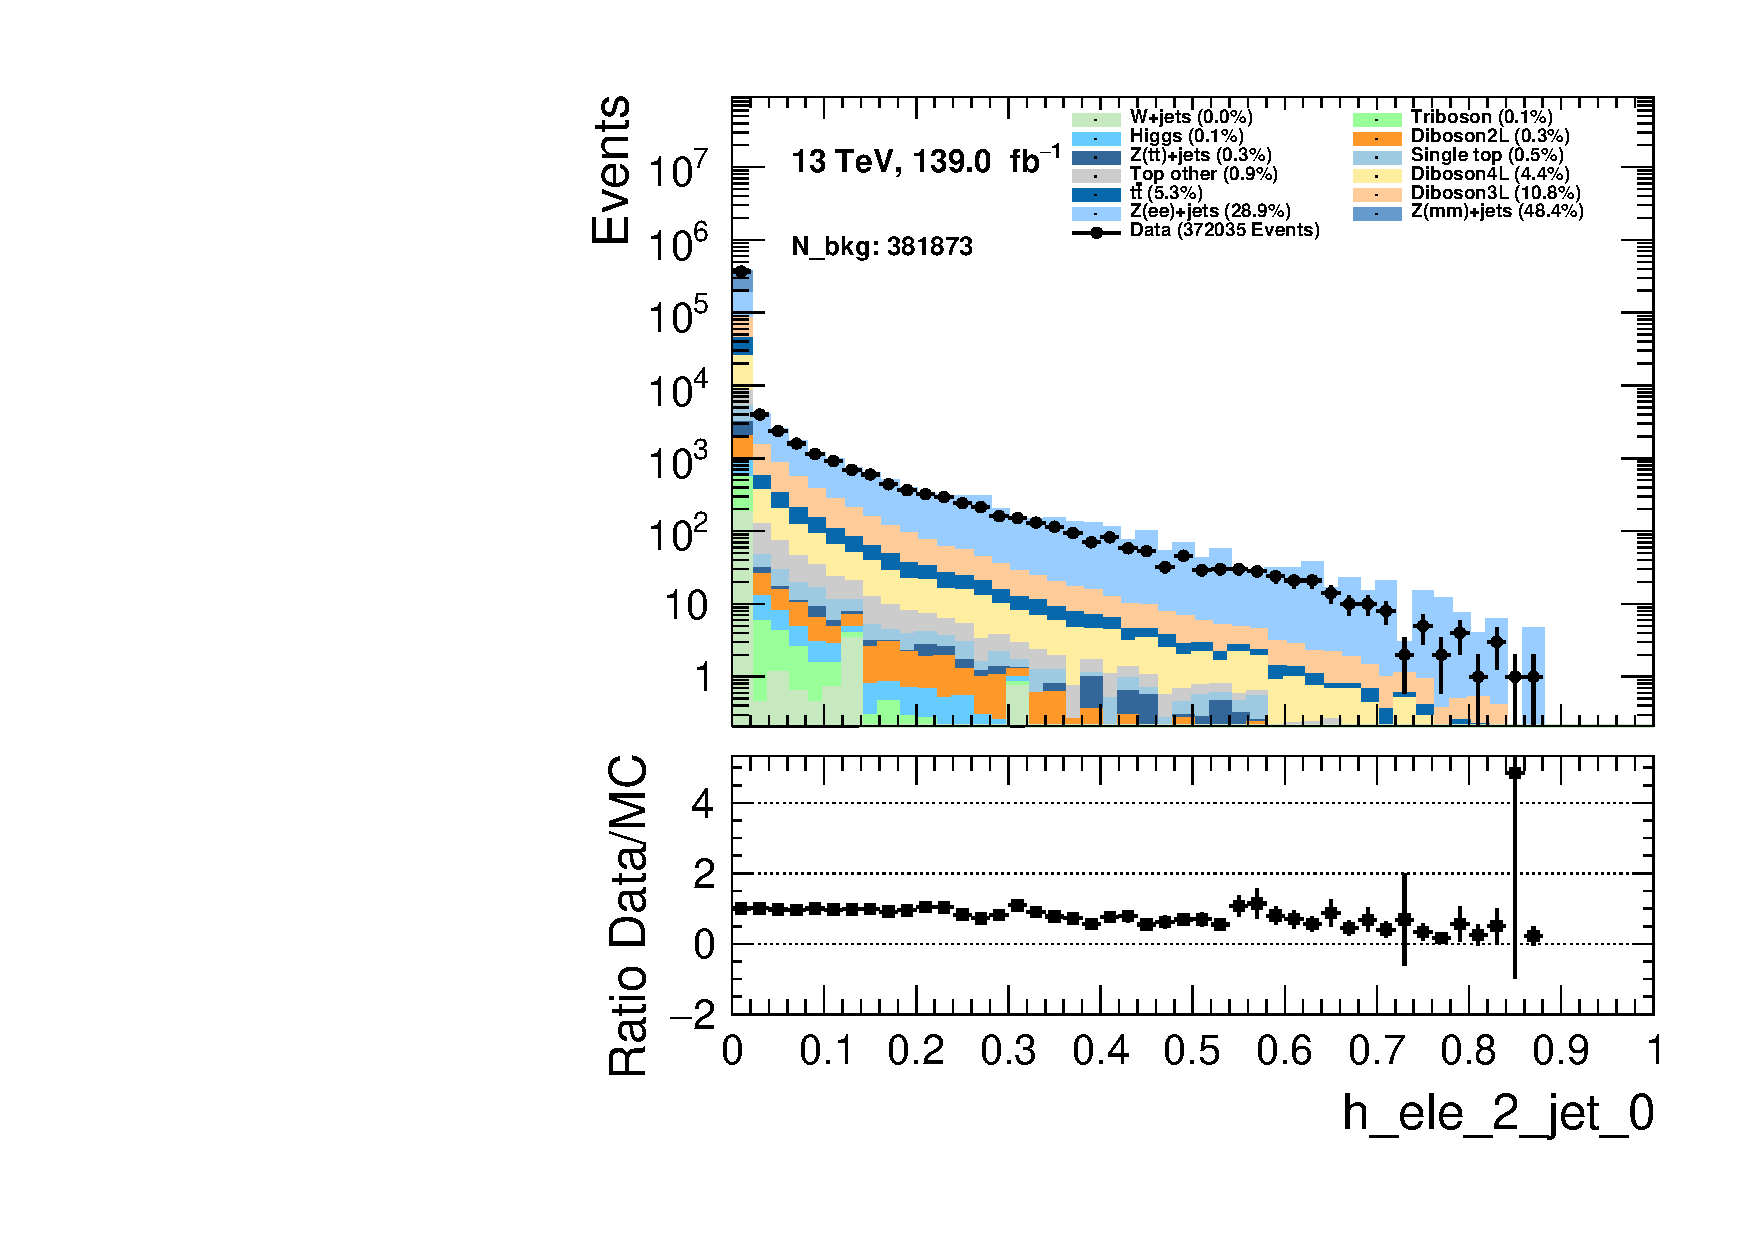
\includegraphics[width=\textwidth]{Figures/MC_Data_comp/h_ele_2_jet_0.pdf}
        \caption{ Longitudal component between third electron and first jet.}
        \label{fig:h_ele_2_jet_0}
    \end{subfigure}
    \hfill
    \begin{subfigure}{.49\textwidth}
        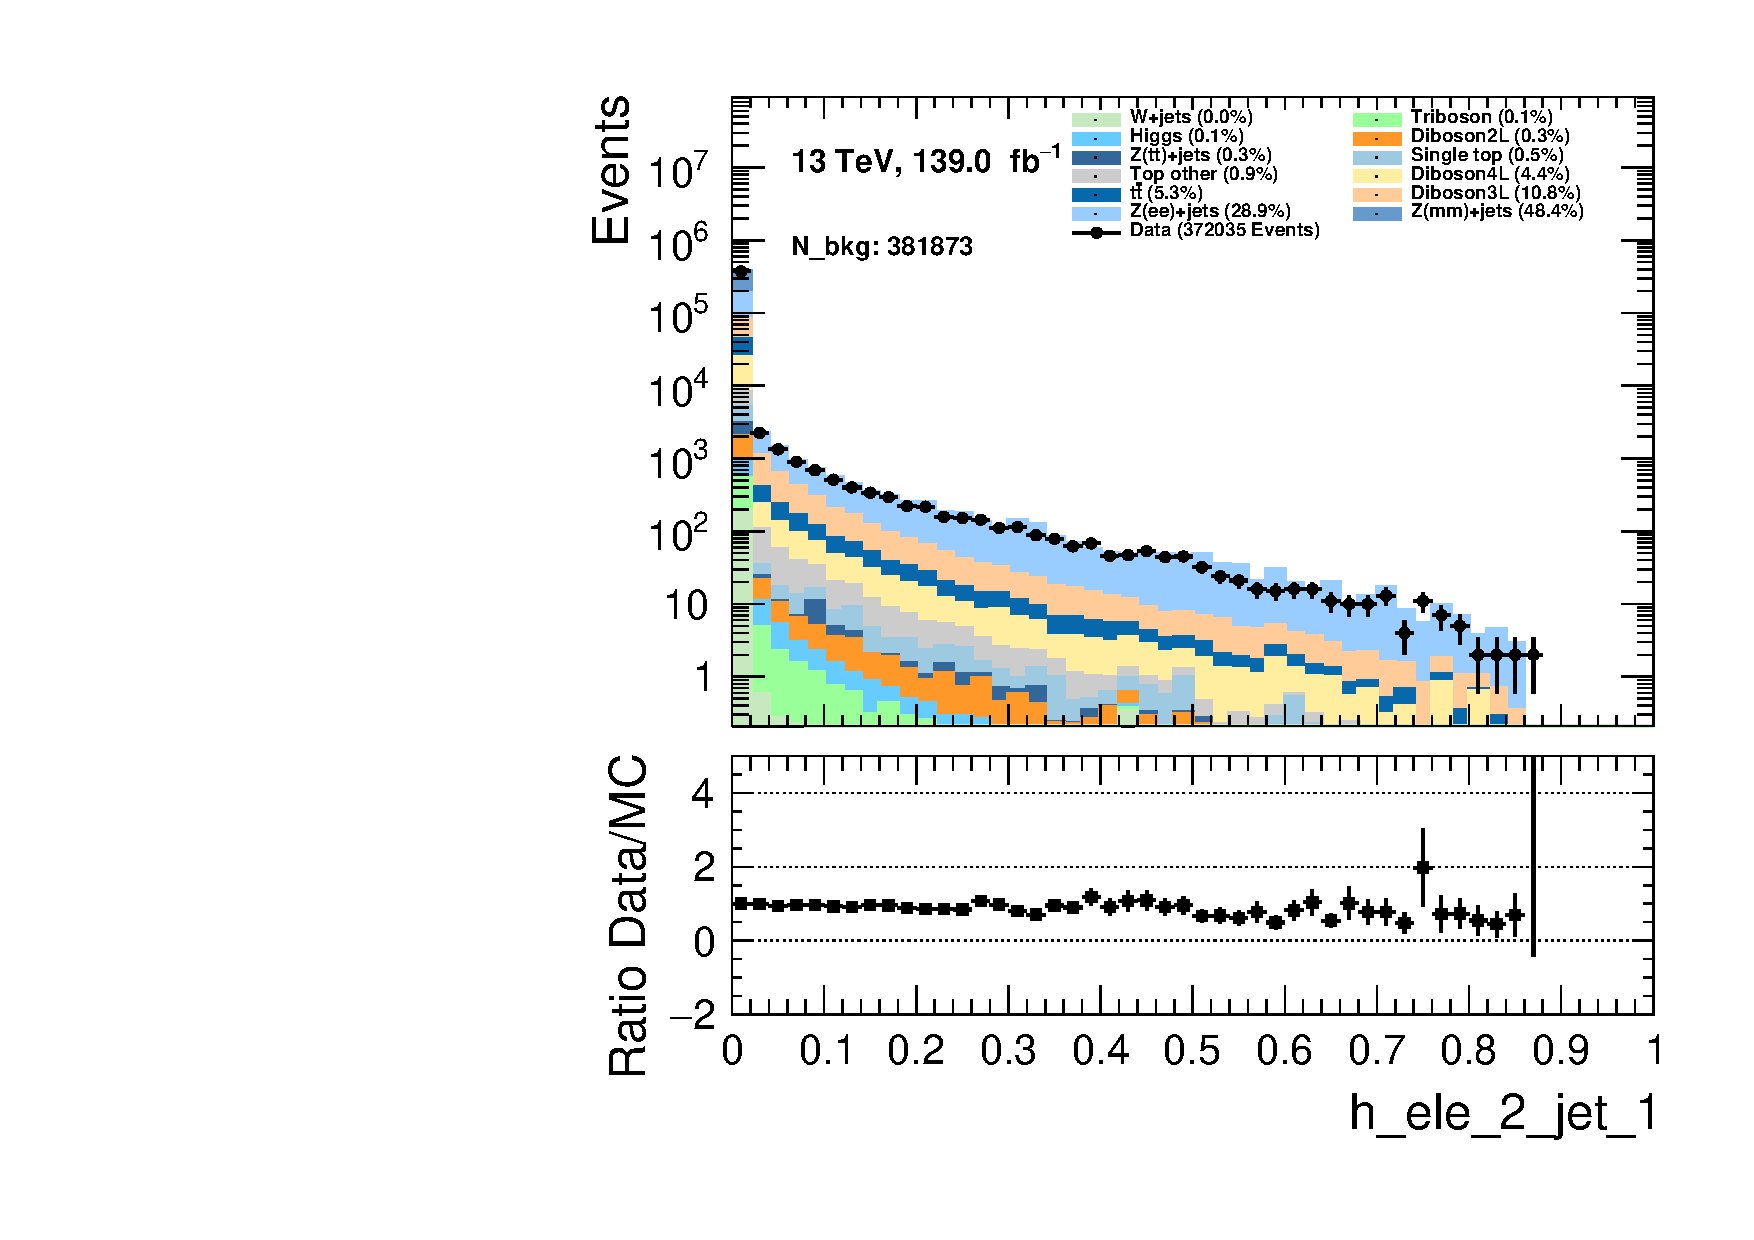
\includegraphics[width=\textwidth]{Figures/MC_Data_comp/h_ele_2_jet_1.pdf}
        \caption{ Longitudal component between third electron and second jet.}
        \label{fig:h_ele_2_jet_1}
    \end{subfigure}
    \hfill       
    \caption{Longitudal component between between electrons and electrons, and electrons and jets.}
    \label{fig:batch5_feats}
\end{figure}

\begin{figure}
    \centering
    \begin{subfigure}{.49\textwidth}
        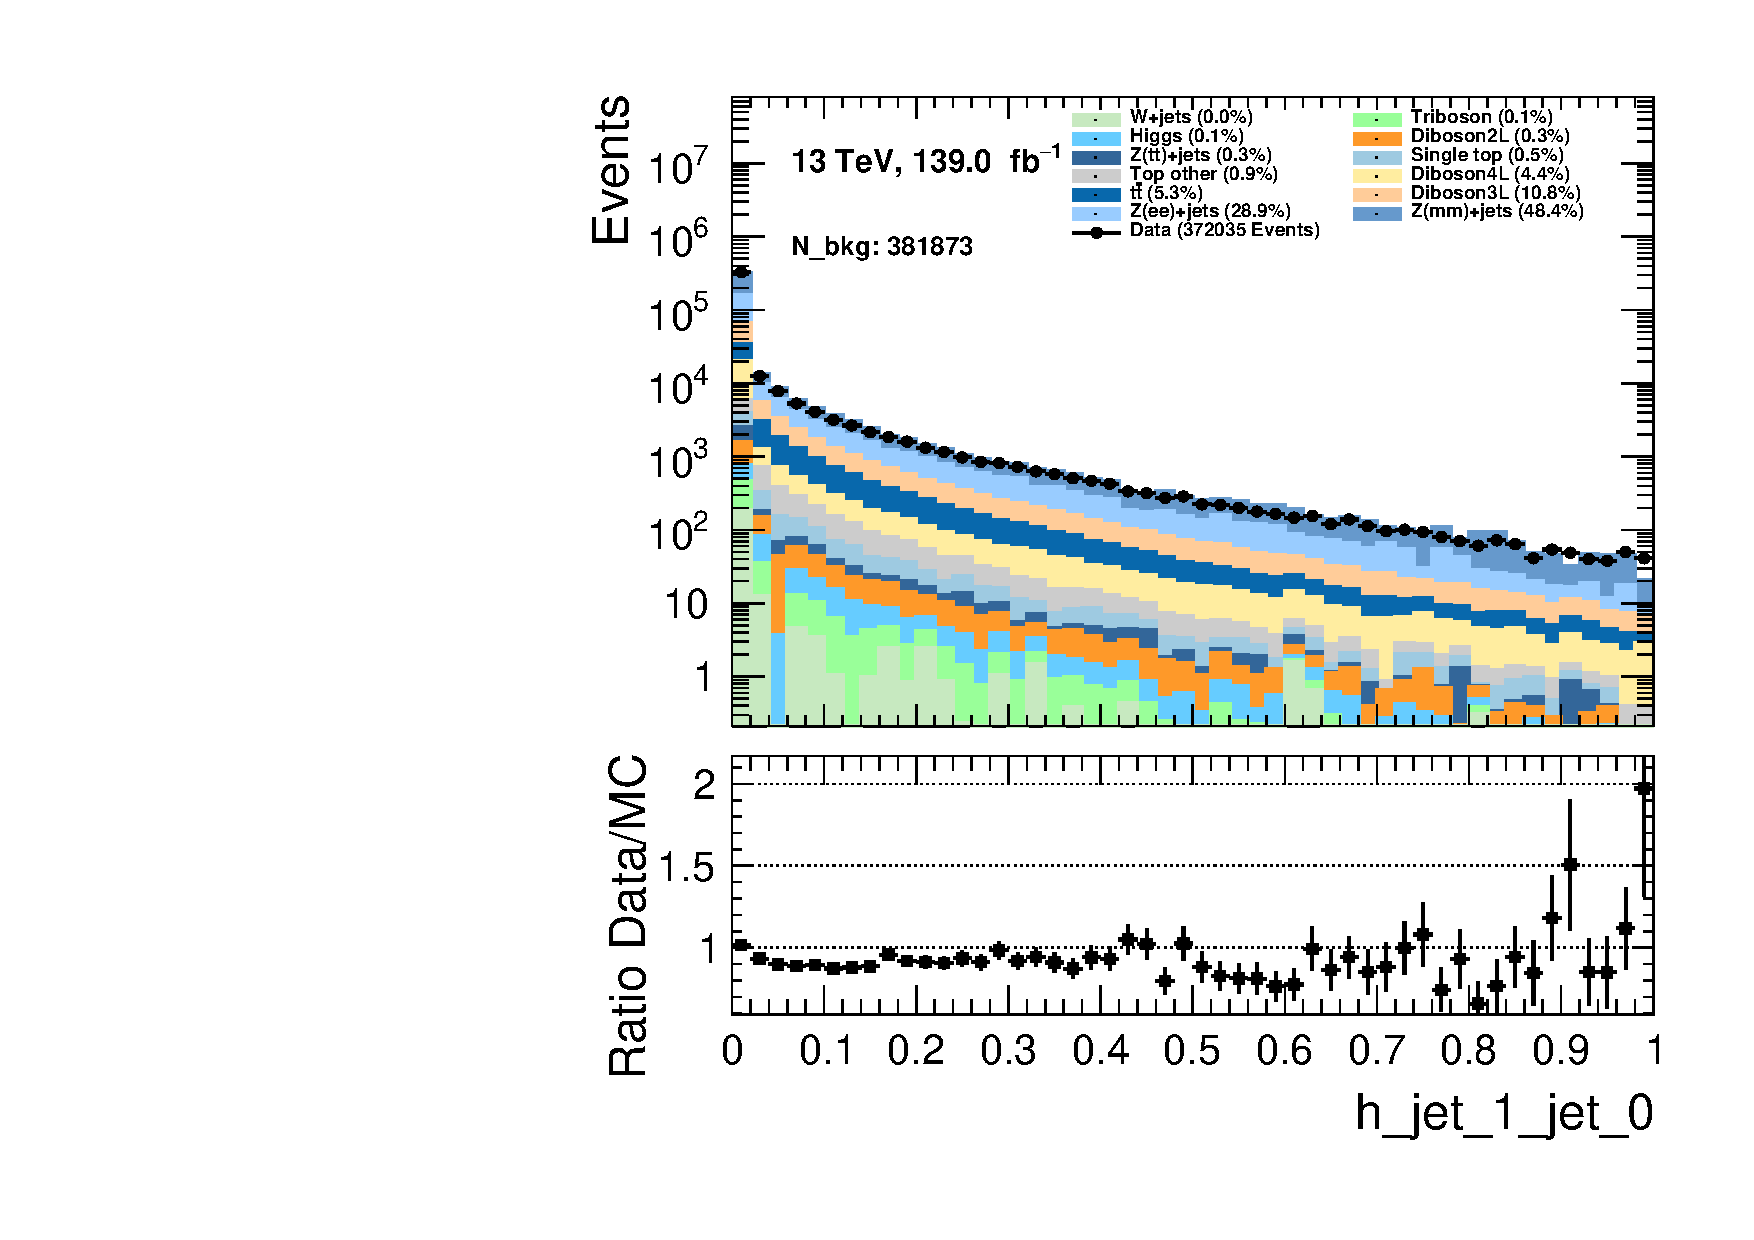
\includegraphics[width=\textwidth]{Figures/MC_Data_comp/h_jet_1_jet_0.pdf}
        \caption{Longitudal component between first and second jet.}
        \label{fig:h_jet_1_jet_0}
    \end{subfigure}
    \hfill
    \begin{subfigure}{.49\textwidth}
        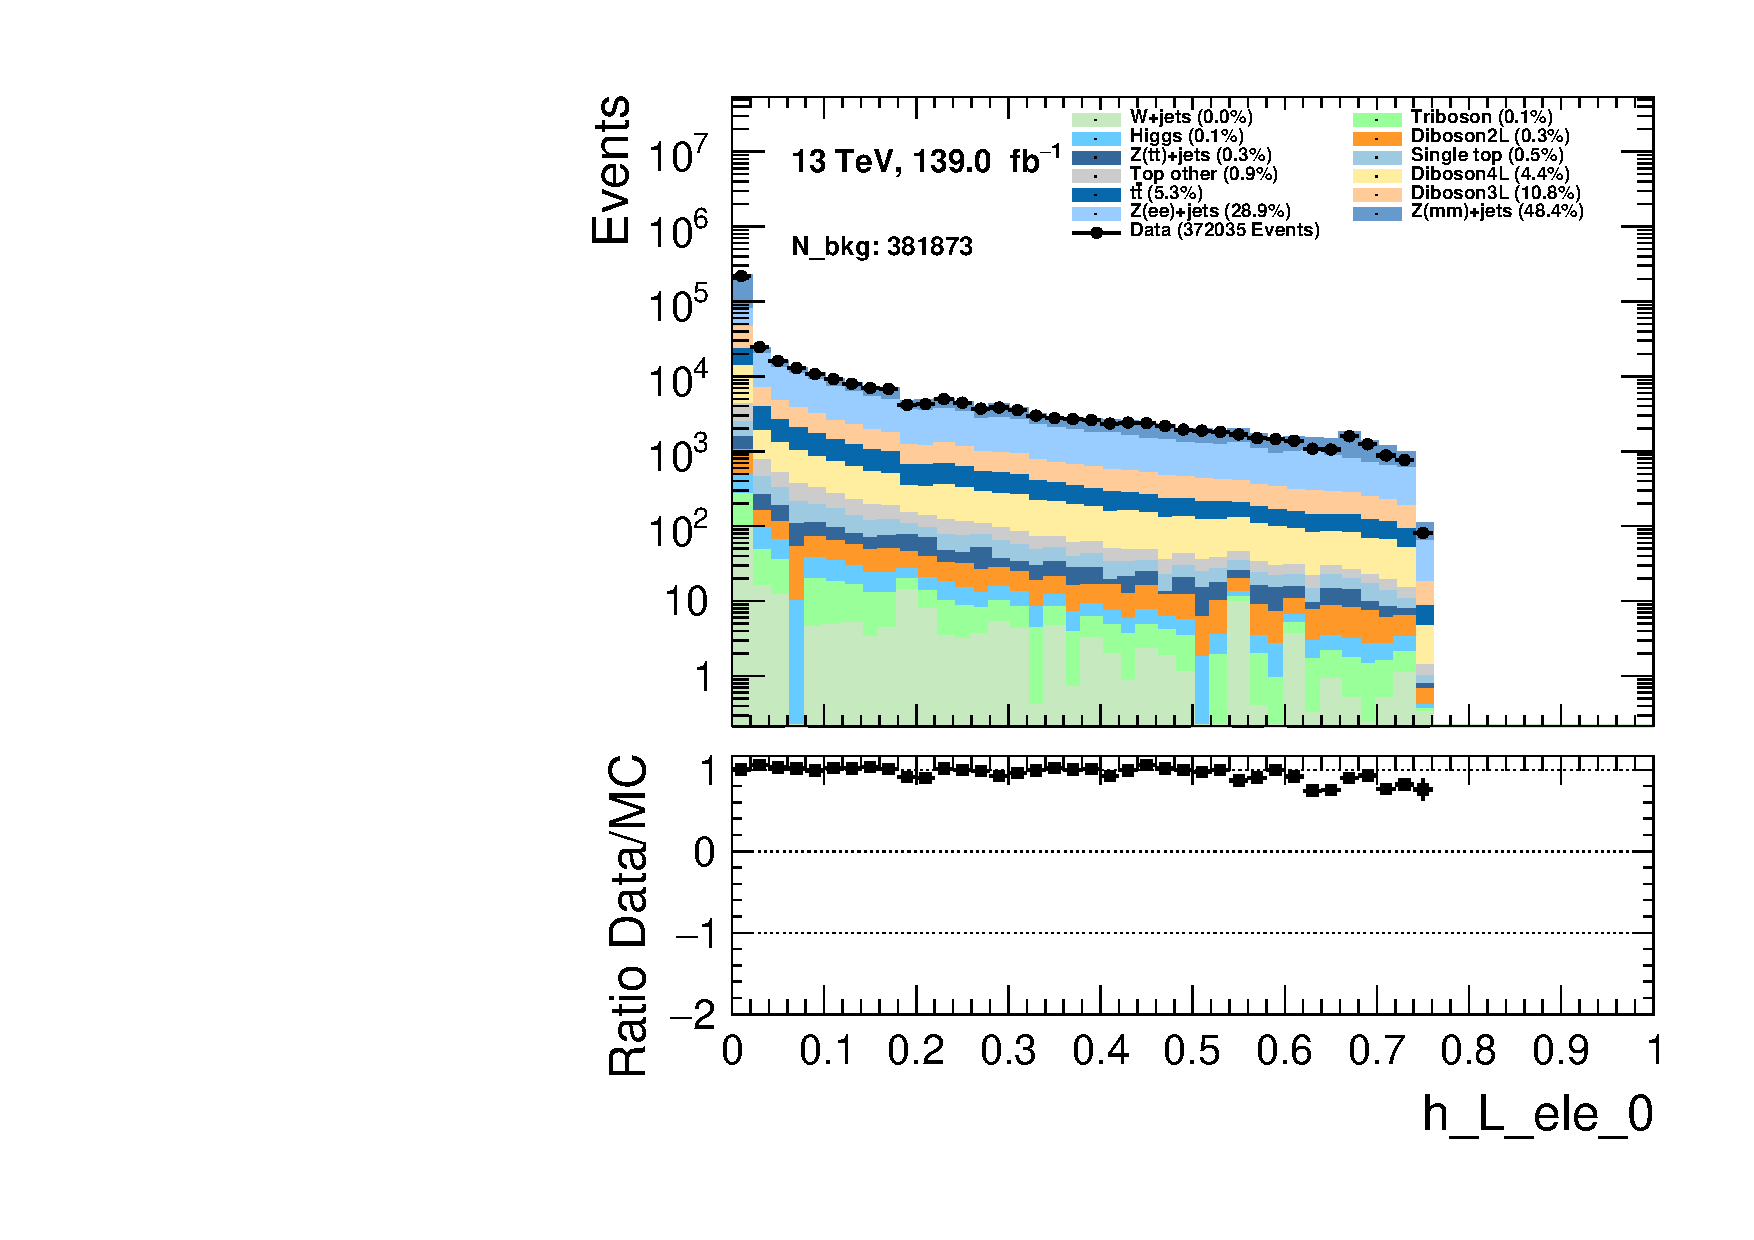
\includegraphics[width=\textwidth]{Figures/MC_Data_comp/h_L_ele_0.pdf}
        \caption{ Longitudal component between for first electron}
        \label{fig:h_L_ele_0}
    \end{subfigure}
    \hfill 
    \begin{subfigure}{.49\textwidth}
        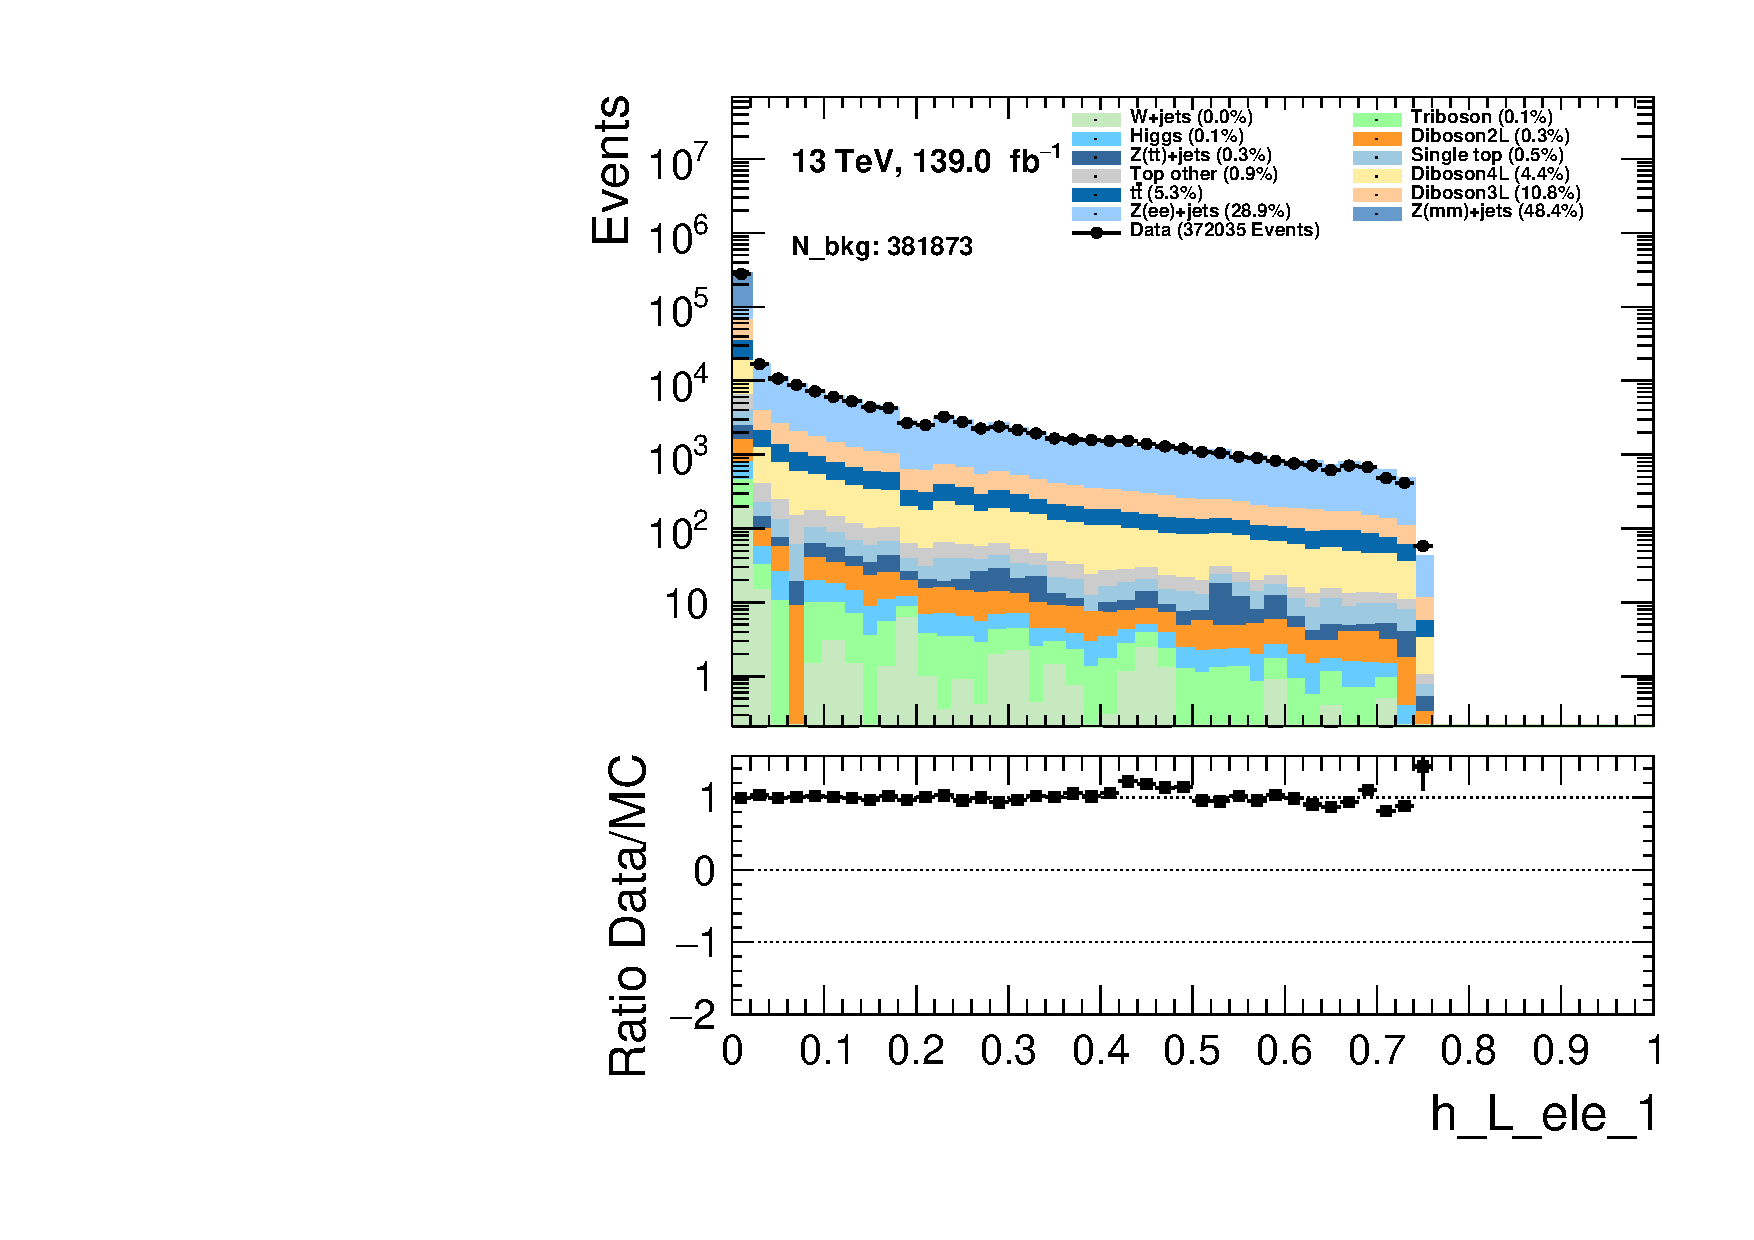
\includegraphics[width=\textwidth]{Figures/MC_Data_comp/h_L_ele_1.pdf}
        \caption{Longitudal component for second electron. }
        \label{fig:h_L_ele_1}
    \end{subfigure}
    \hfill
    \begin{subfigure}{.49\textwidth}
        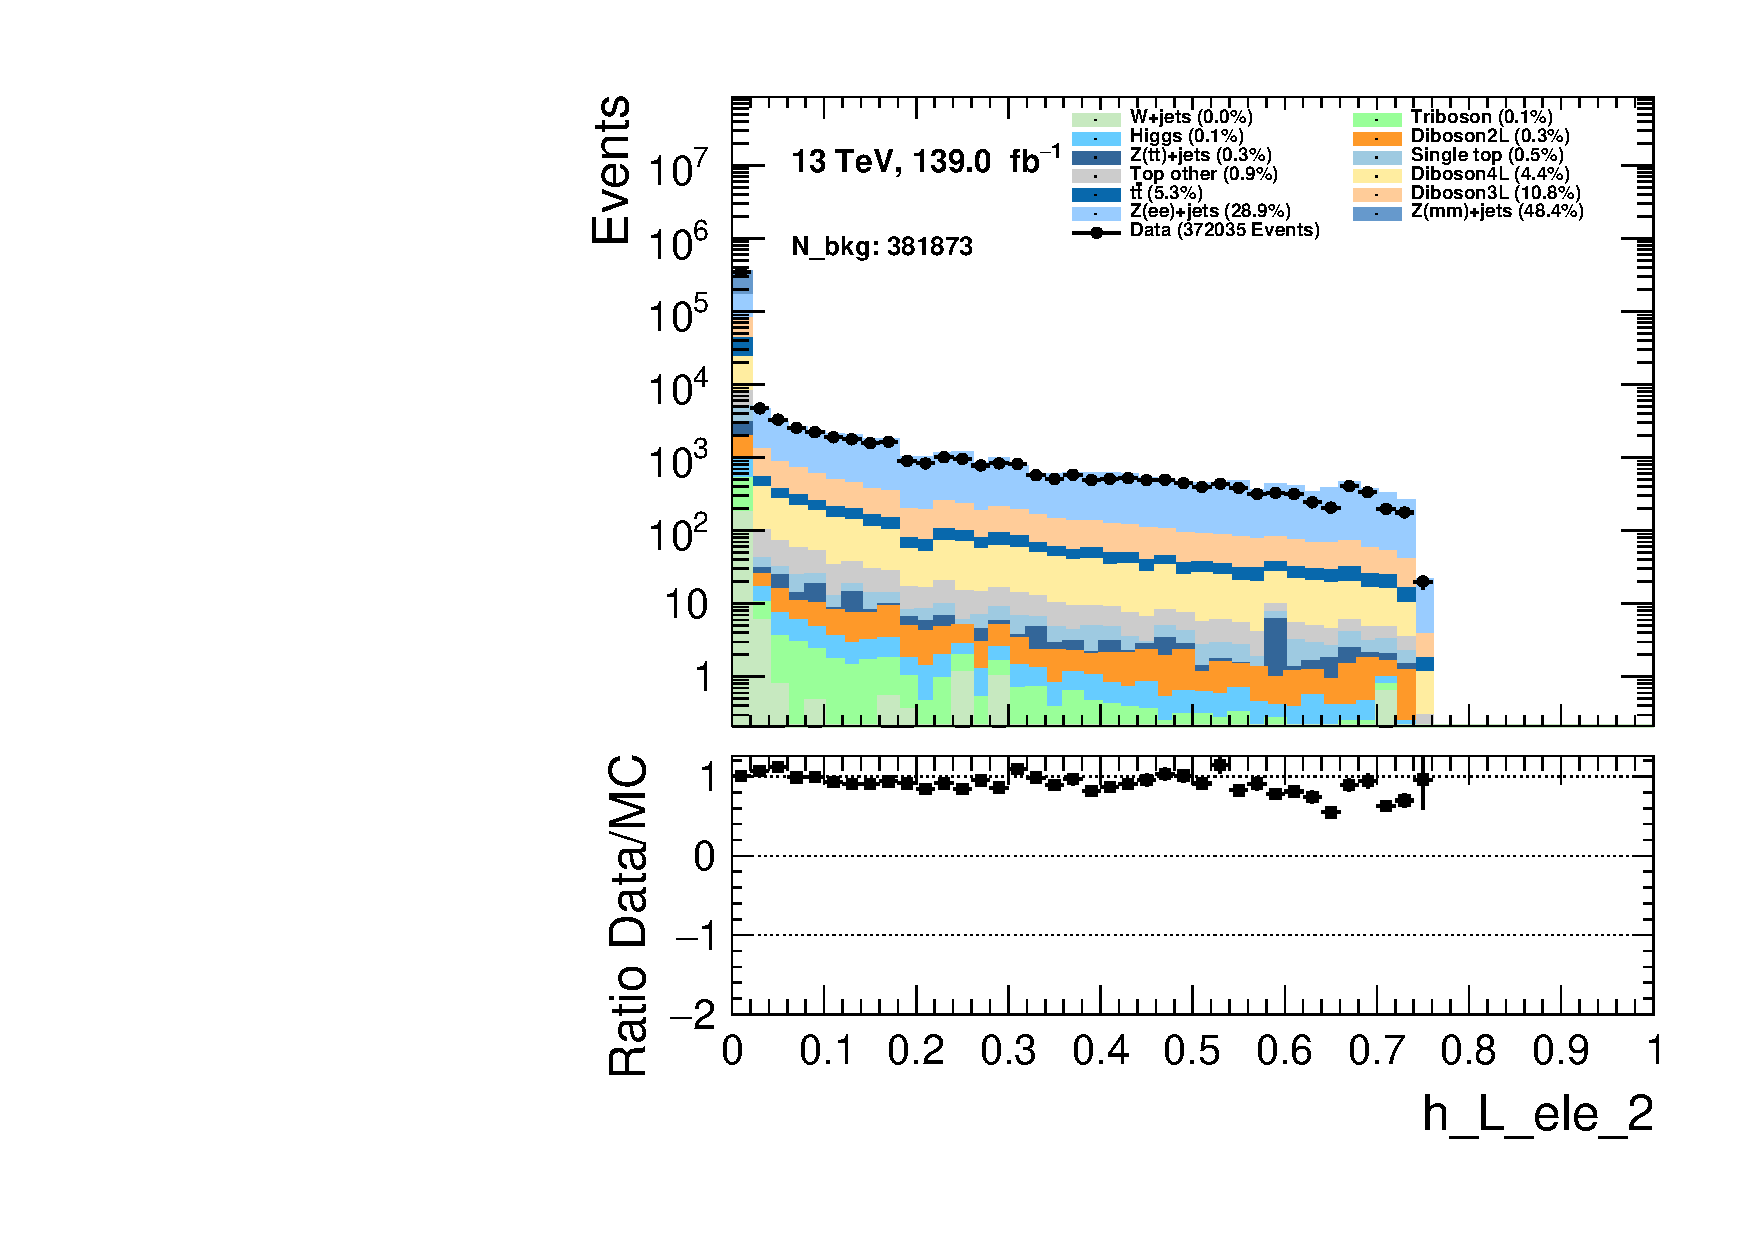
\includegraphics[width=\textwidth]{Figures/MC_Data_comp/h_L_ele_2.pdf}
        \caption{ Longitudal component for third electron.}
        \label{fig:h_L_ele_2}
    \end{subfigure}
    \hfill       
    \caption{Longitudal component between electron and jet, and for individual electrons.}
    \label{fig:batch6_feats}
\end{figure}

\begin{figure}
    \centering
    \begin{subfigure}{.49\textwidth}
        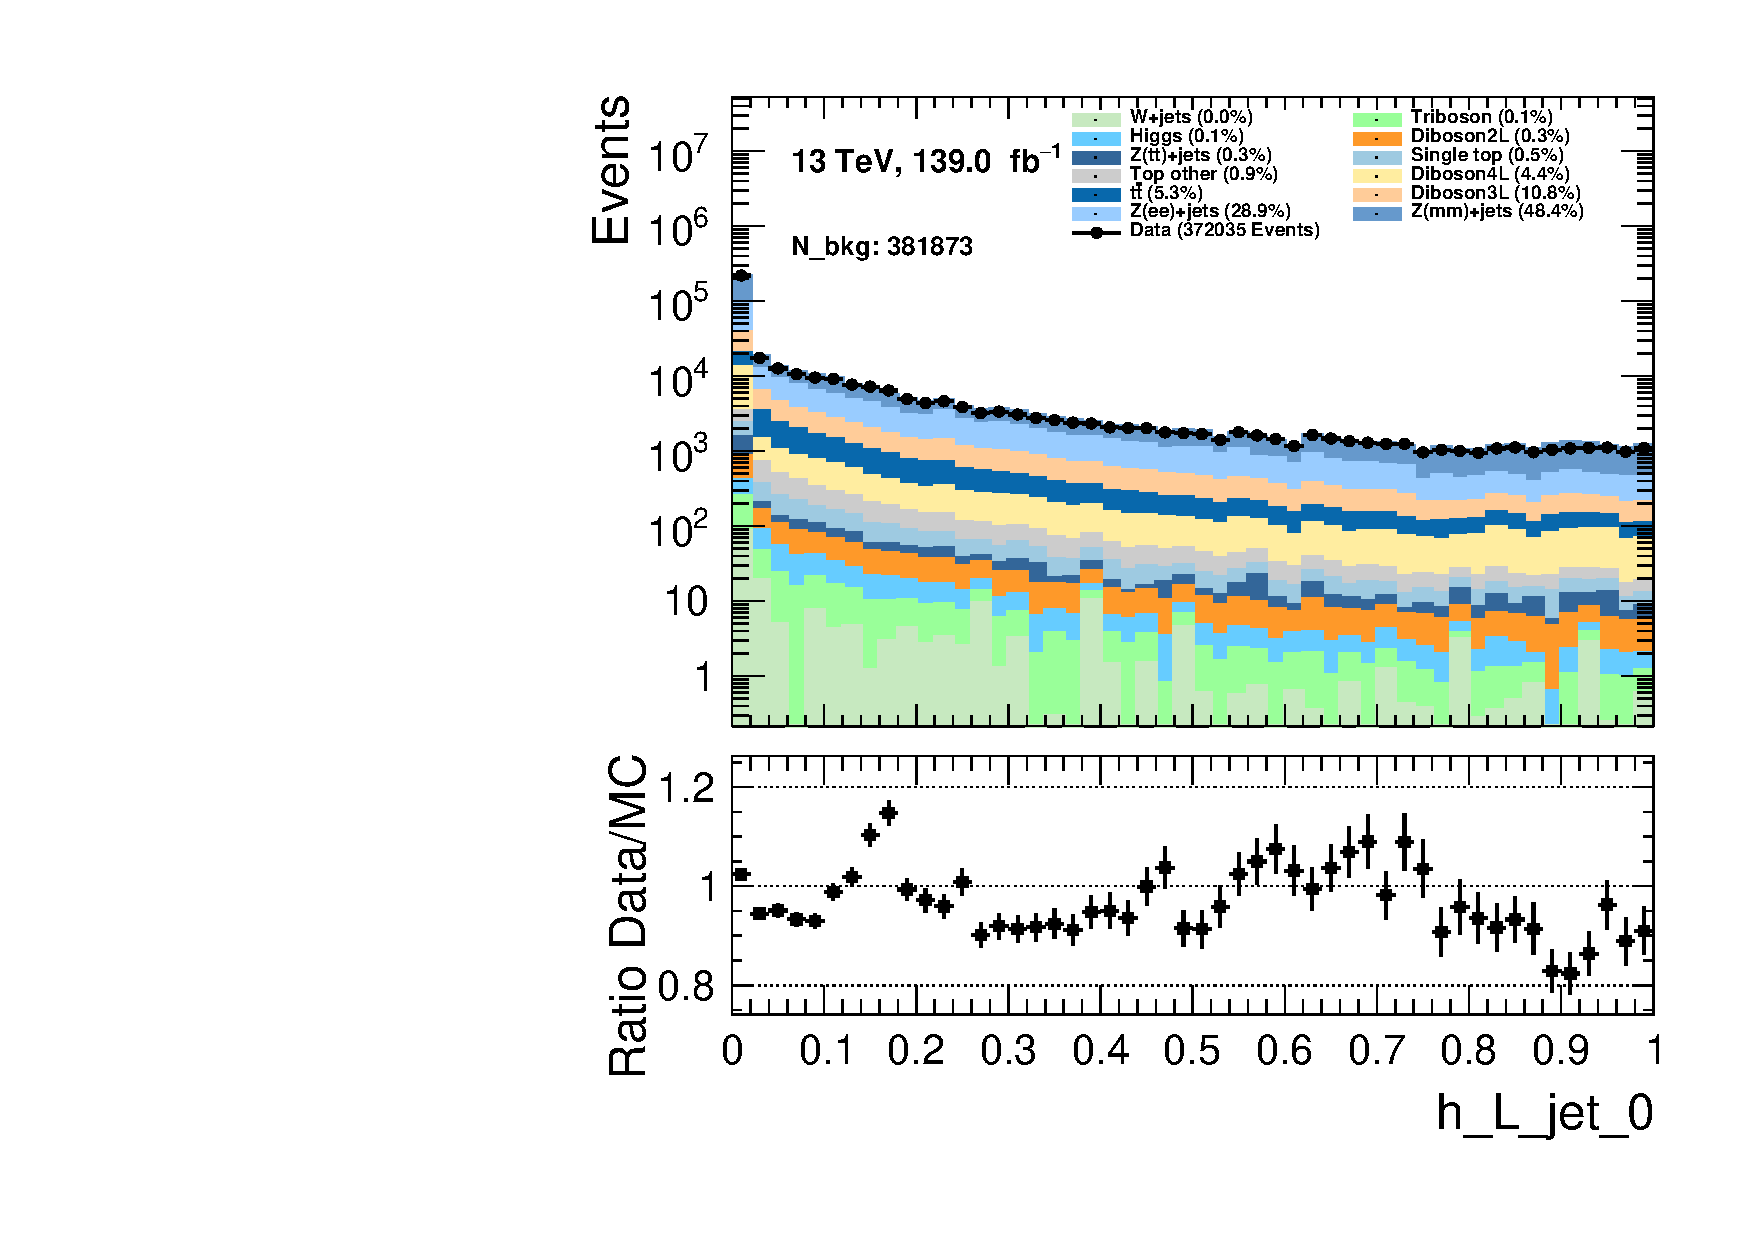
\includegraphics[width=\textwidth]{Figures/MC_Data_comp/h_L_jet_0.pdf}
        \caption{Longitudal component for the first jet.}
        \label{fig:h_L_jet_0}
    \end{subfigure}
    \hfill
    \begin{subfigure}{.49\textwidth}
        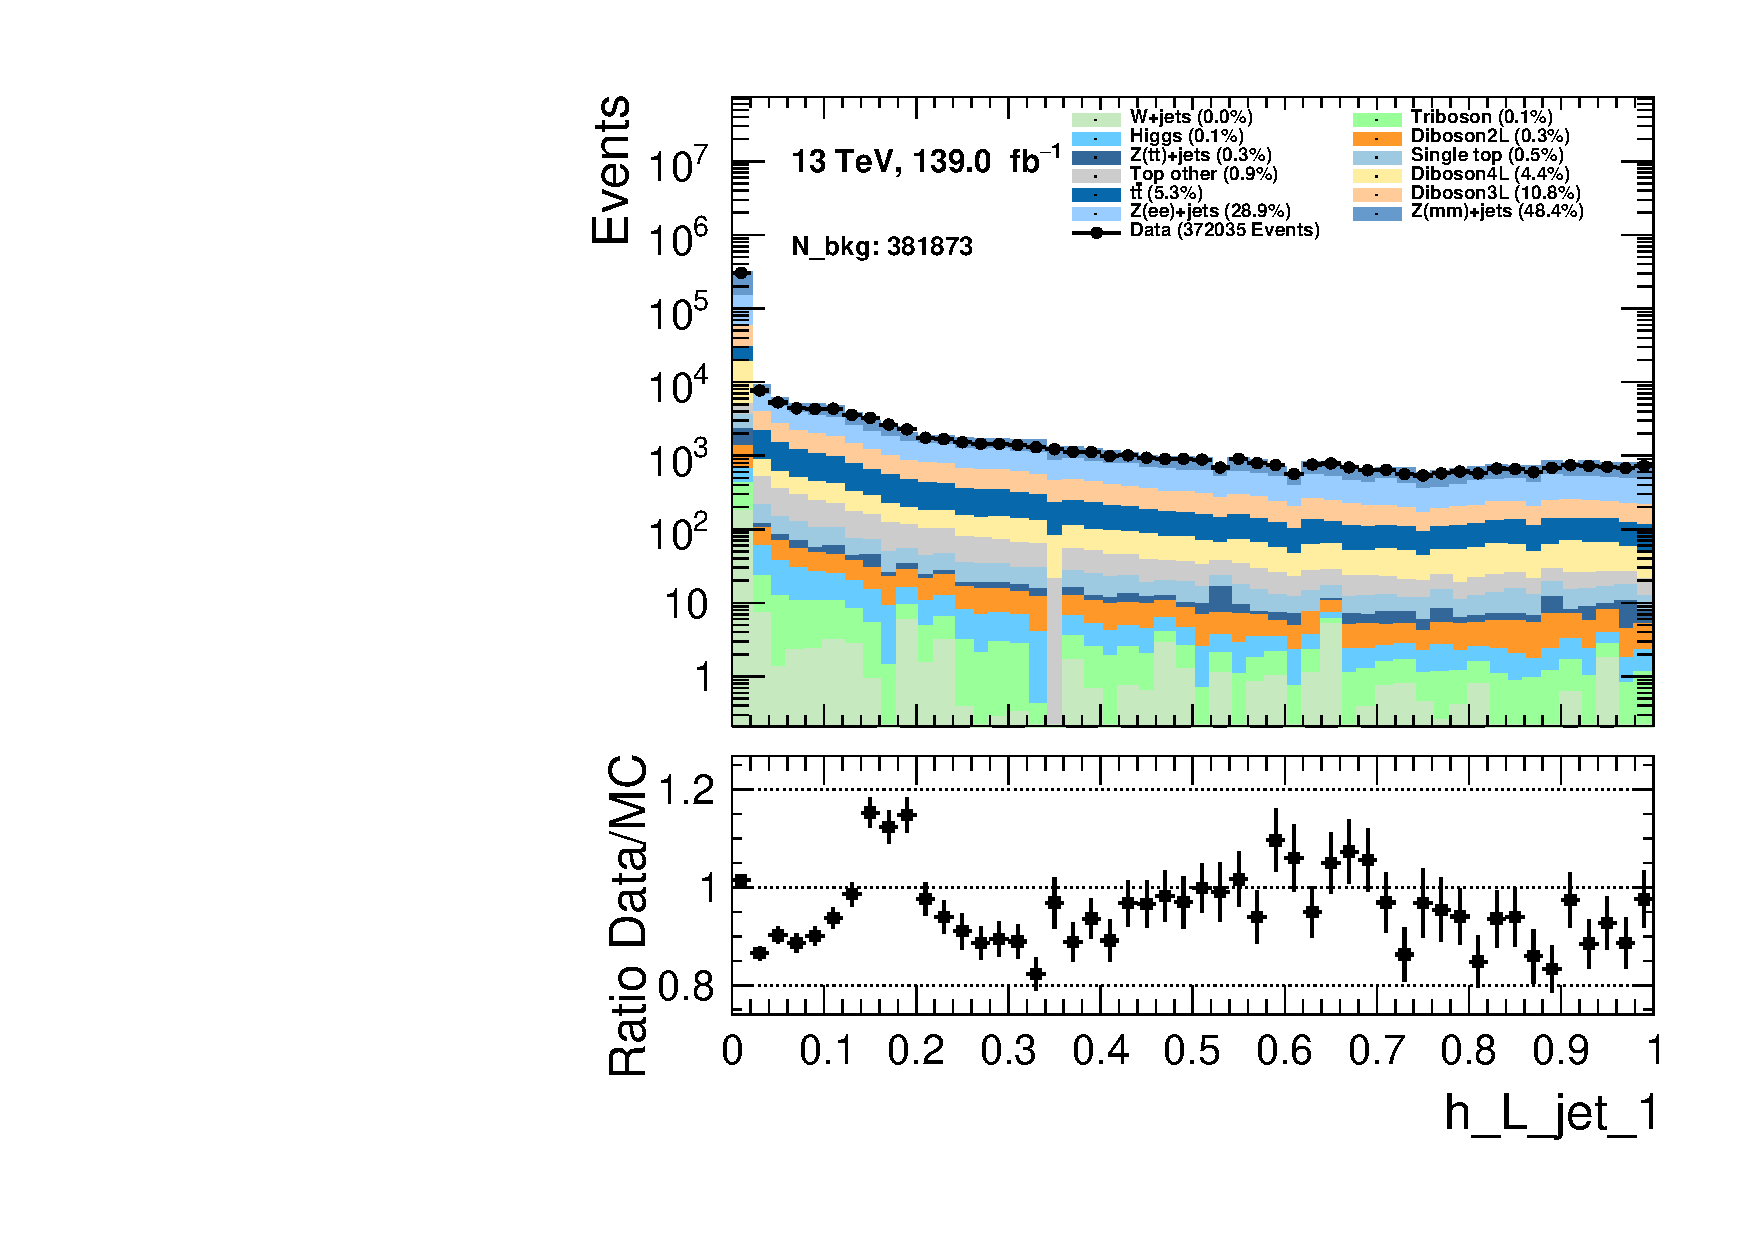
\includegraphics[width=\textwidth]{Figures/MC_Data_comp/h_L_jet_1.pdf}
        \caption{Longitudal component for the second jet.}
        \label{fig:h_L_jet_1}
    \end{subfigure}
    \hfill 
    \begin{subfigure}{.49\textwidth}
        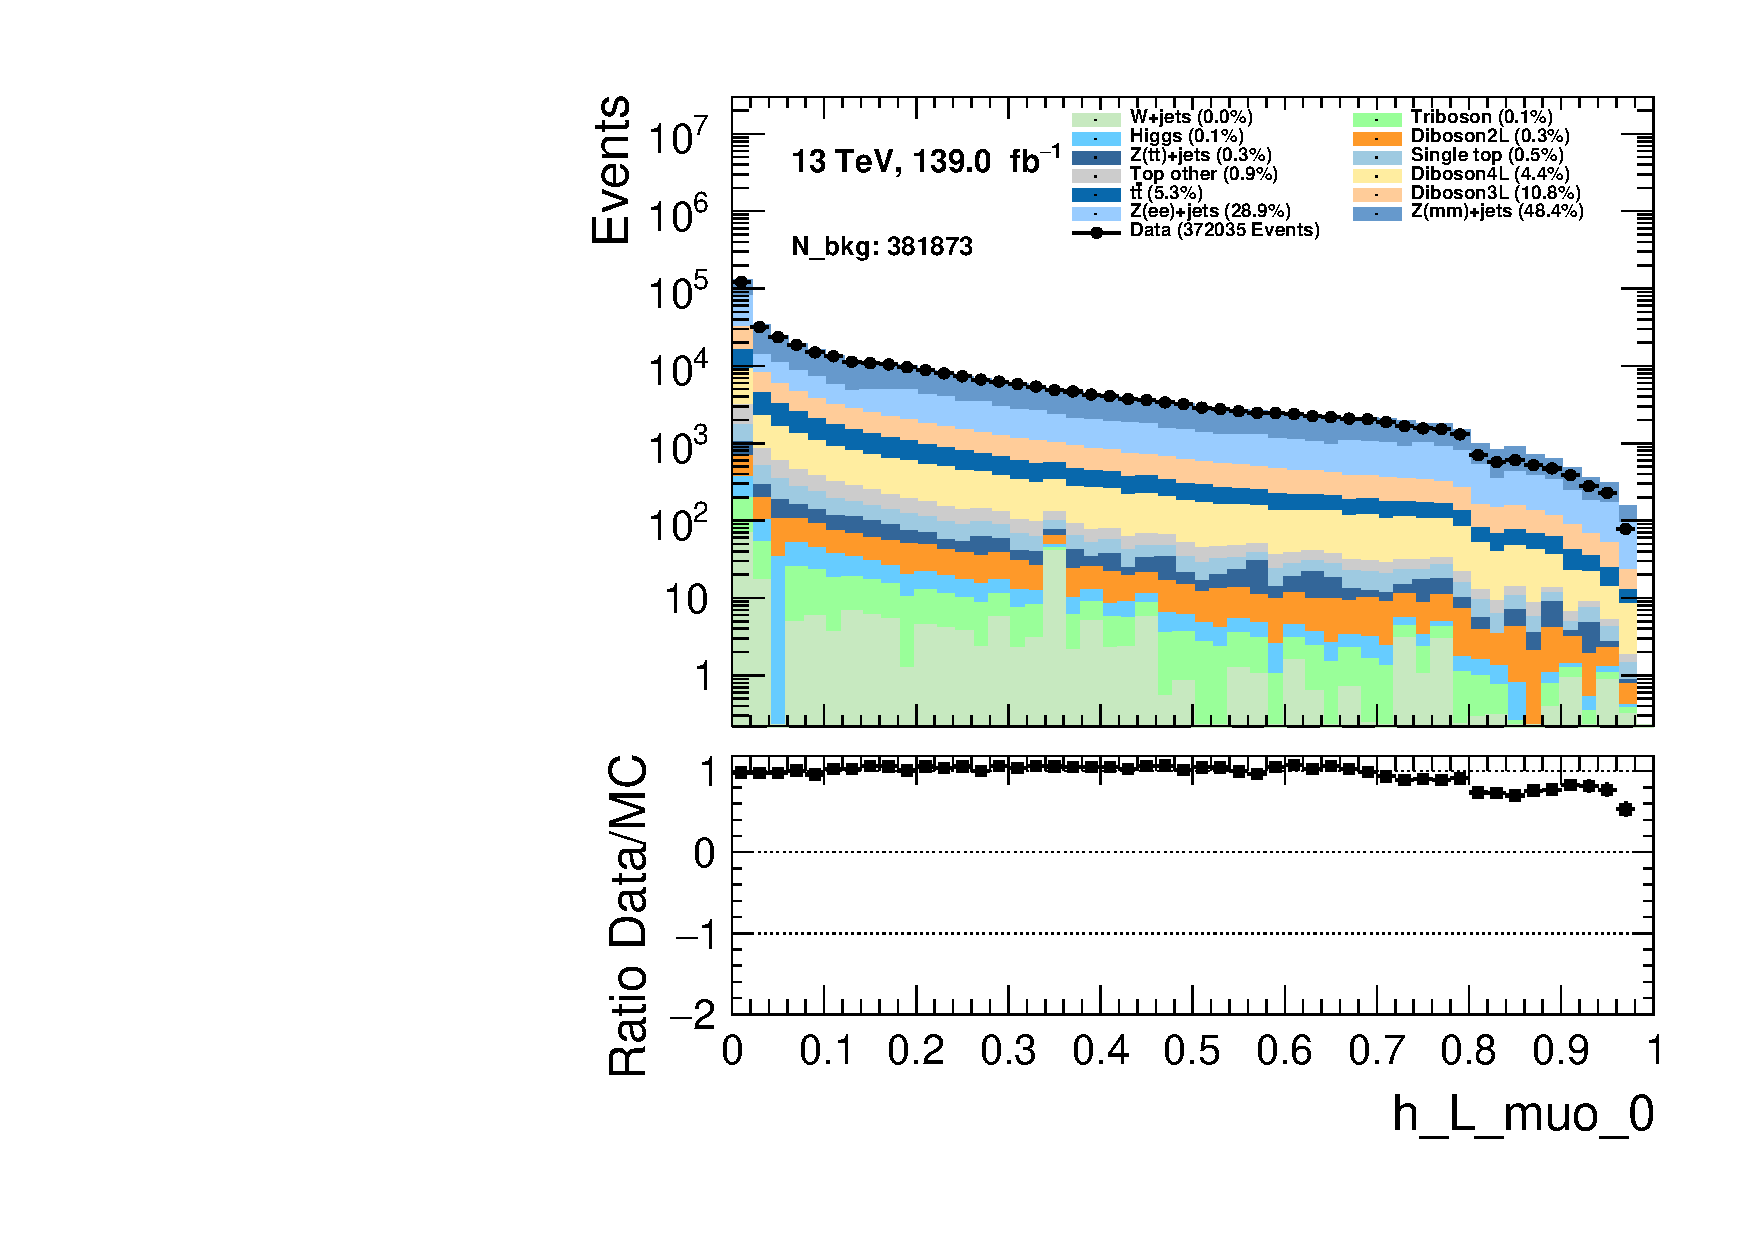
\includegraphics[width=\textwidth]{Figures/MC_Data_comp/h_L_muo_0.pdf}
        \caption{Longitudal component for the first muon.}
        \label{fig:h_L_muo_0}
    \end{subfigure}
    \hfill
    \begin{subfigure}{.49\textwidth}
        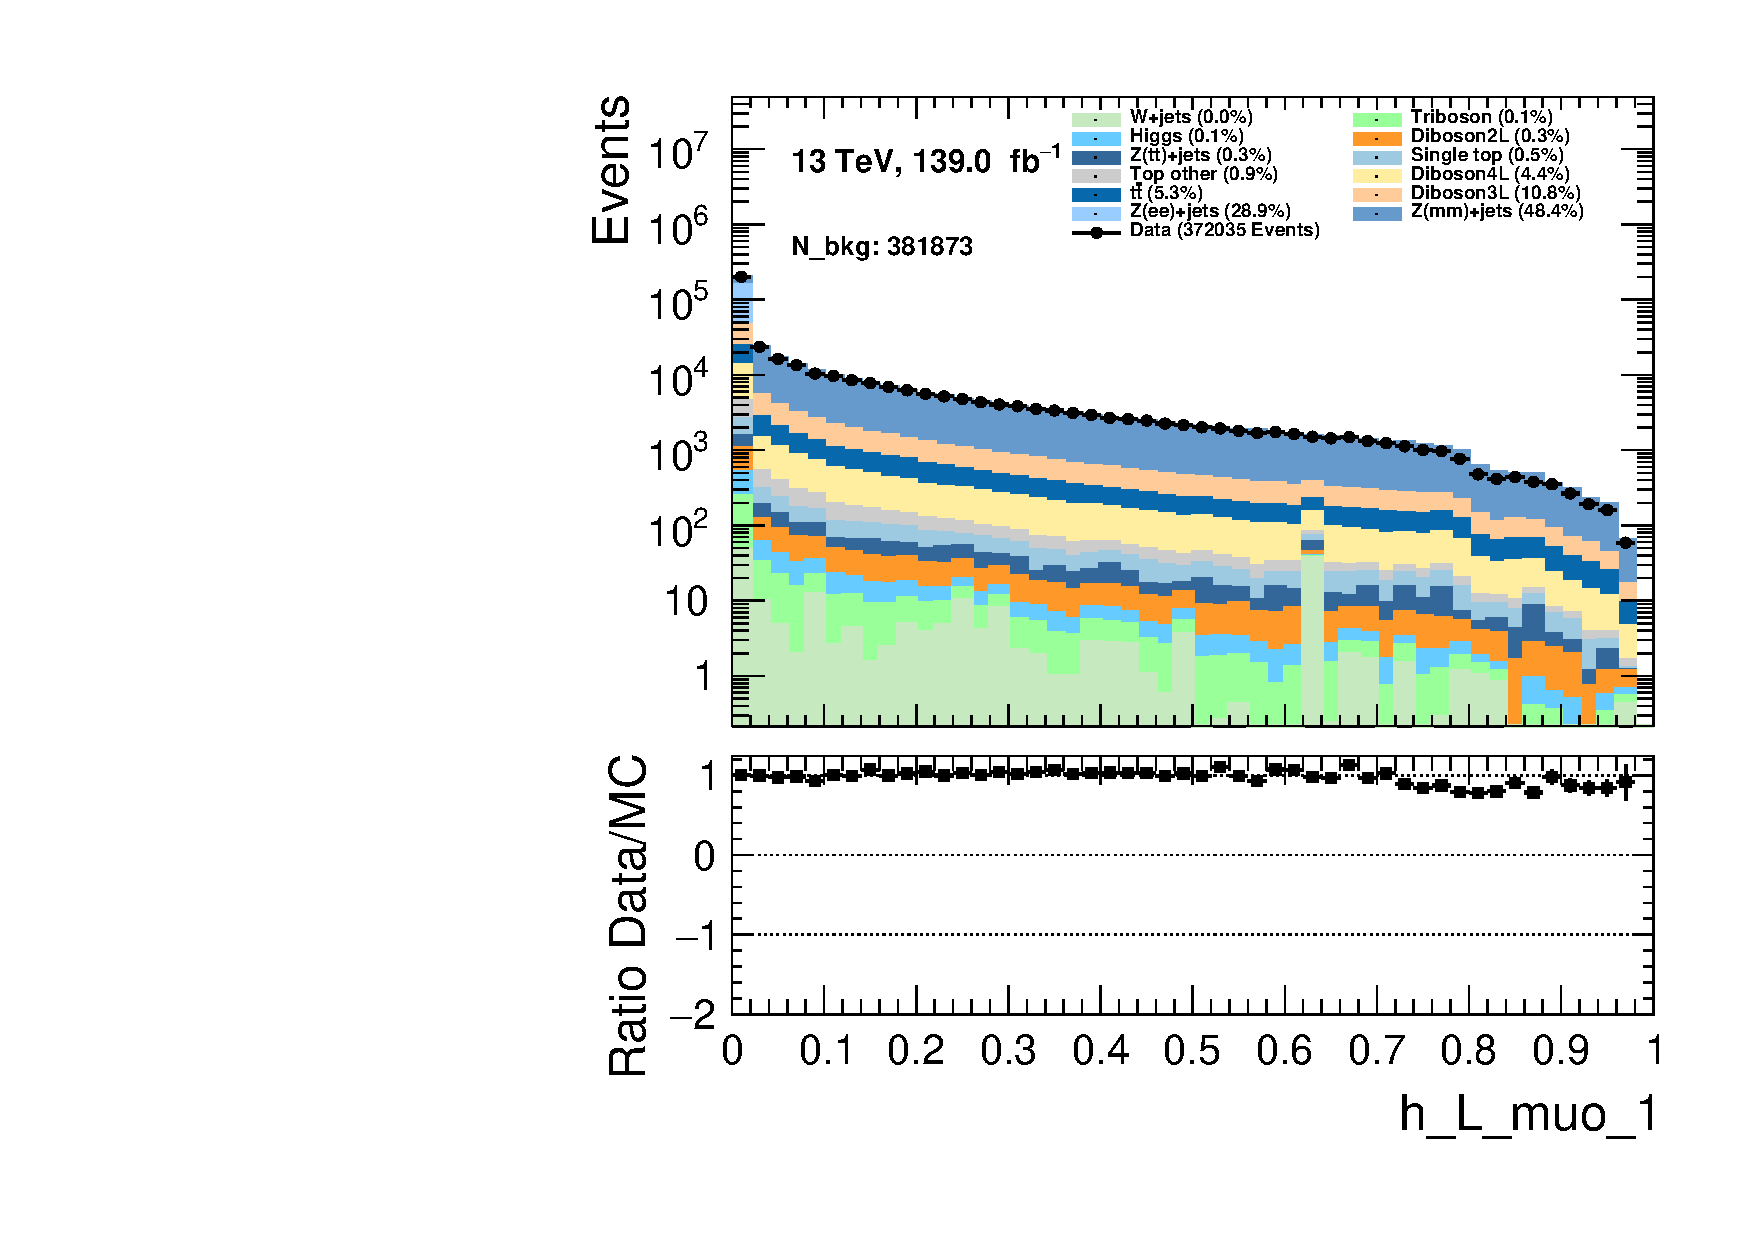
\includegraphics[width=\textwidth]{Figures/MC_Data_comp/h_L_muo_1.pdf}
        \caption{Longitudal component for the second muon.}
        \label{fig:h_L_muo_1}
    \end{subfigure}
    \hfill       
    \caption{Longitudal component for individual particles, here jets and muons.}
    \label{fig:batch7_feats}
\end{figure}

\begin{figure}
    \centering
    \begin{subfigure}{.49\textwidth}
        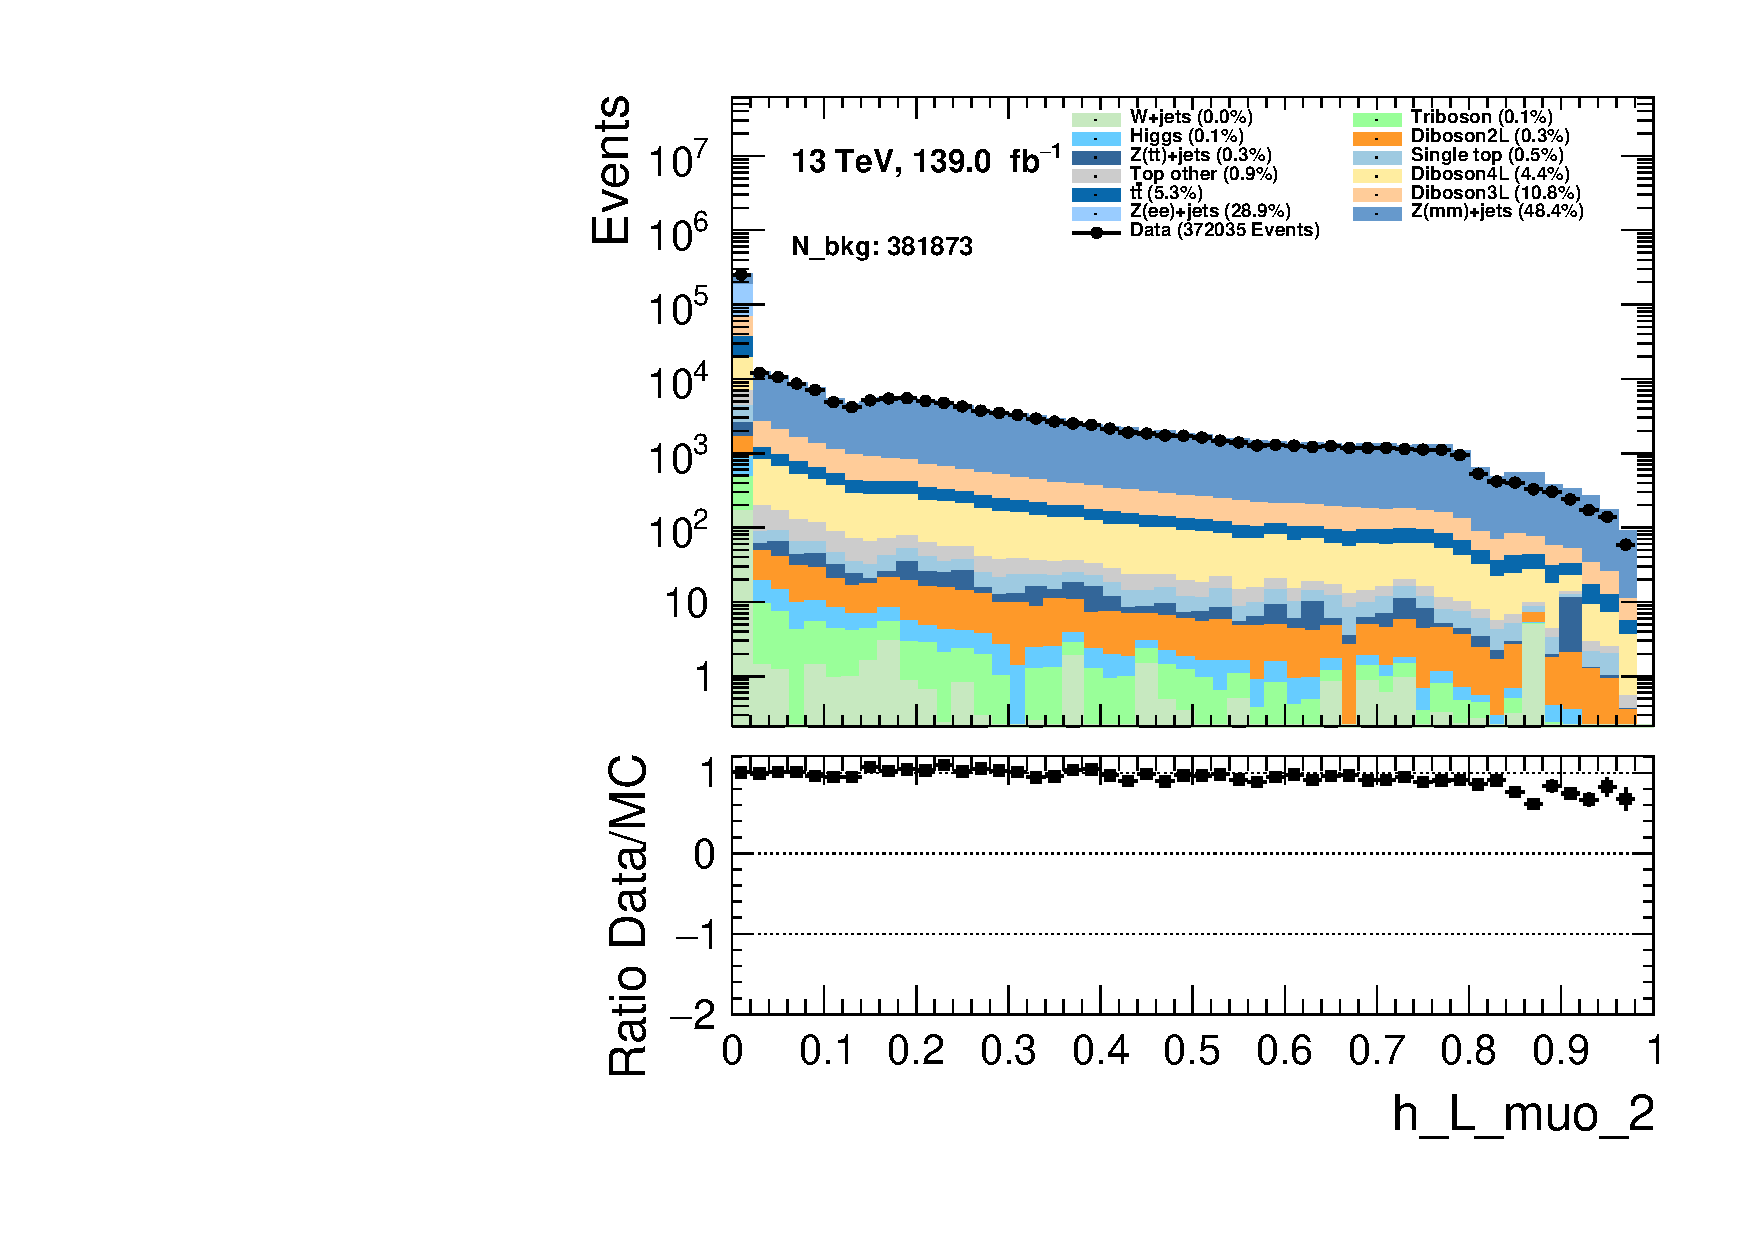
\includegraphics[width=\textwidth]{Figures/MC_Data_comp/h_L_muo_2.pdf}
        \caption{}
        \label{fig:h_L_muo_2}
    \end{subfigure}
    \hfill
    \begin{subfigure}{.49\textwidth}
        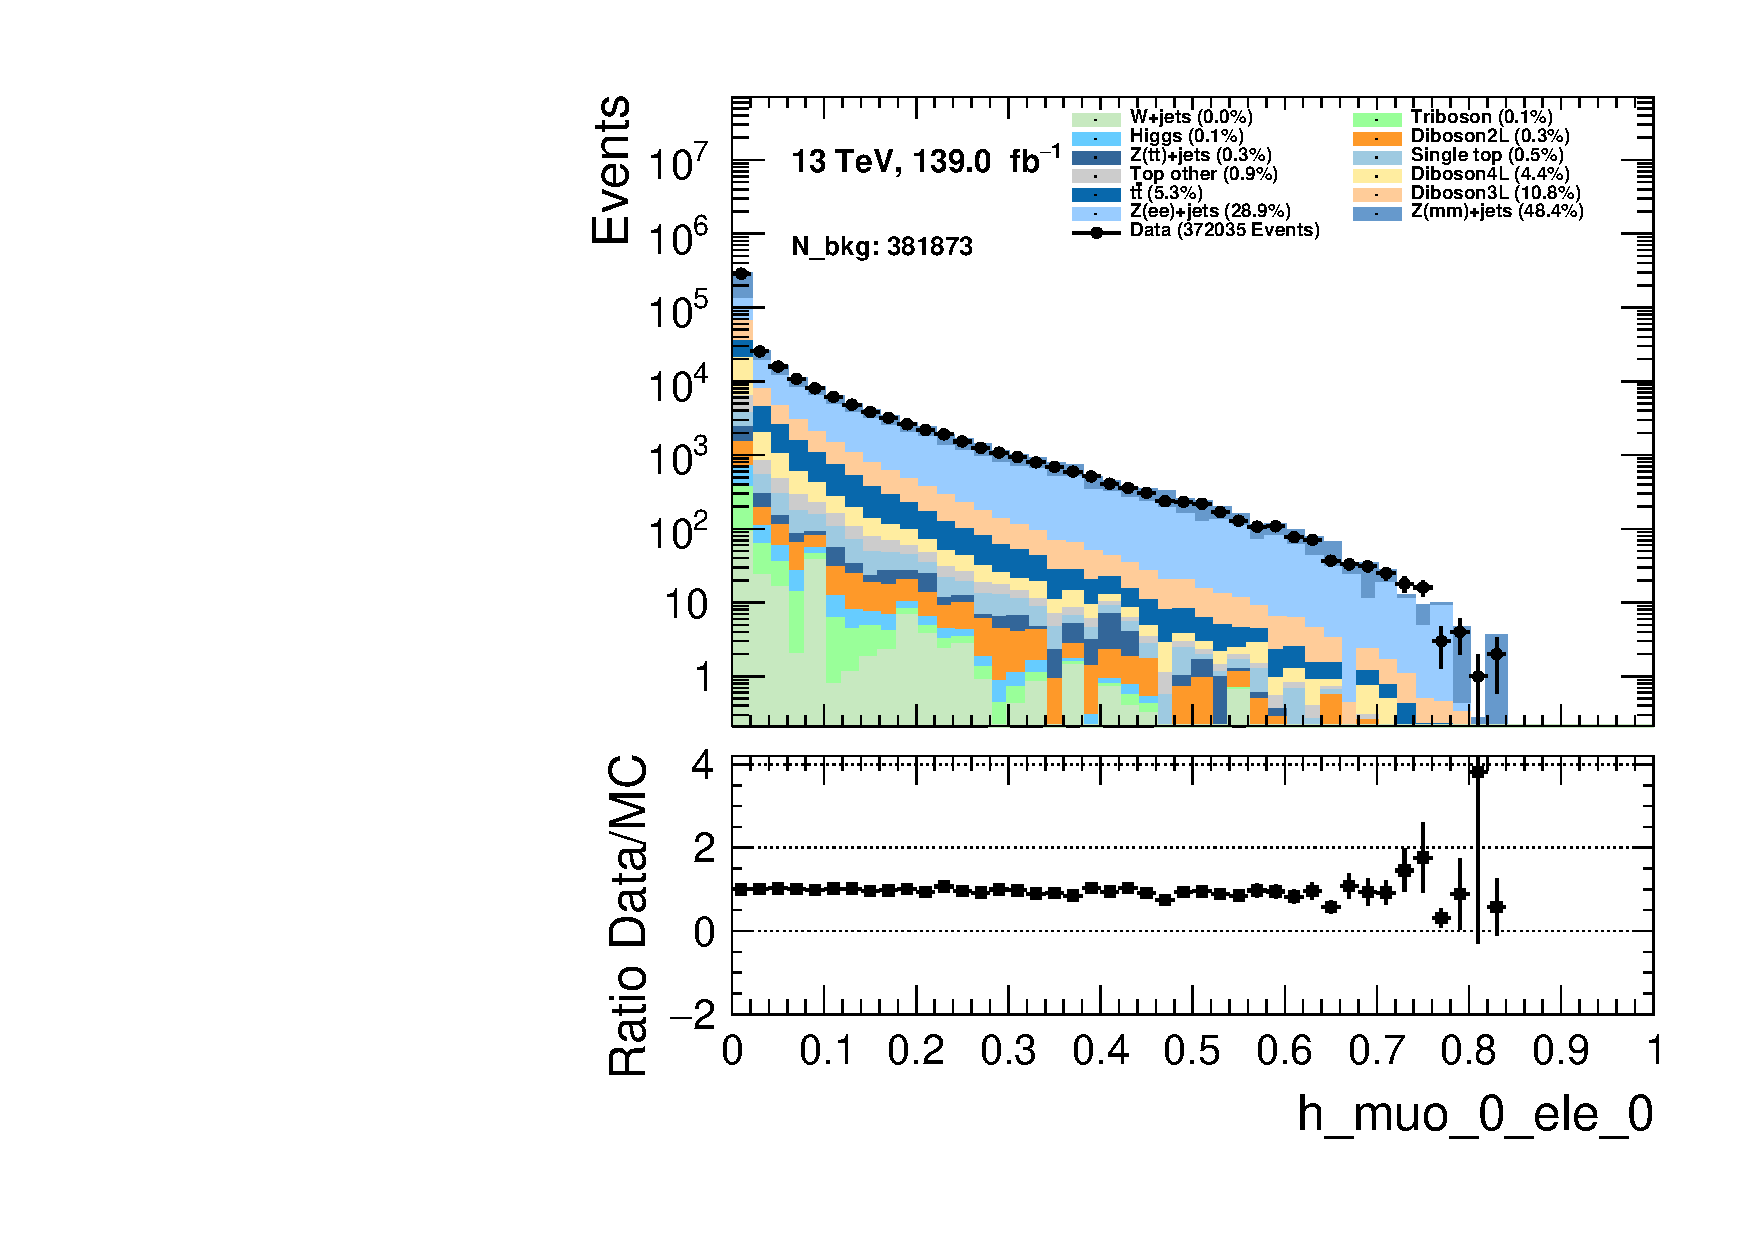
\includegraphics[width=\textwidth]{Figures/MC_Data_comp/h_muo_0_ele_0.pdf}
        \caption{ }
        \label{fig:h_muo_0_ele_0}
    \end{subfigure}
    \hfill 
    \begin{subfigure}{.49\textwidth}
        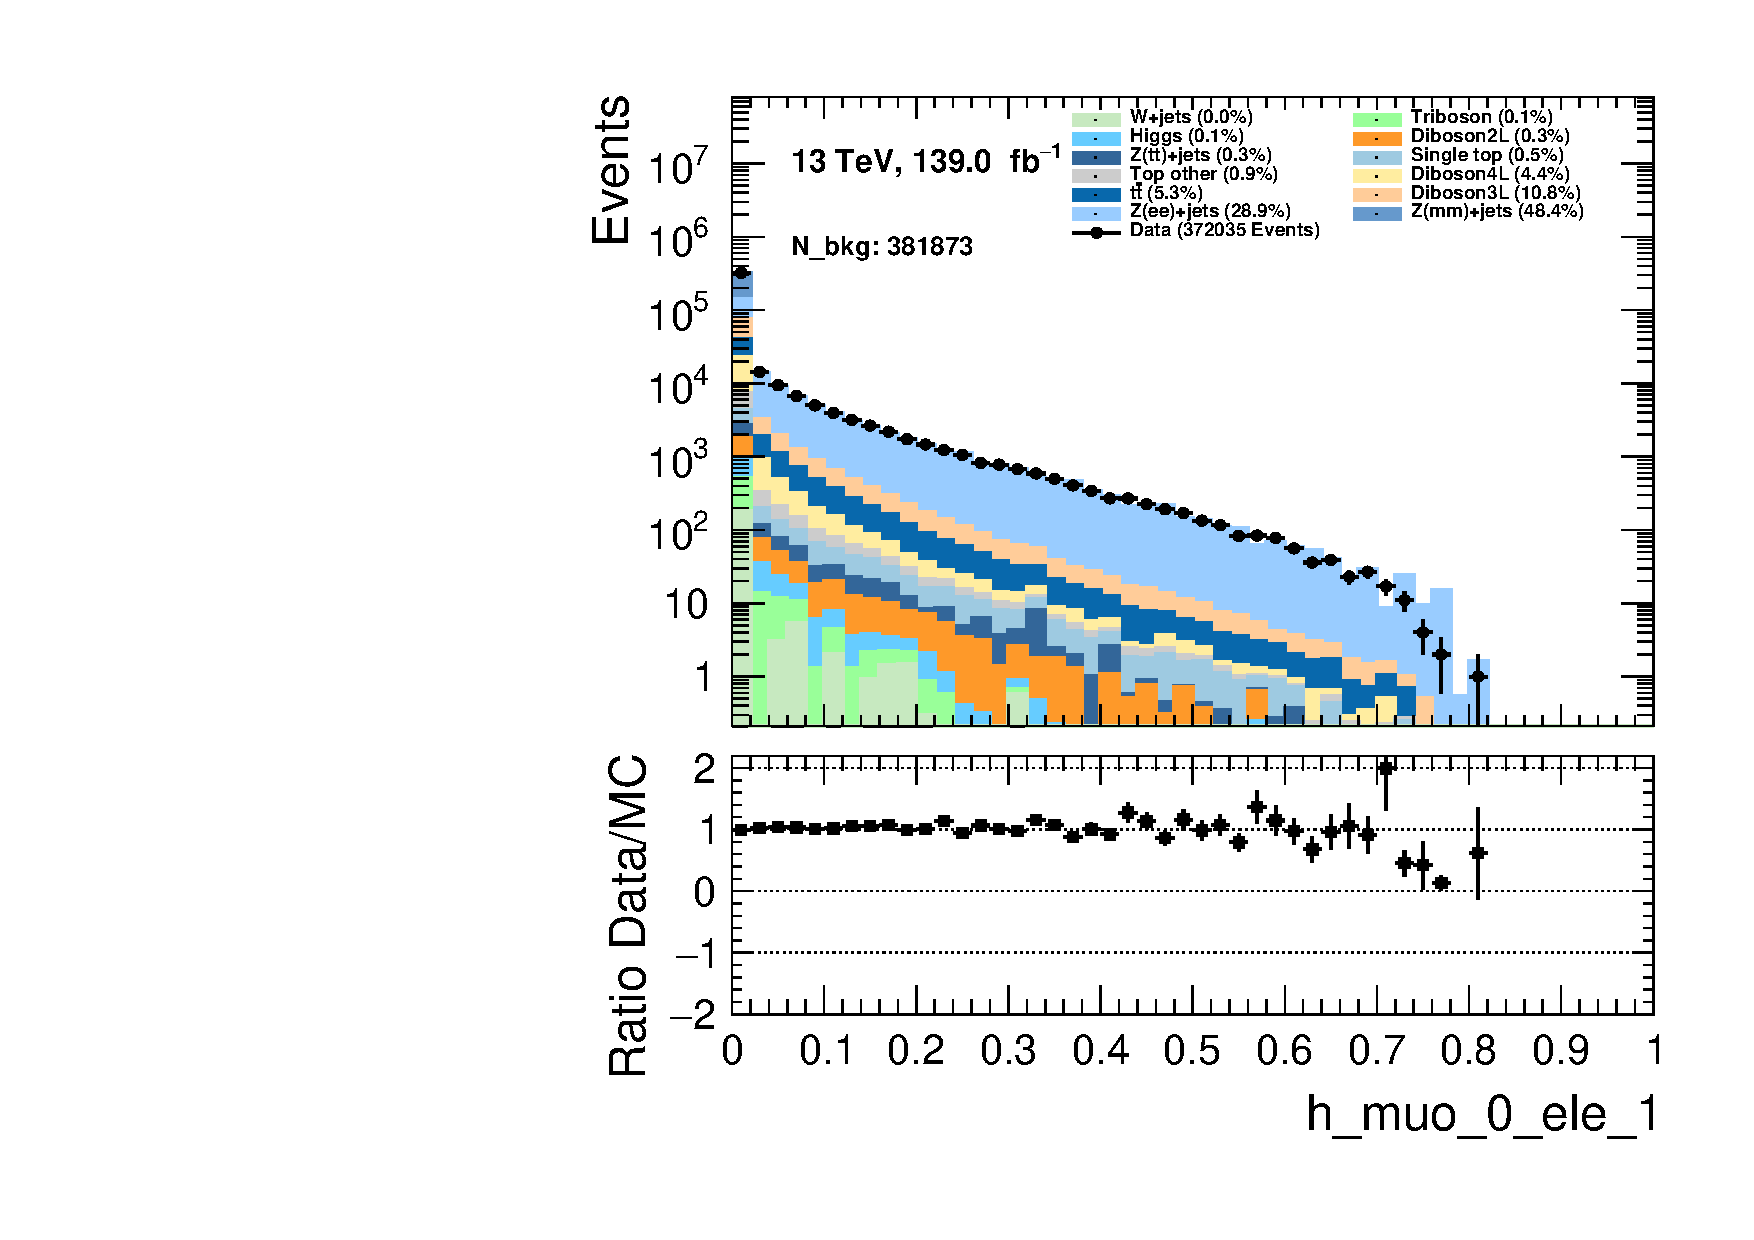
\includegraphics[width=\textwidth]{Figures/MC_Data_comp/h_muo_0_ele_1.pdf}
        \caption{ }
        \label{fig:h_muo_0_ele_1}
    \end{subfigure}
    \hfill
    \begin{subfigure}{.49\textwidth}
        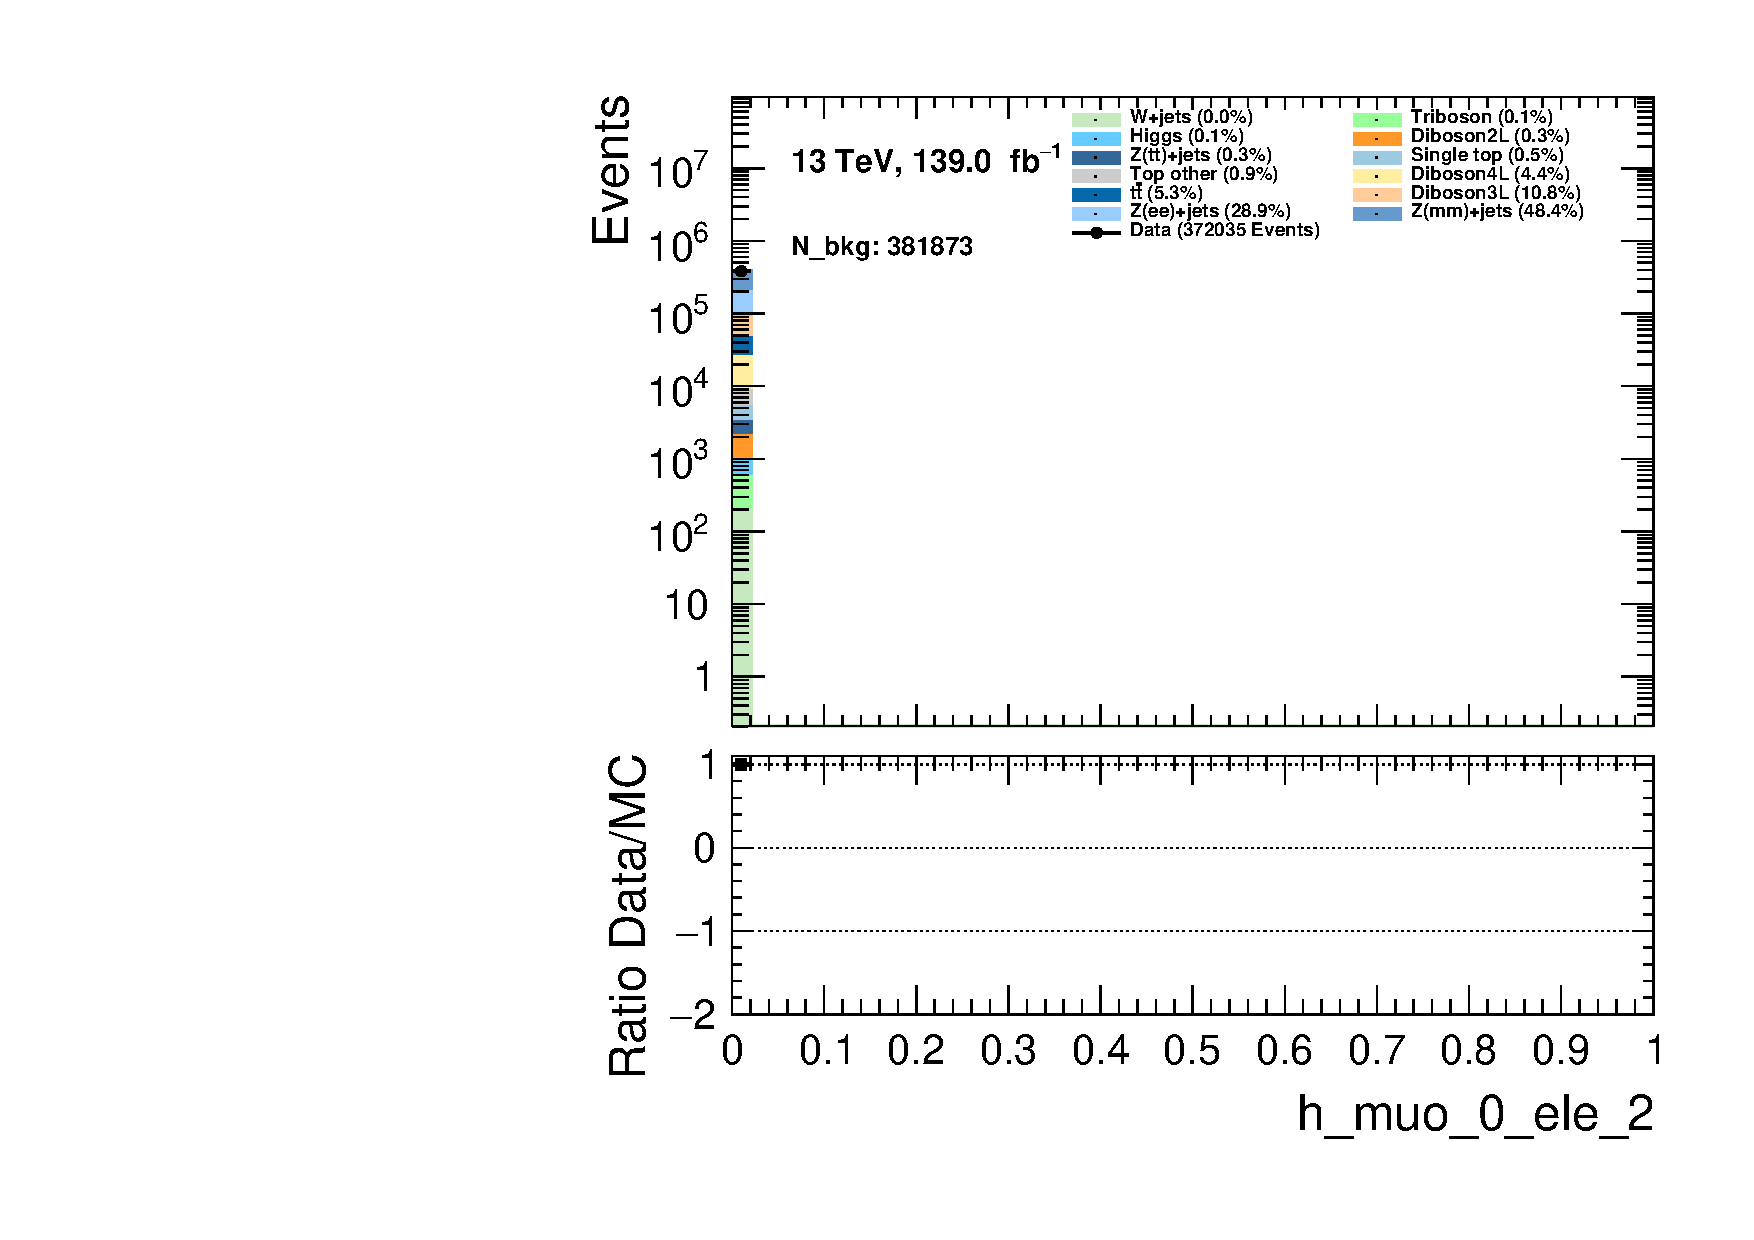
\includegraphics[width=\textwidth]{Figures/MC_Data_comp/h_muo_0_ele_2.pdf}
        \caption{ }
        \label{fig:h_muo_0_ele_2}
    \end{subfigure}
    \hfill       
    \caption{}
    \label{fig:t}
\end{figure}


\begin{figure}
    \centering
    \begin{subfigure}{.49\textwidth}
        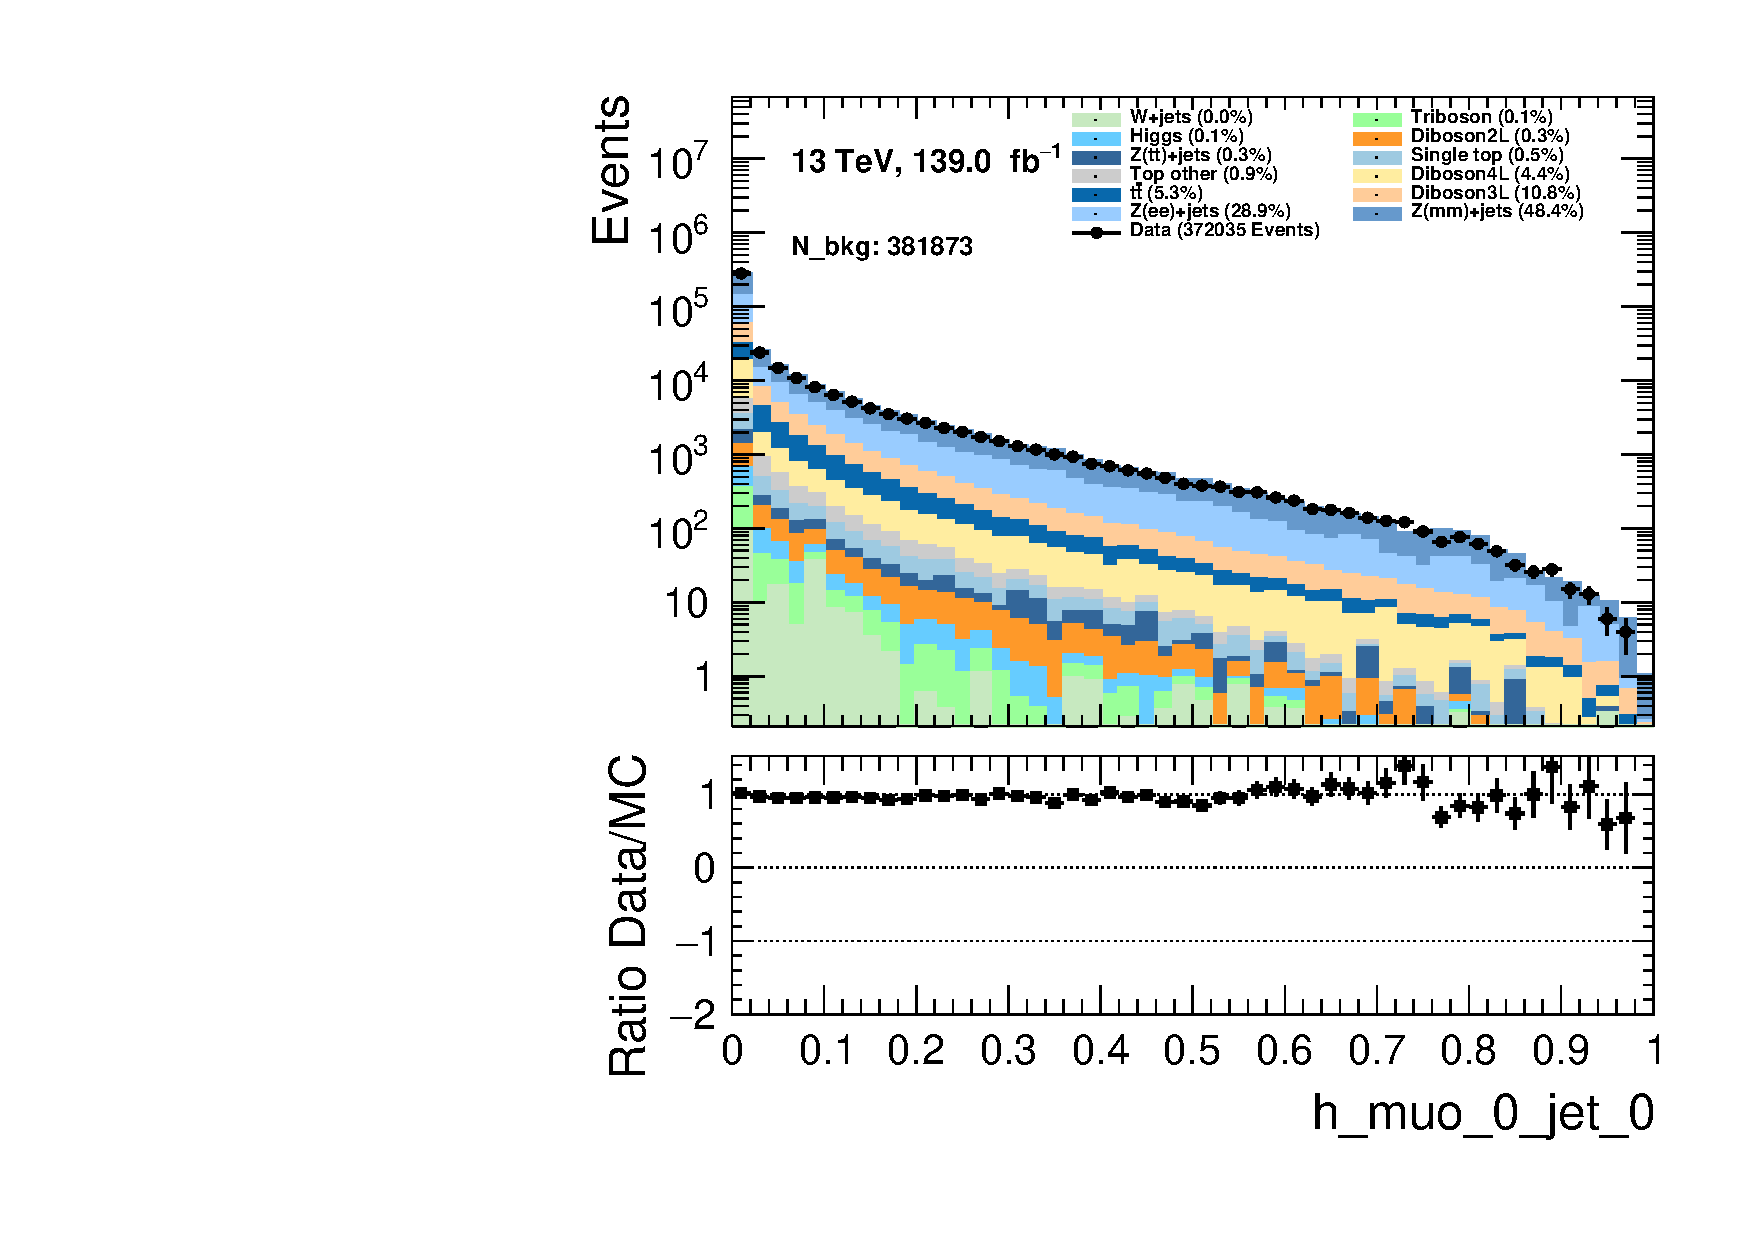
\includegraphics[width=\textwidth]{Figures/MC_Data_comp/h_muo_0_jet_0.pdf}
        \caption{}
        \label{fig:et}
    \end{subfigure}
    \hfill
    \begin{subfigure}{.49\textwidth}
        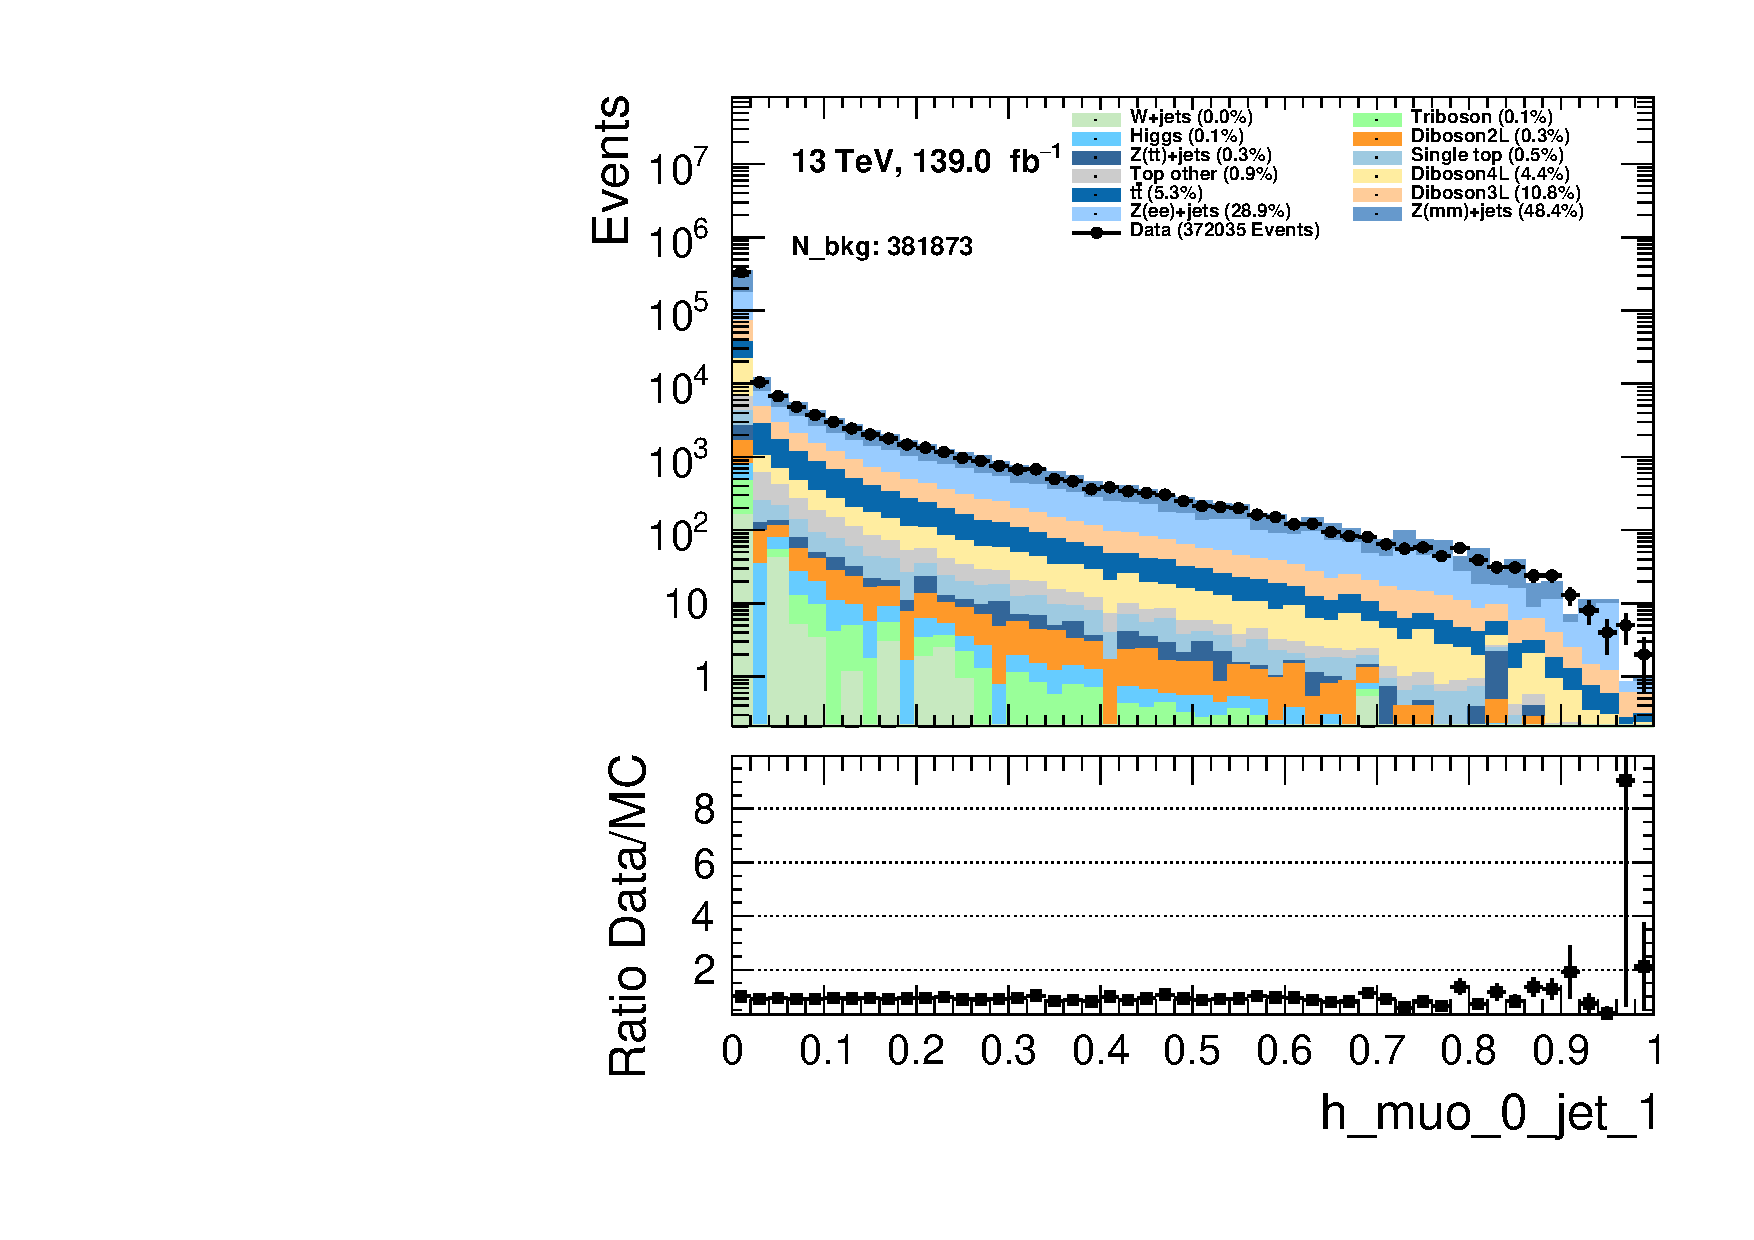
\includegraphics[width=\textwidth]{Figures/MC_Data_comp/h_muo_0_jet_1.pdf}
        \caption{ }
        \label{fig:flcp}
    \end{subfigure}
    \hfill 
    \begin{subfigure}{.49\textwidth}
        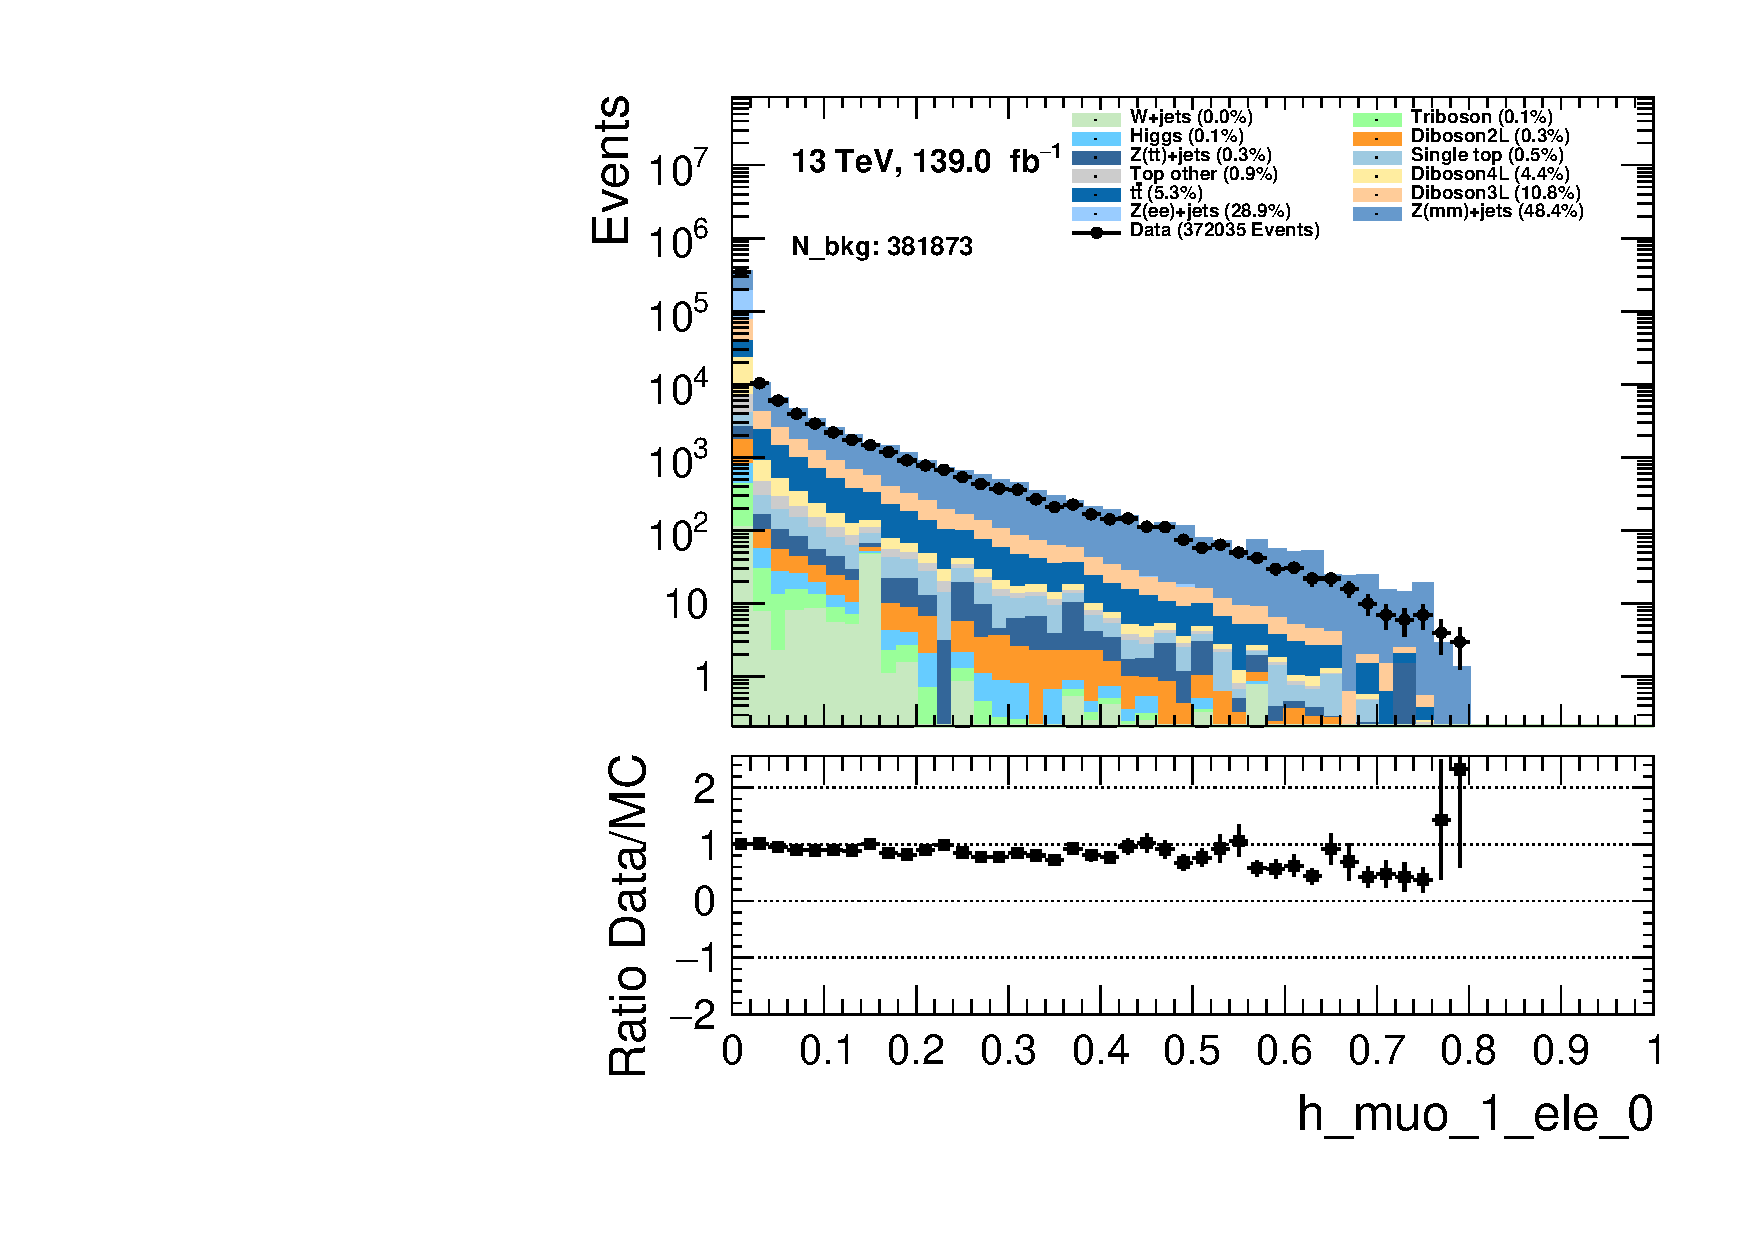
\includegraphics[width=\textwidth]{Figures/MC_Data_comp/h_muo_1_ele_0.pdf}
        \caption{ }
        \label{fig:fep}
    \end{subfigure}
    \hfill
    \begin{subfigure}{.49\textwidth}
        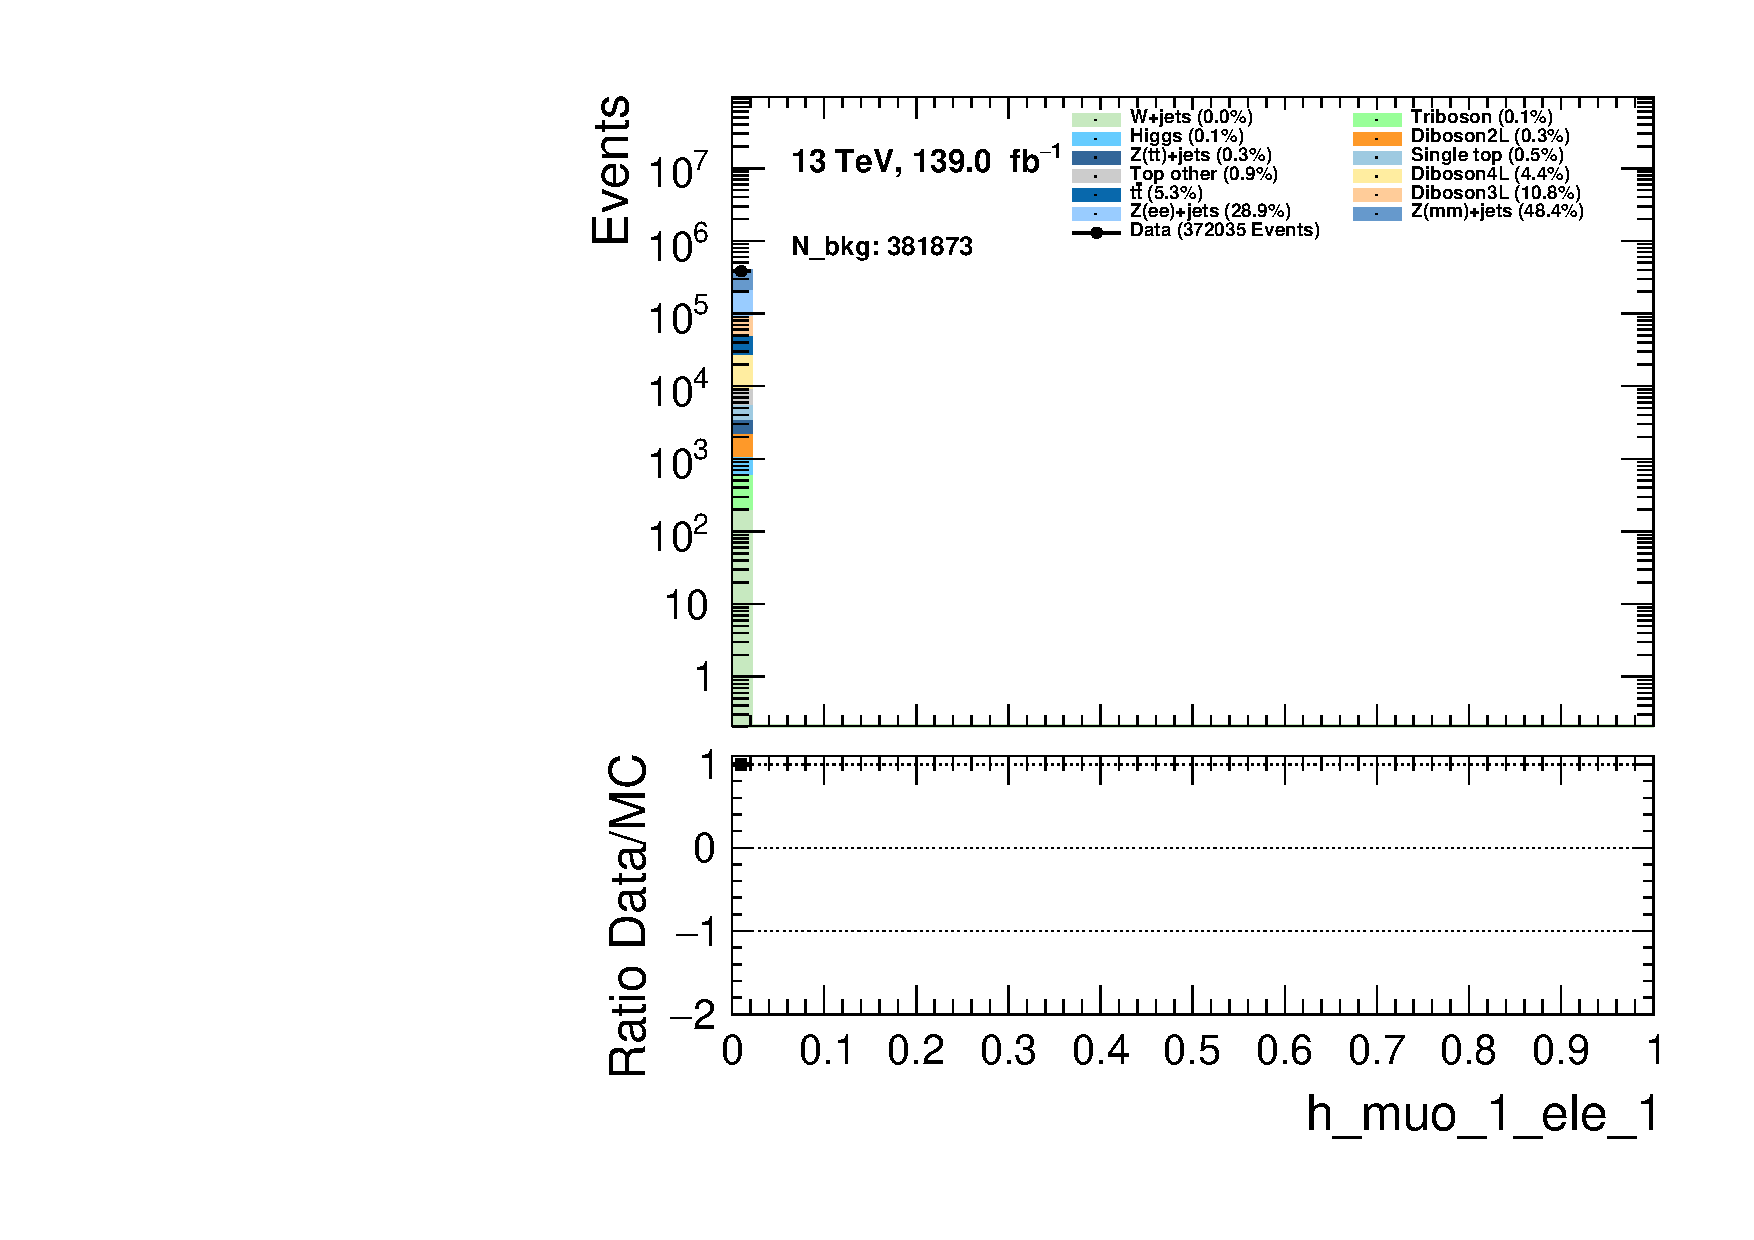
\includegraphics[width=\textwidth]{Figures/MC_Data_comp/h_muo_1_ele_1.pdf}
        \caption{ }
        \label{fig:fe}
    \end{subfigure}
    \hfill       
    \caption{}
    \label{fig:t}
\end{figure}

\begin{figure}
    \centering
    \begin{subfigure}{.49\textwidth}
        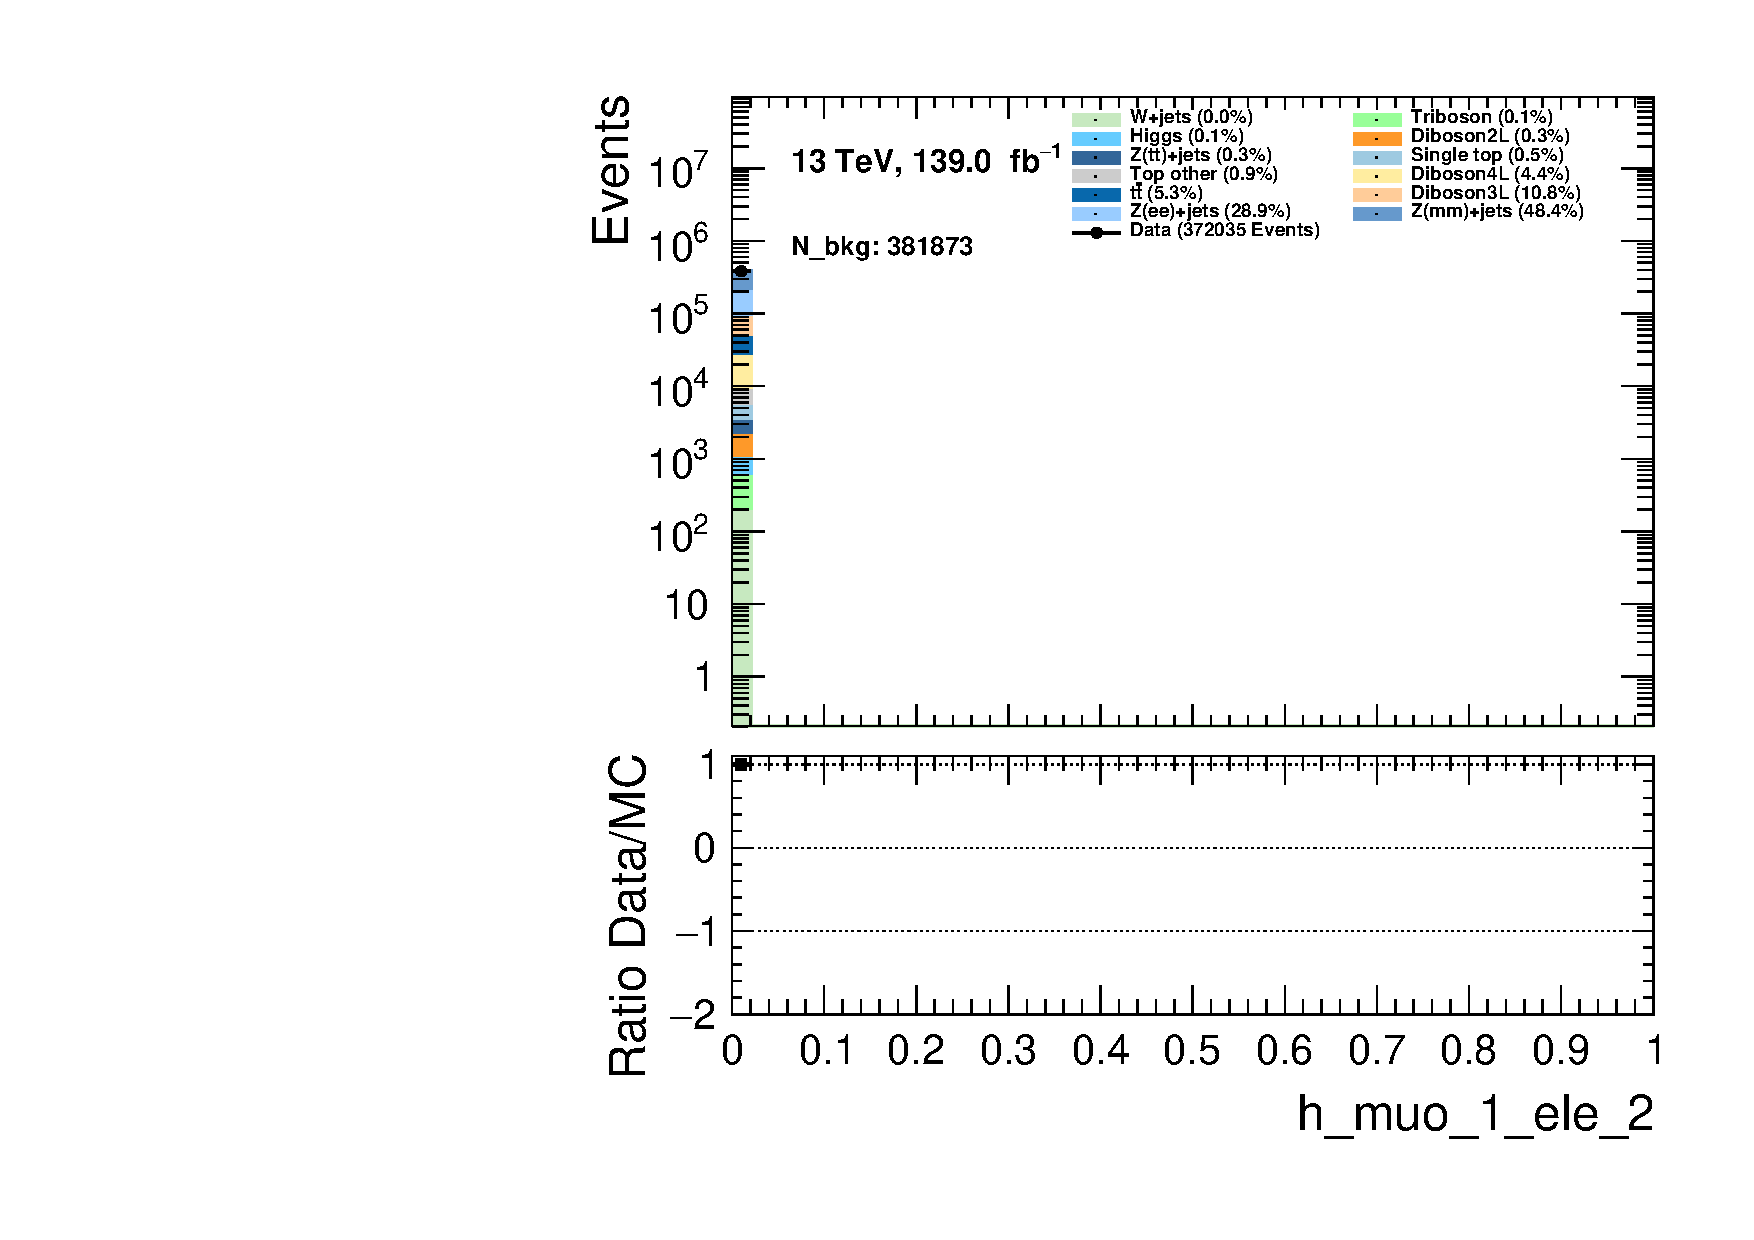
\includegraphics[width=\textwidth]{Figures/MC_Data_comp/h_muo_1_ele_2.pdf}
        \caption{}
        \label{fig:et}
    \end{subfigure}
    \hfill
    \begin{subfigure}{.49\textwidth}
        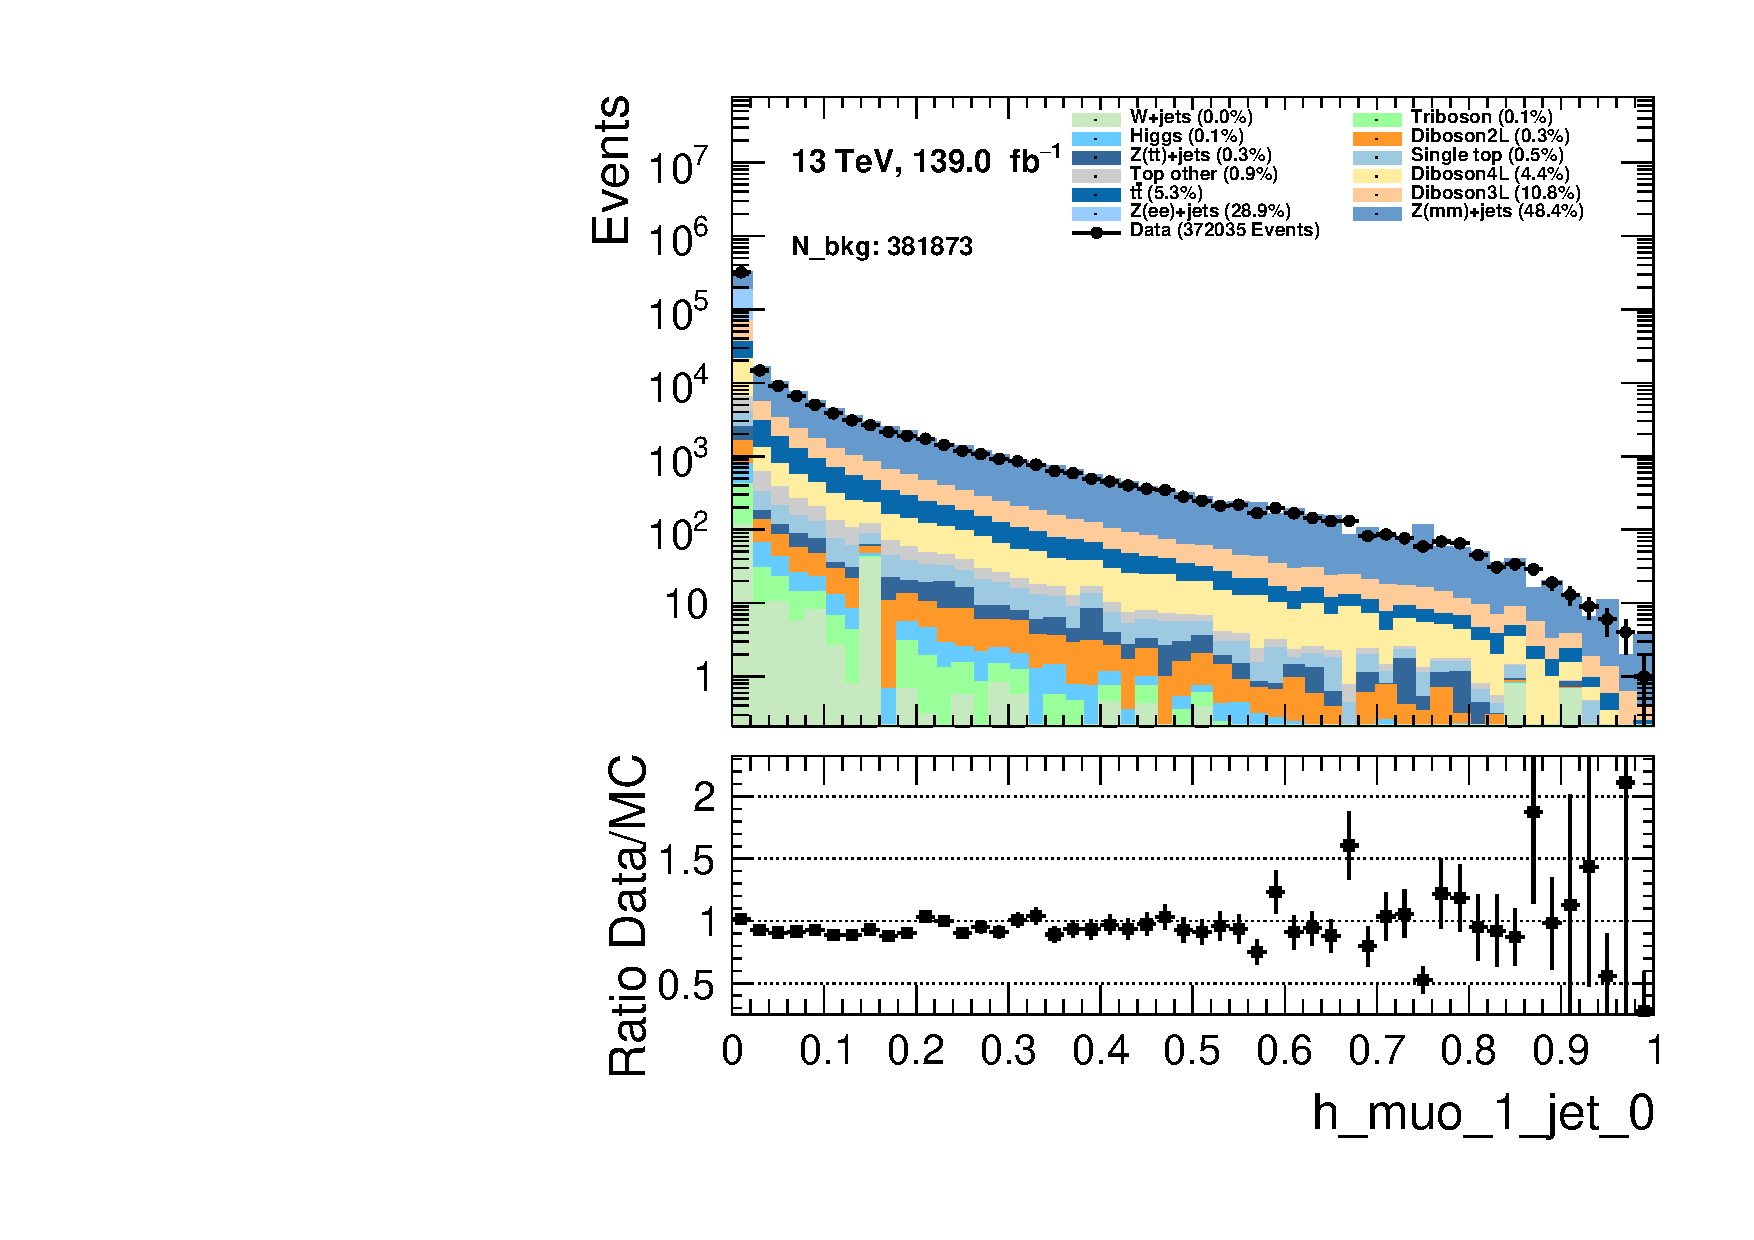
\includegraphics[width=\textwidth]{Figures/MC_Data_comp/h_muo_1_jet_0.pdf}
        \caption{ }
        \label{fig:flcp}
    \end{subfigure}
    \hfill 
    \begin{subfigure}{.49\textwidth}
        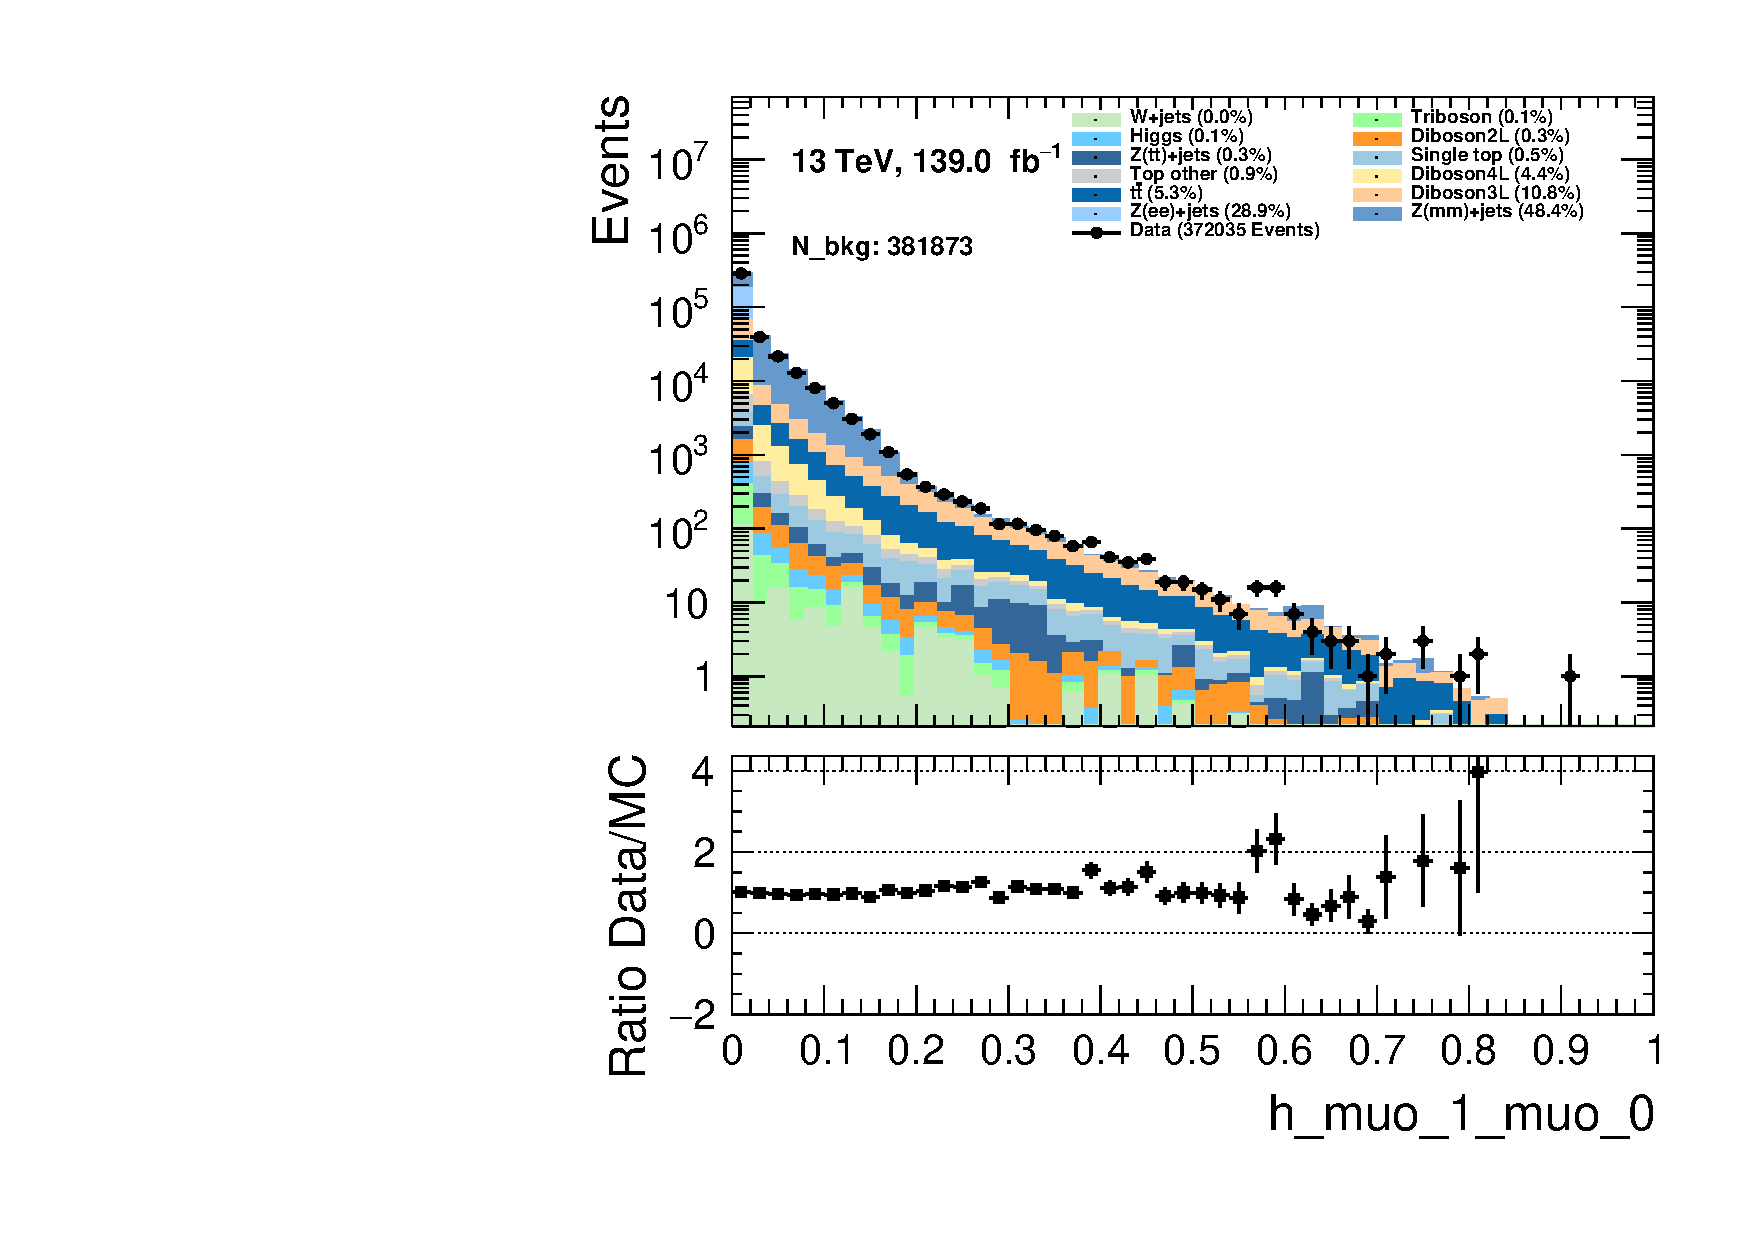
\includegraphics[width=\textwidth]{Figures/MC_Data_comp/h_muo_1_muo_0.pdf}
        \caption{ }
        \label{fig:fep}
    \end{subfigure}
    \hfill
    \begin{subfigure}{.49\textwidth}
        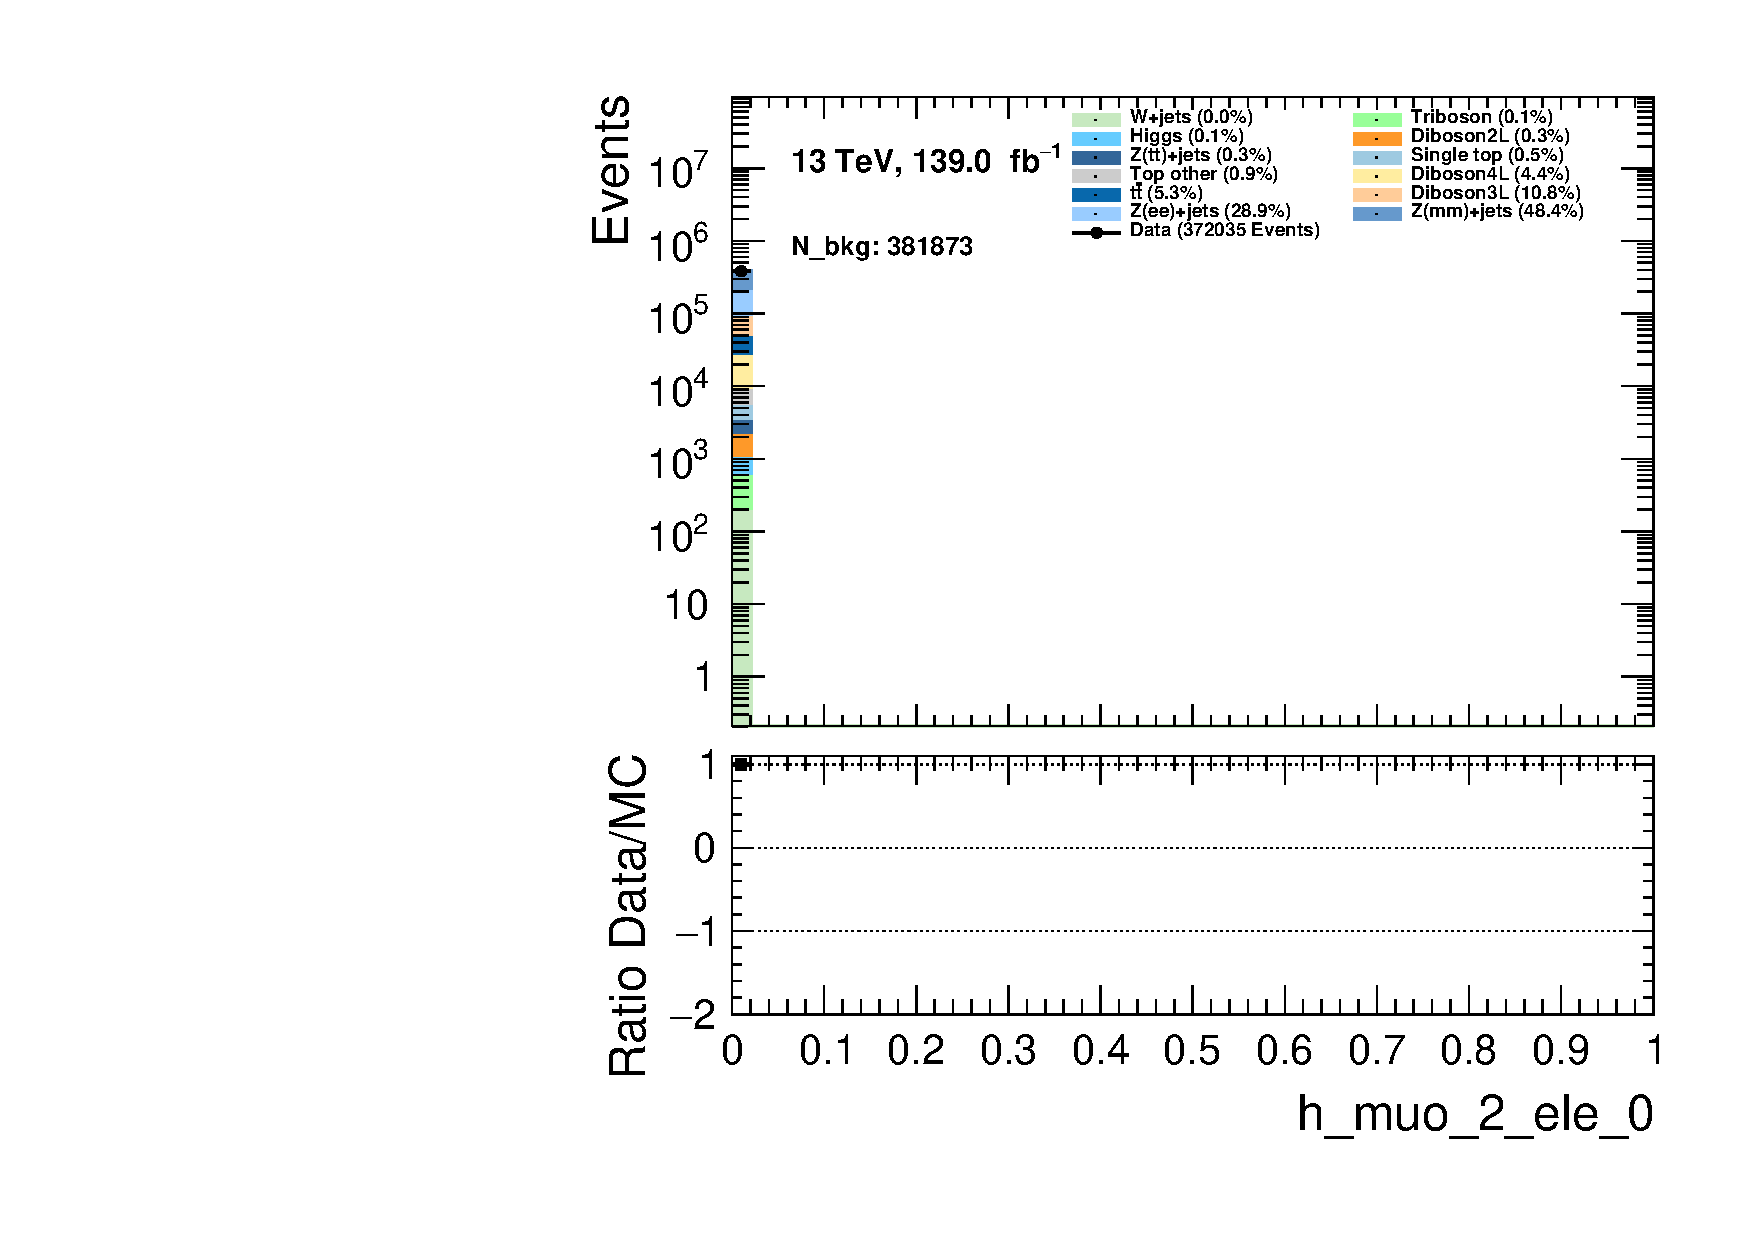
\includegraphics[width=\textwidth]{Figures/MC_Data_comp/h_muo_2_ele_0.pdf}
        \caption{ }
        \label{fig:fe}
    \end{subfigure}
    \hfill       
    \caption{}
    \label{fig:t}
\end{figure}

\begin{figure}
    \centering
    \begin{subfigure}{.49\textwidth}
        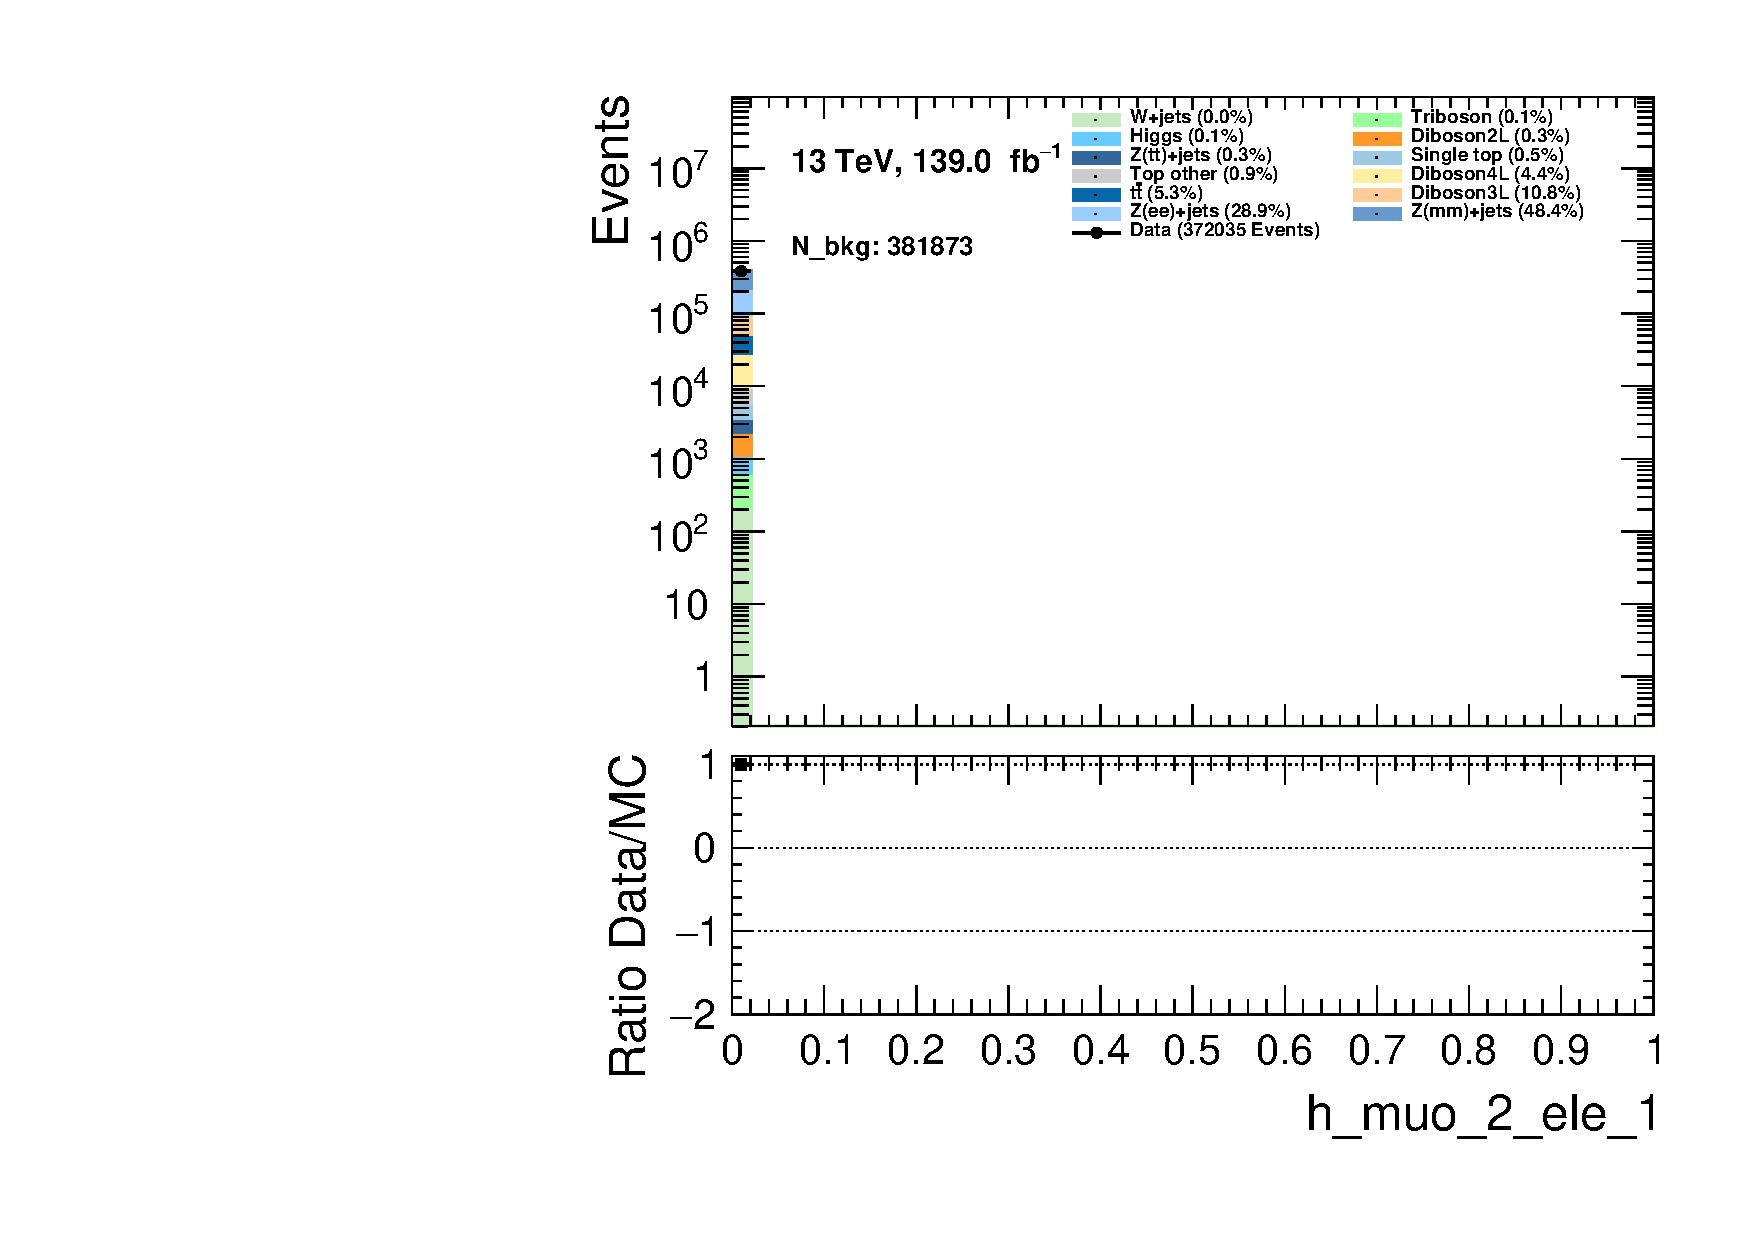
\includegraphics[width=\textwidth]{Figures/MC_Data_comp/h_muo_2_ele_1.pdf}
        \caption{}
        \label{fig:et}
    \end{subfigure}
    \hfill
    \begin{subfigure}{.49\textwidth}
        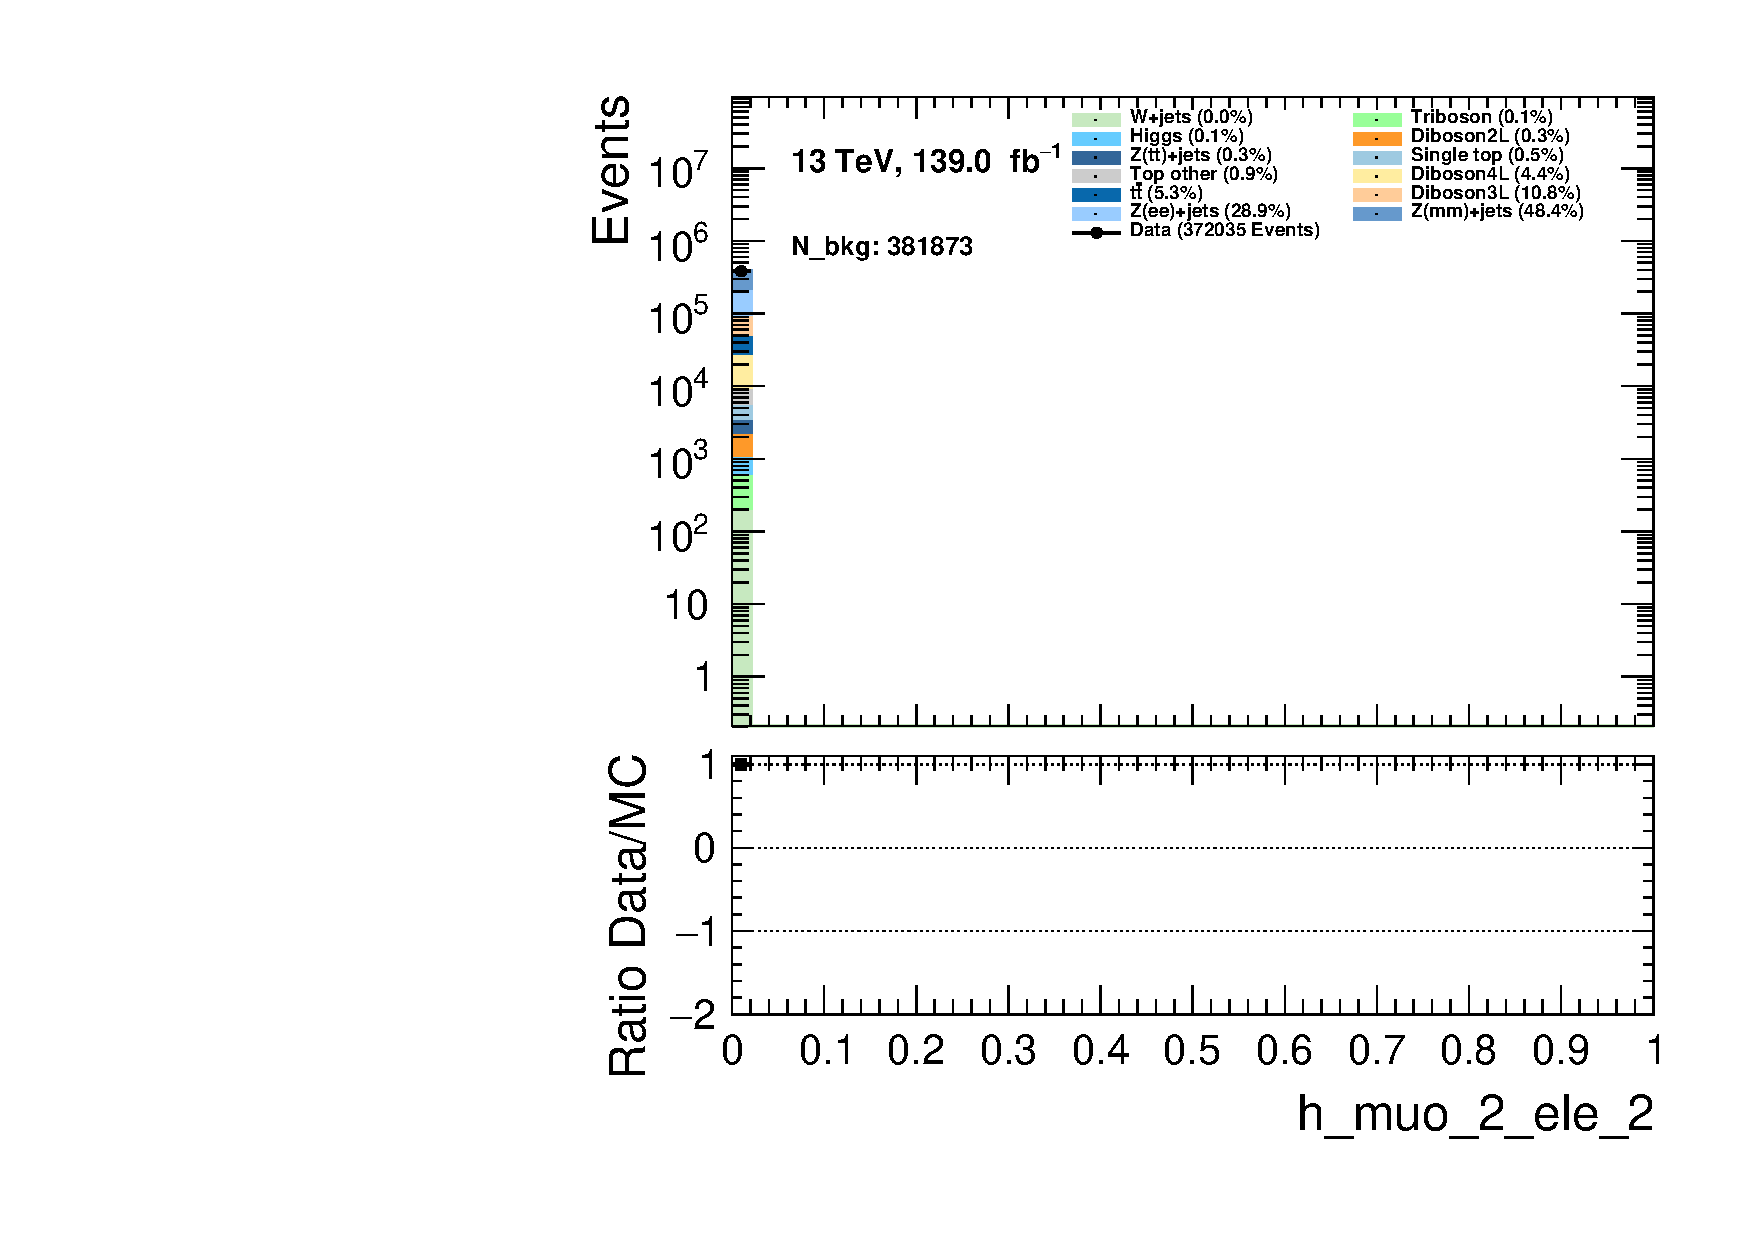
\includegraphics[width=\textwidth]{Figures/MC_Data_comp/h_muo_2_ele_2.pdf}
        \caption{ }
        \label{fig:flcp}
    \end{subfigure}
    \hfill 
    \begin{subfigure}{.49\textwidth}
        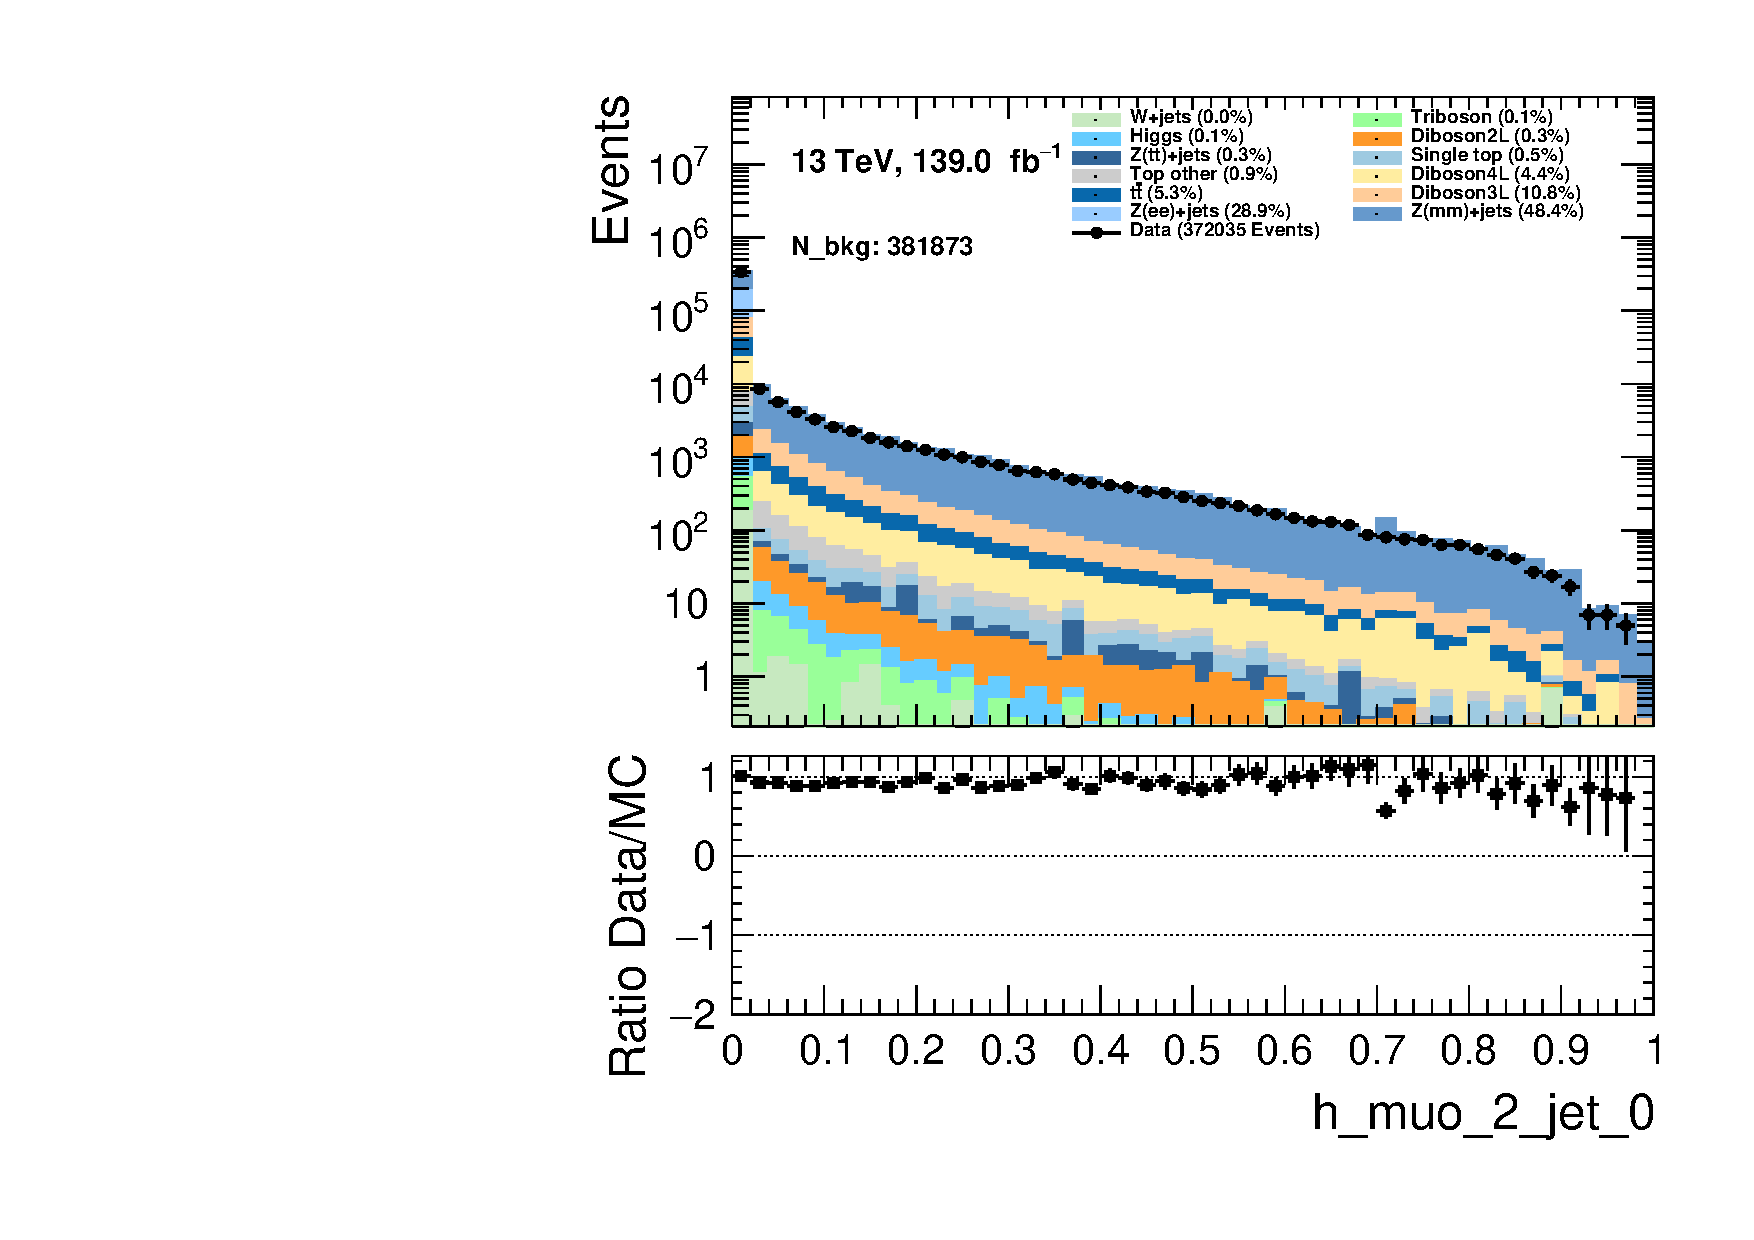
\includegraphics[width=\textwidth]{Figures/MC_Data_comp/h_muo_2_jet_0.pdf}
        \caption{ }
        \label{fig:fep}
    \end{subfigure}
    \hfill
    \begin{subfigure}{.49\textwidth}
        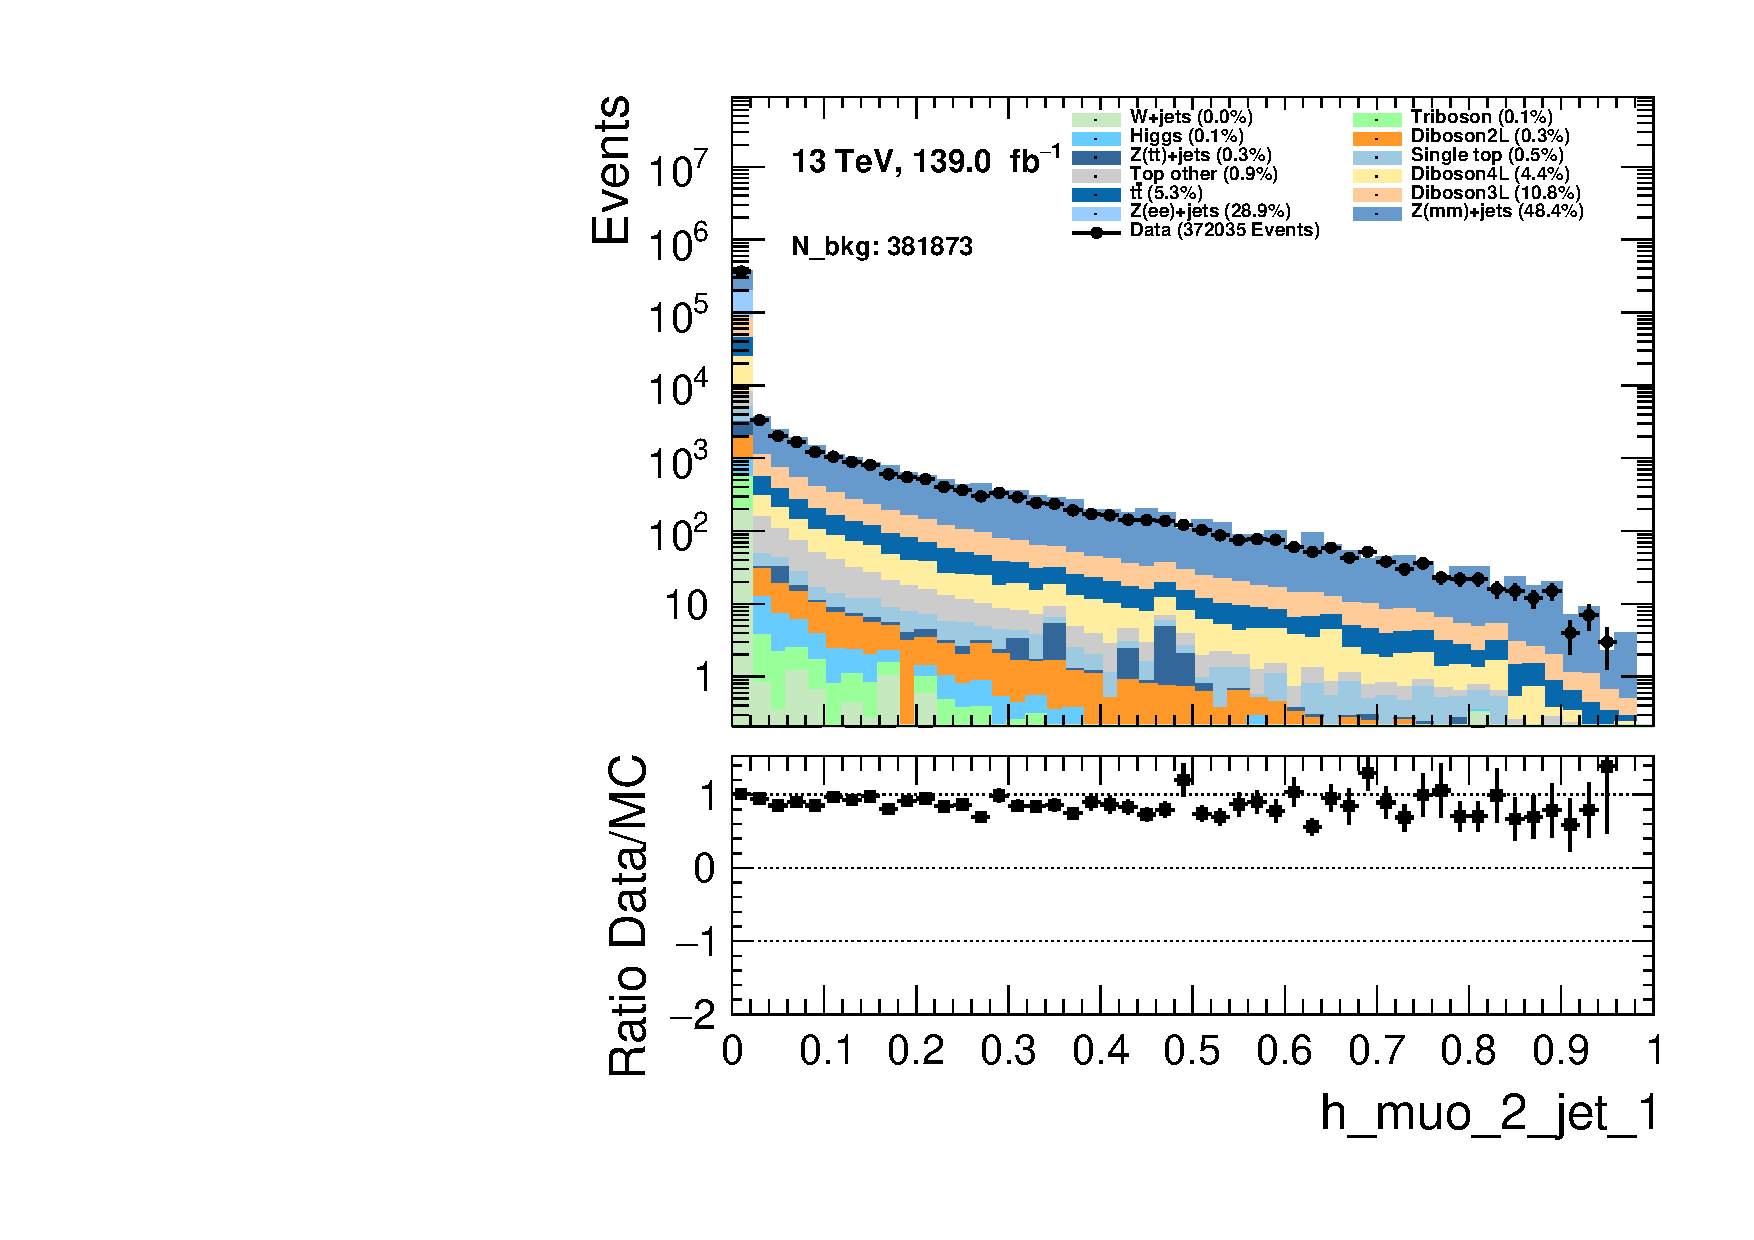
\includegraphics[width=\textwidth]{Figures/MC_Data_comp/h_muo_2_jet_1.pdf}
        \caption{ }
        \label{fig:fe}
    \end{subfigure}
    \hfill       
    \caption{}
    \label{fig:t}
\end{figure}

\begin{figure}
    \centering
    \begin{subfigure}{.49\textwidth}
        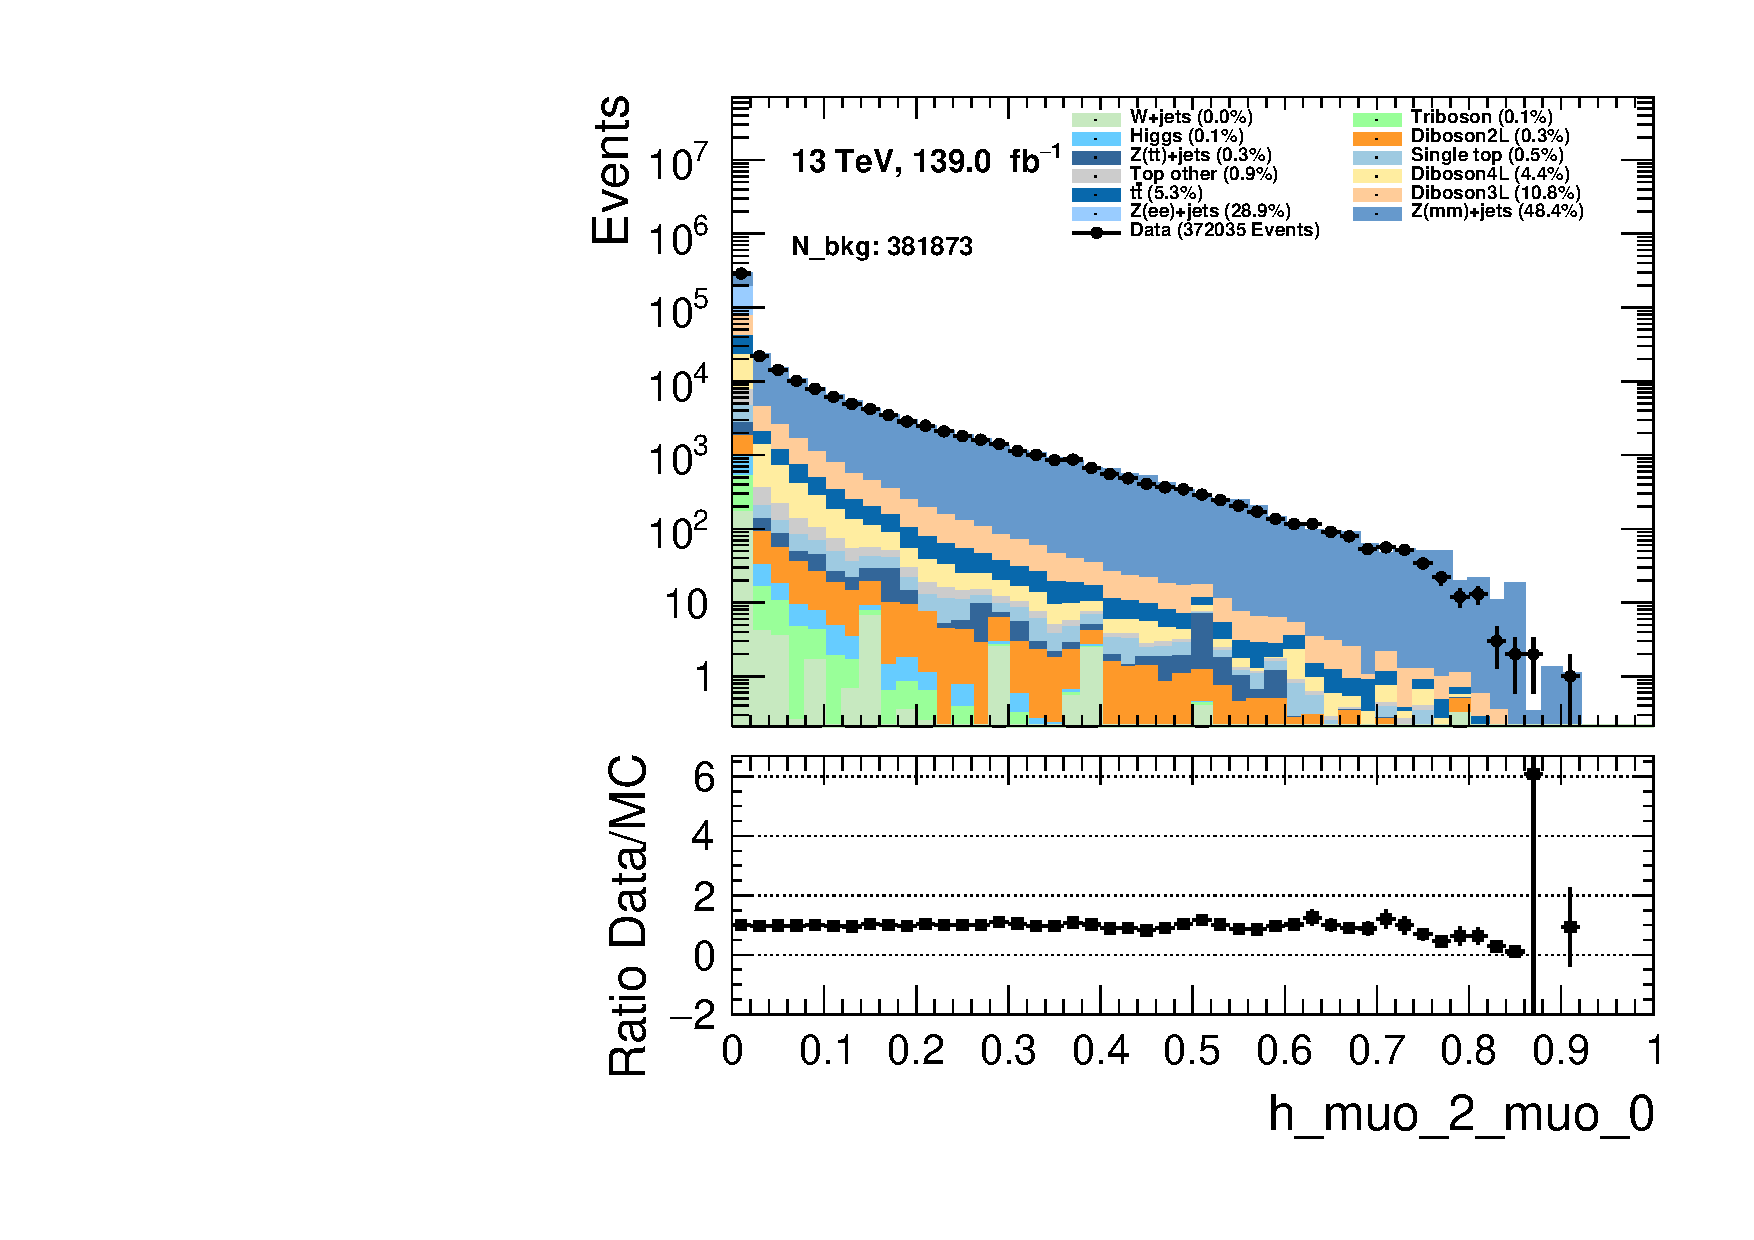
\includegraphics[width=\textwidth]{Figures/MC_Data_comp/h_muo_2_muo_0.pdf}
        \caption{}
        \label{fig:et}
    \end{subfigure}
    \hfill
    \begin{subfigure}{.49\textwidth}
        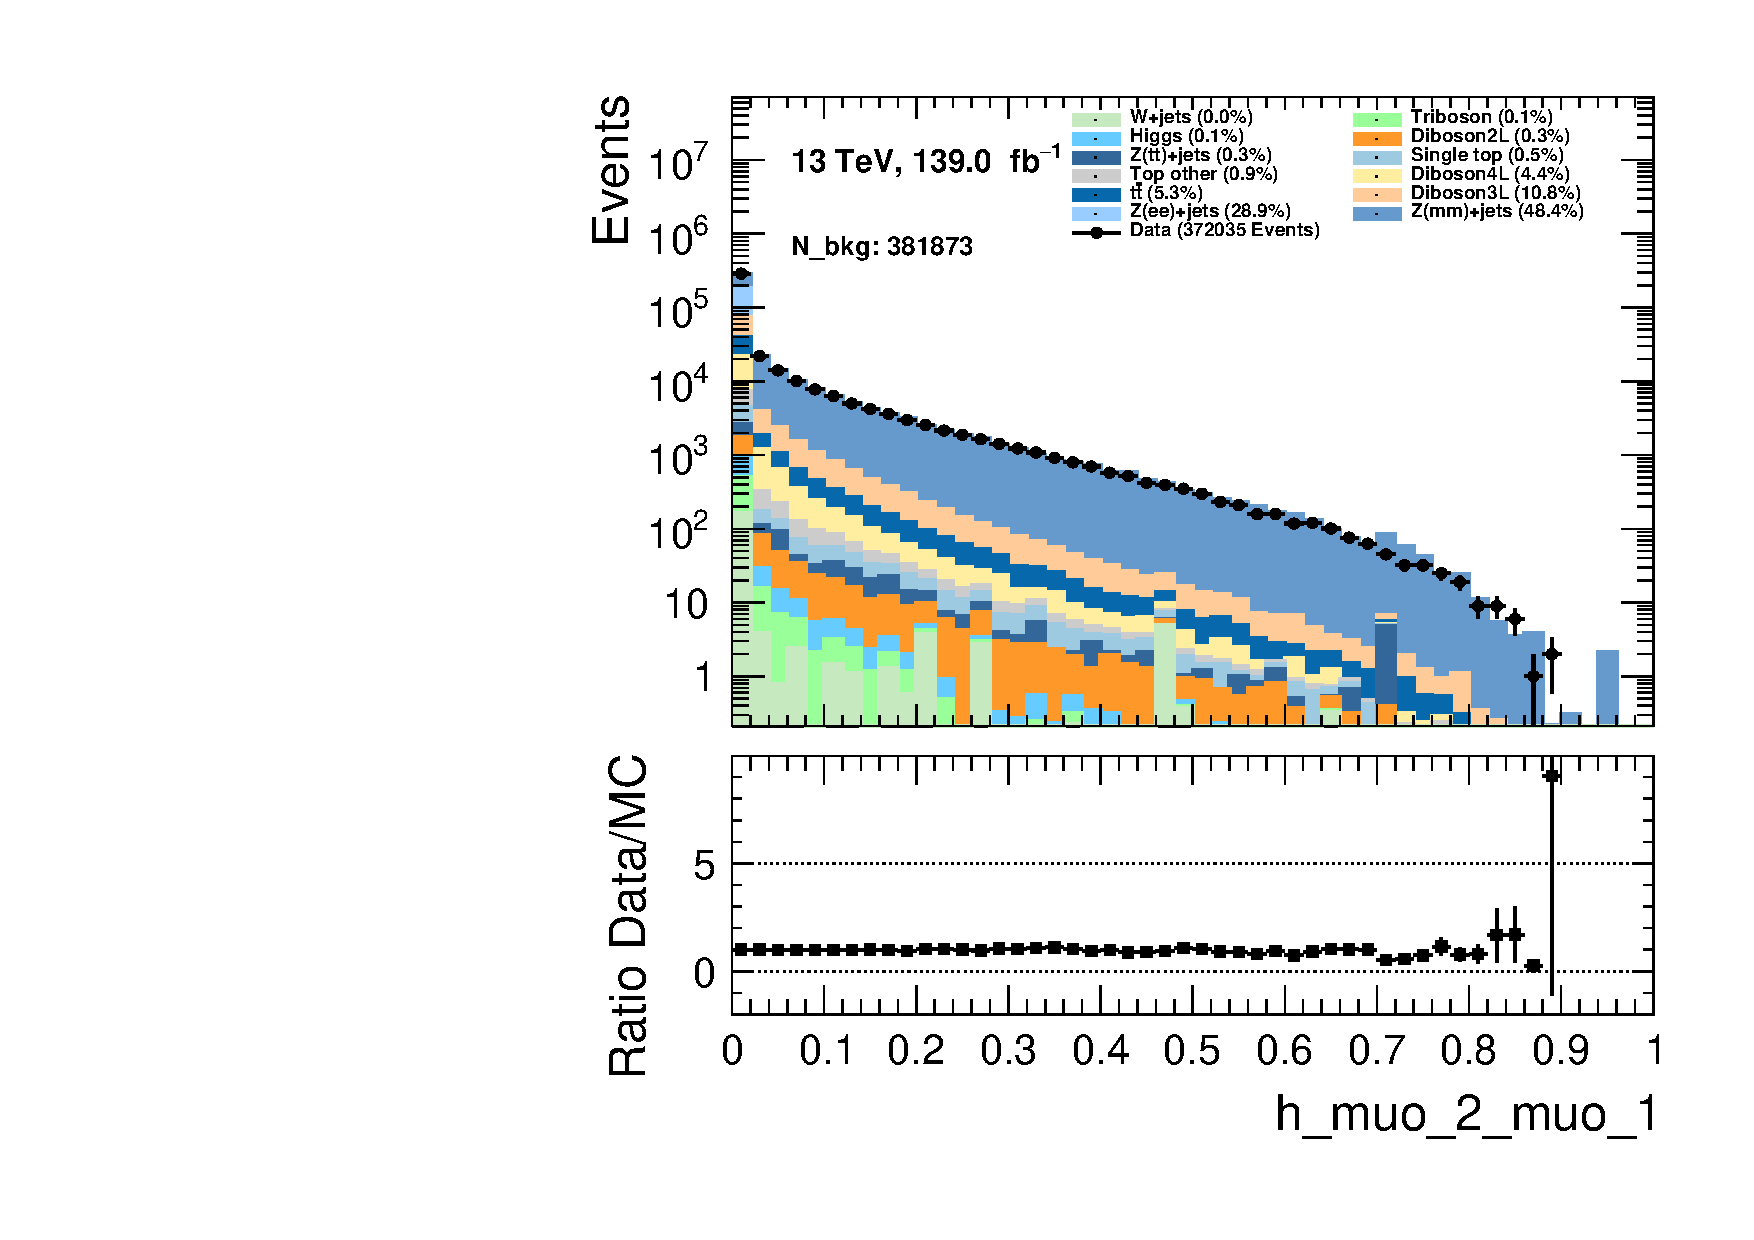
\includegraphics[width=\textwidth]{Figures/MC_Data_comp/h_muo_2_muo_1.pdf}
        \caption{ }
        \label{fig:flcp}
    \end{subfigure}
    \hfill 
    \begin{subfigure}{.49\textwidth}
        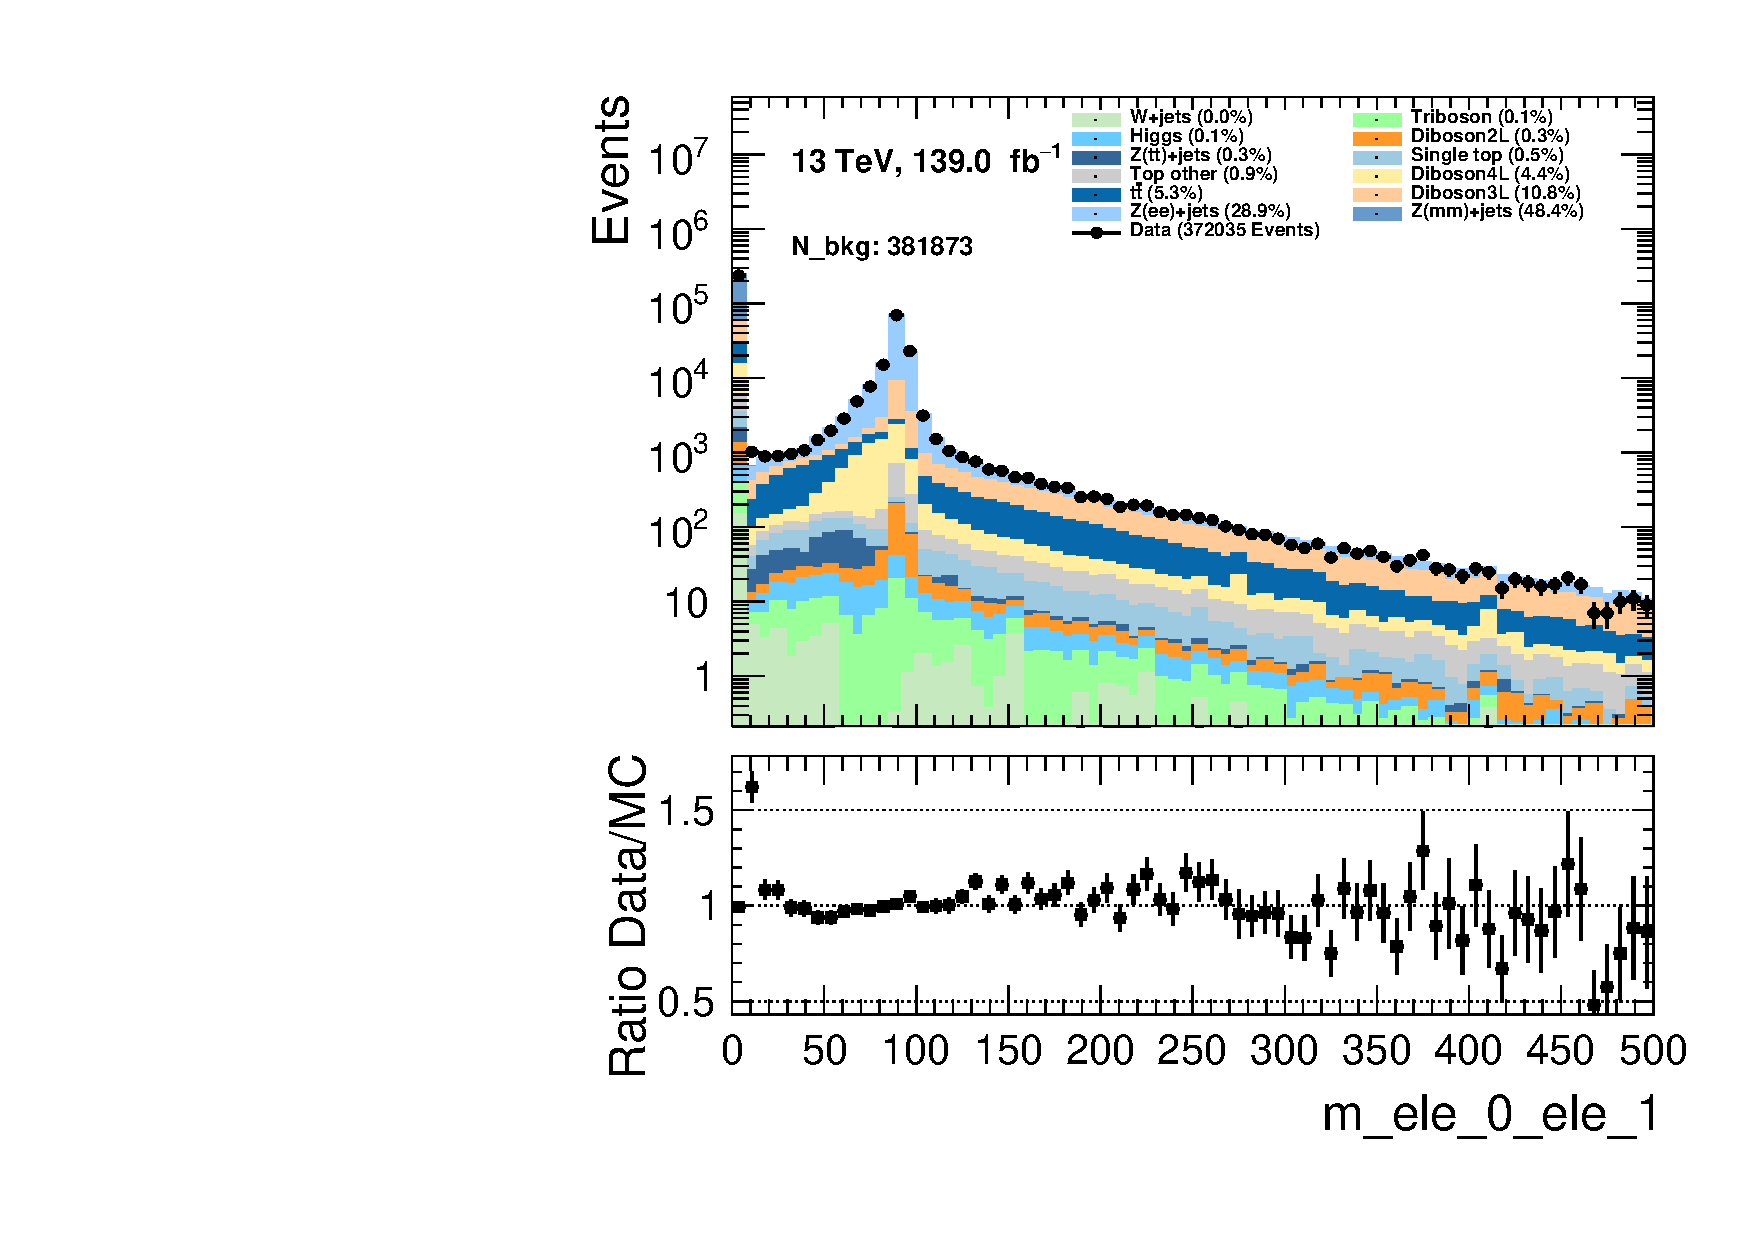
\includegraphics[width=\textwidth]{Figures/MC_Data_comp/m_ele_0_ele_1.pdf}
        \caption{ }
        \label{fig:fep}
    \end{subfigure}
    \hfill
    \begin{subfigure}{.49\textwidth}
        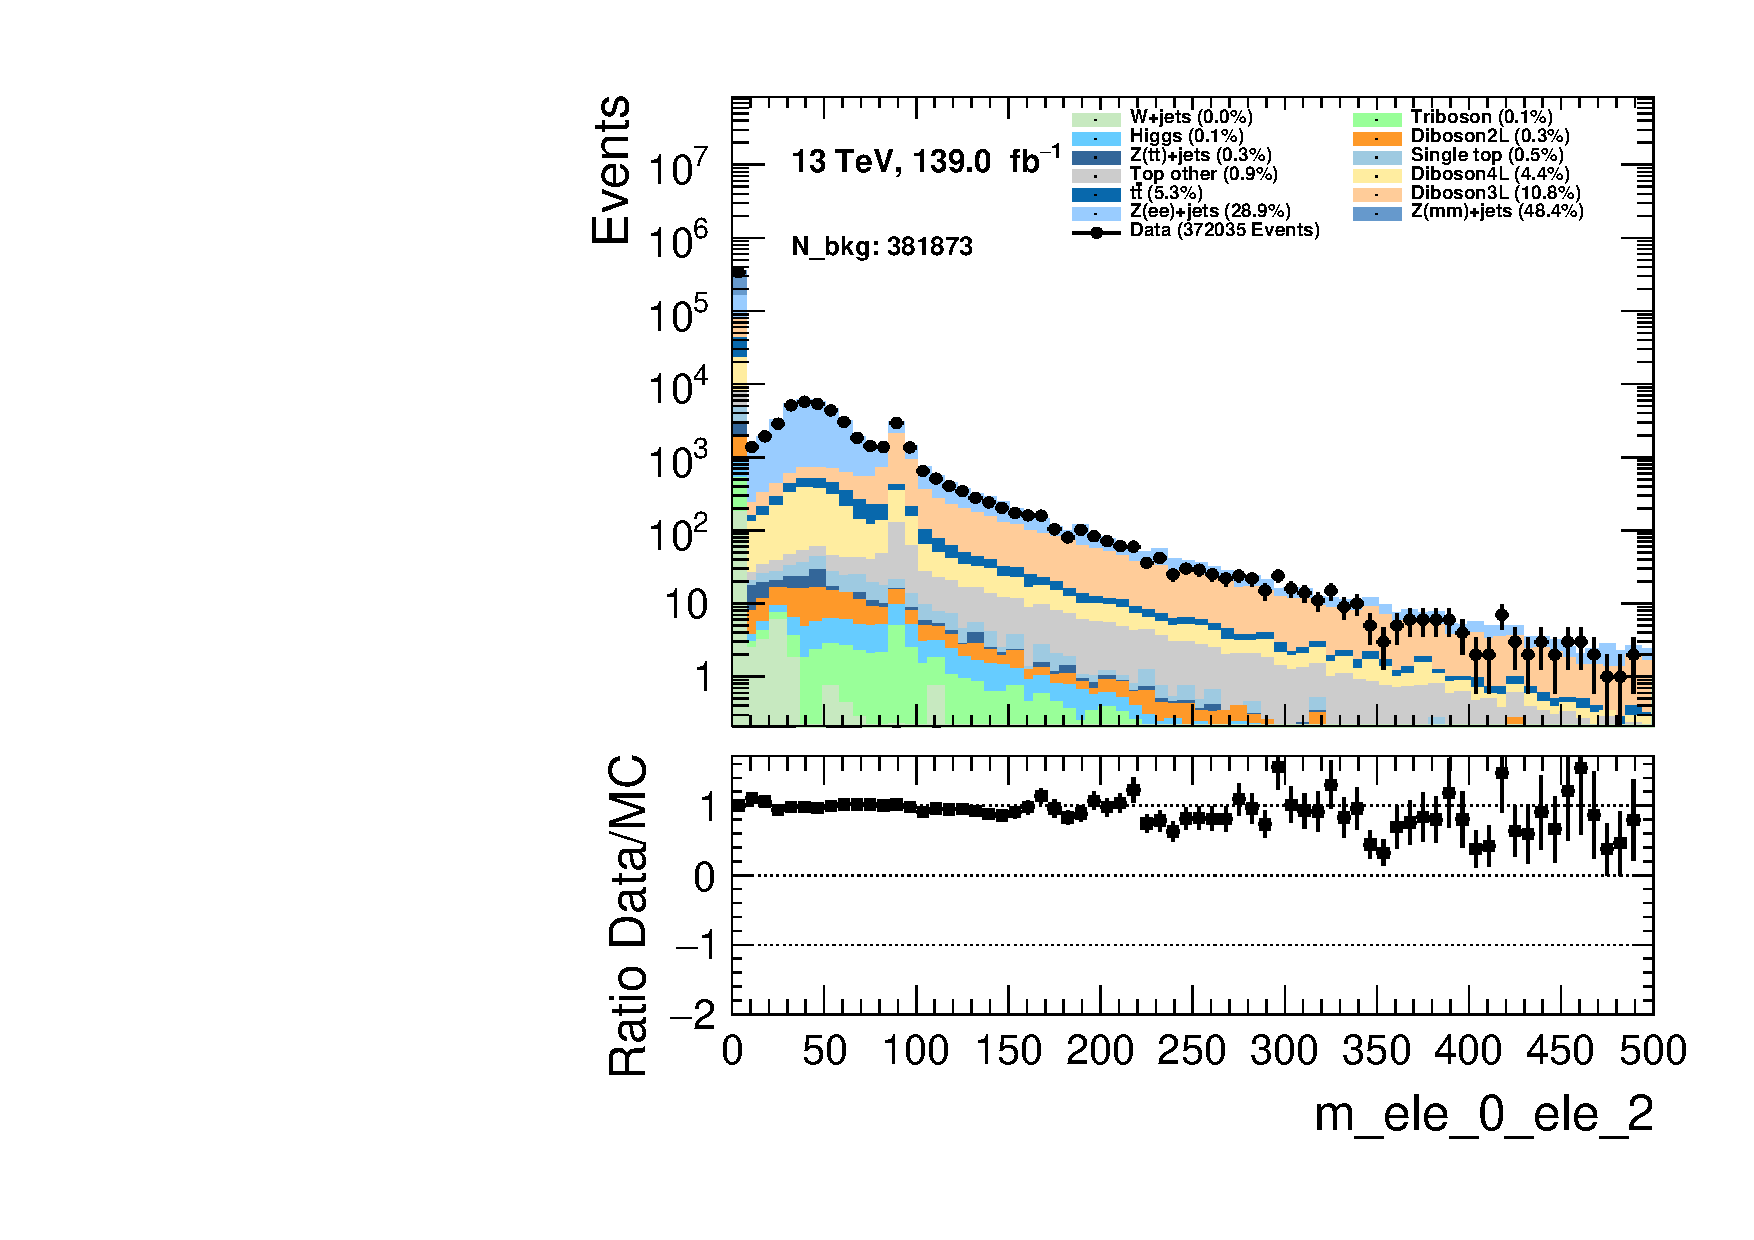
\includegraphics[width=\textwidth]{Figures/MC_Data_comp/m_ele_0_ele_2.pdf}
        \caption{ }
        \label{fig:fe}
    \end{subfigure}
    \hfill       
    \caption{}
    \label{fig:t}
\end{figure}

\begin{figure}
    \centering
    \begin{subfigure}{.49\textwidth}
        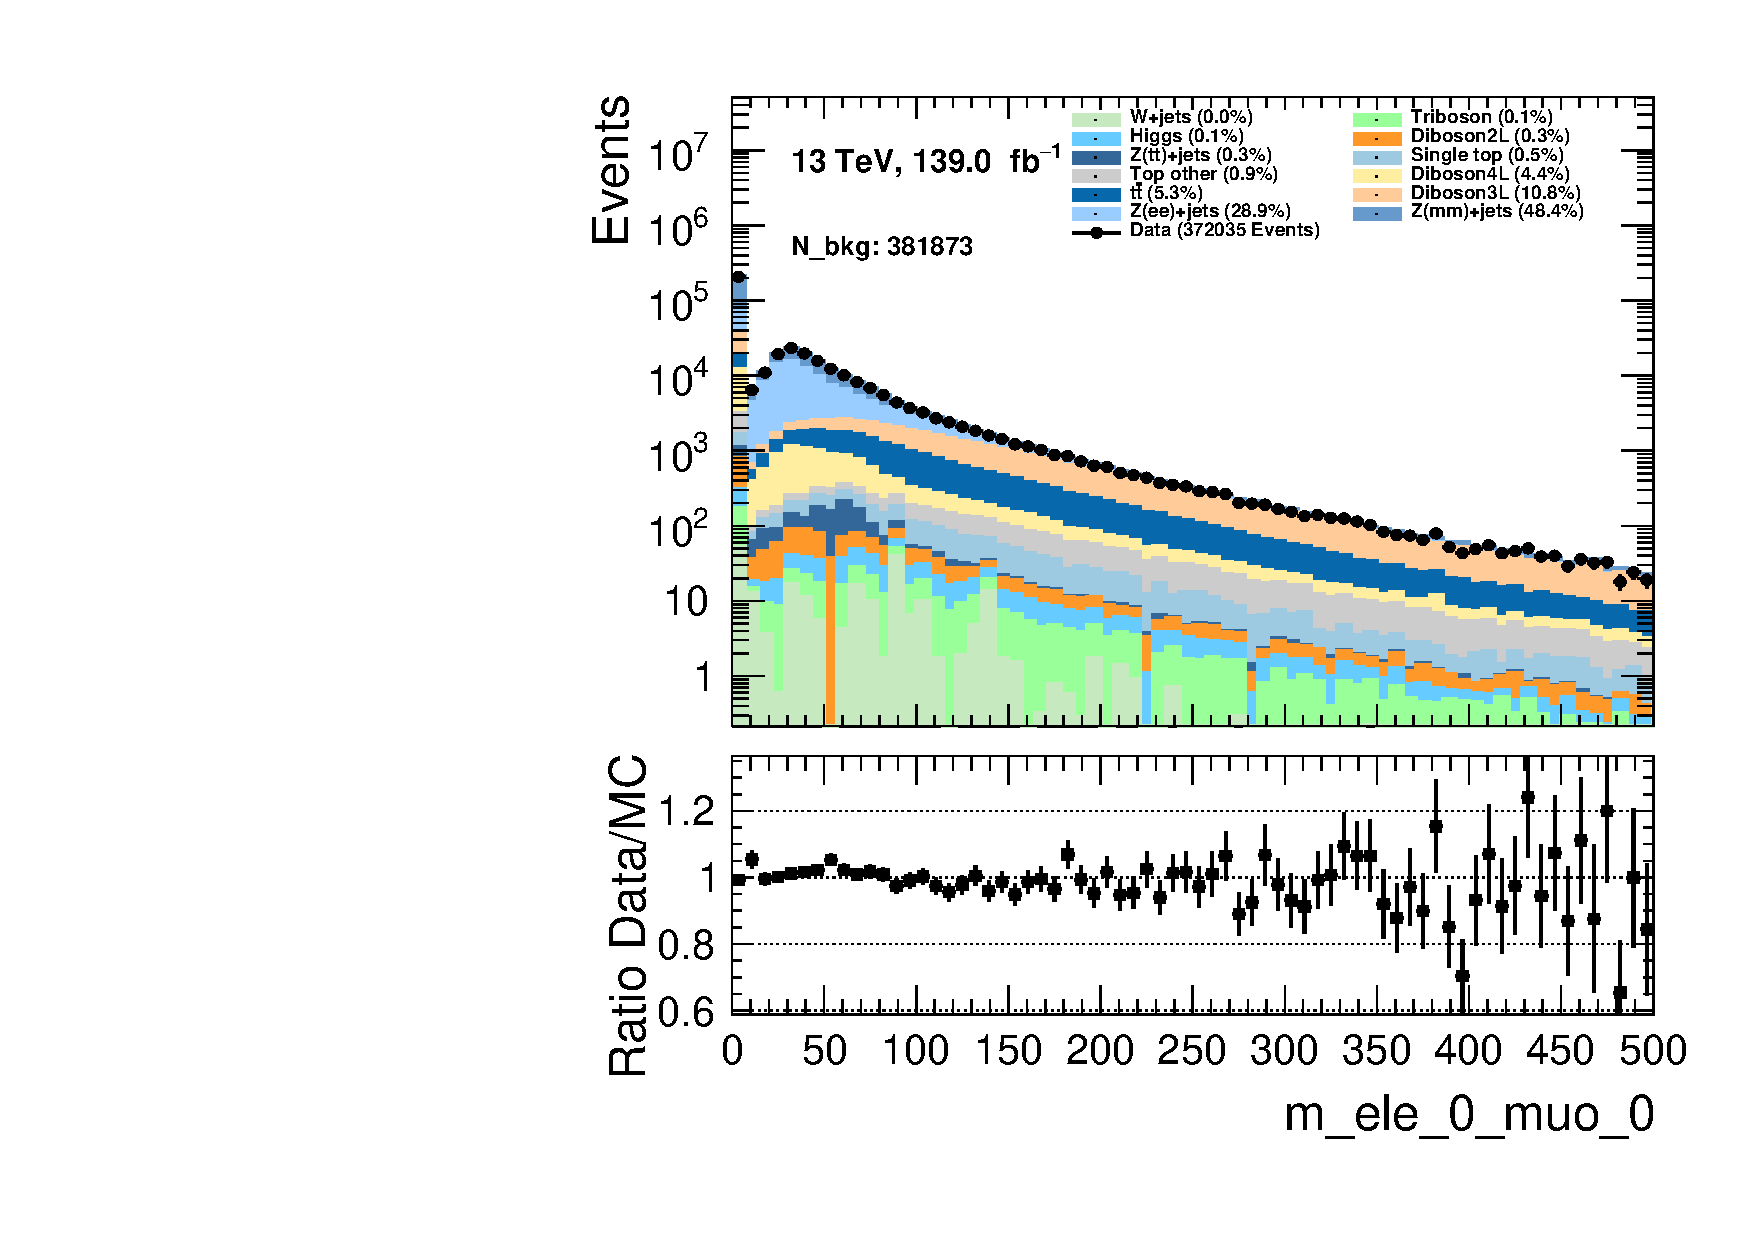
\includegraphics[width=\textwidth]{Figures/MC_Data_comp/m_ele_0_muo_0.pdf}
        \caption{}
        \label{fig:et}
    \end{subfigure}
    \hfill
    \begin{subfigure}{.49\textwidth}
        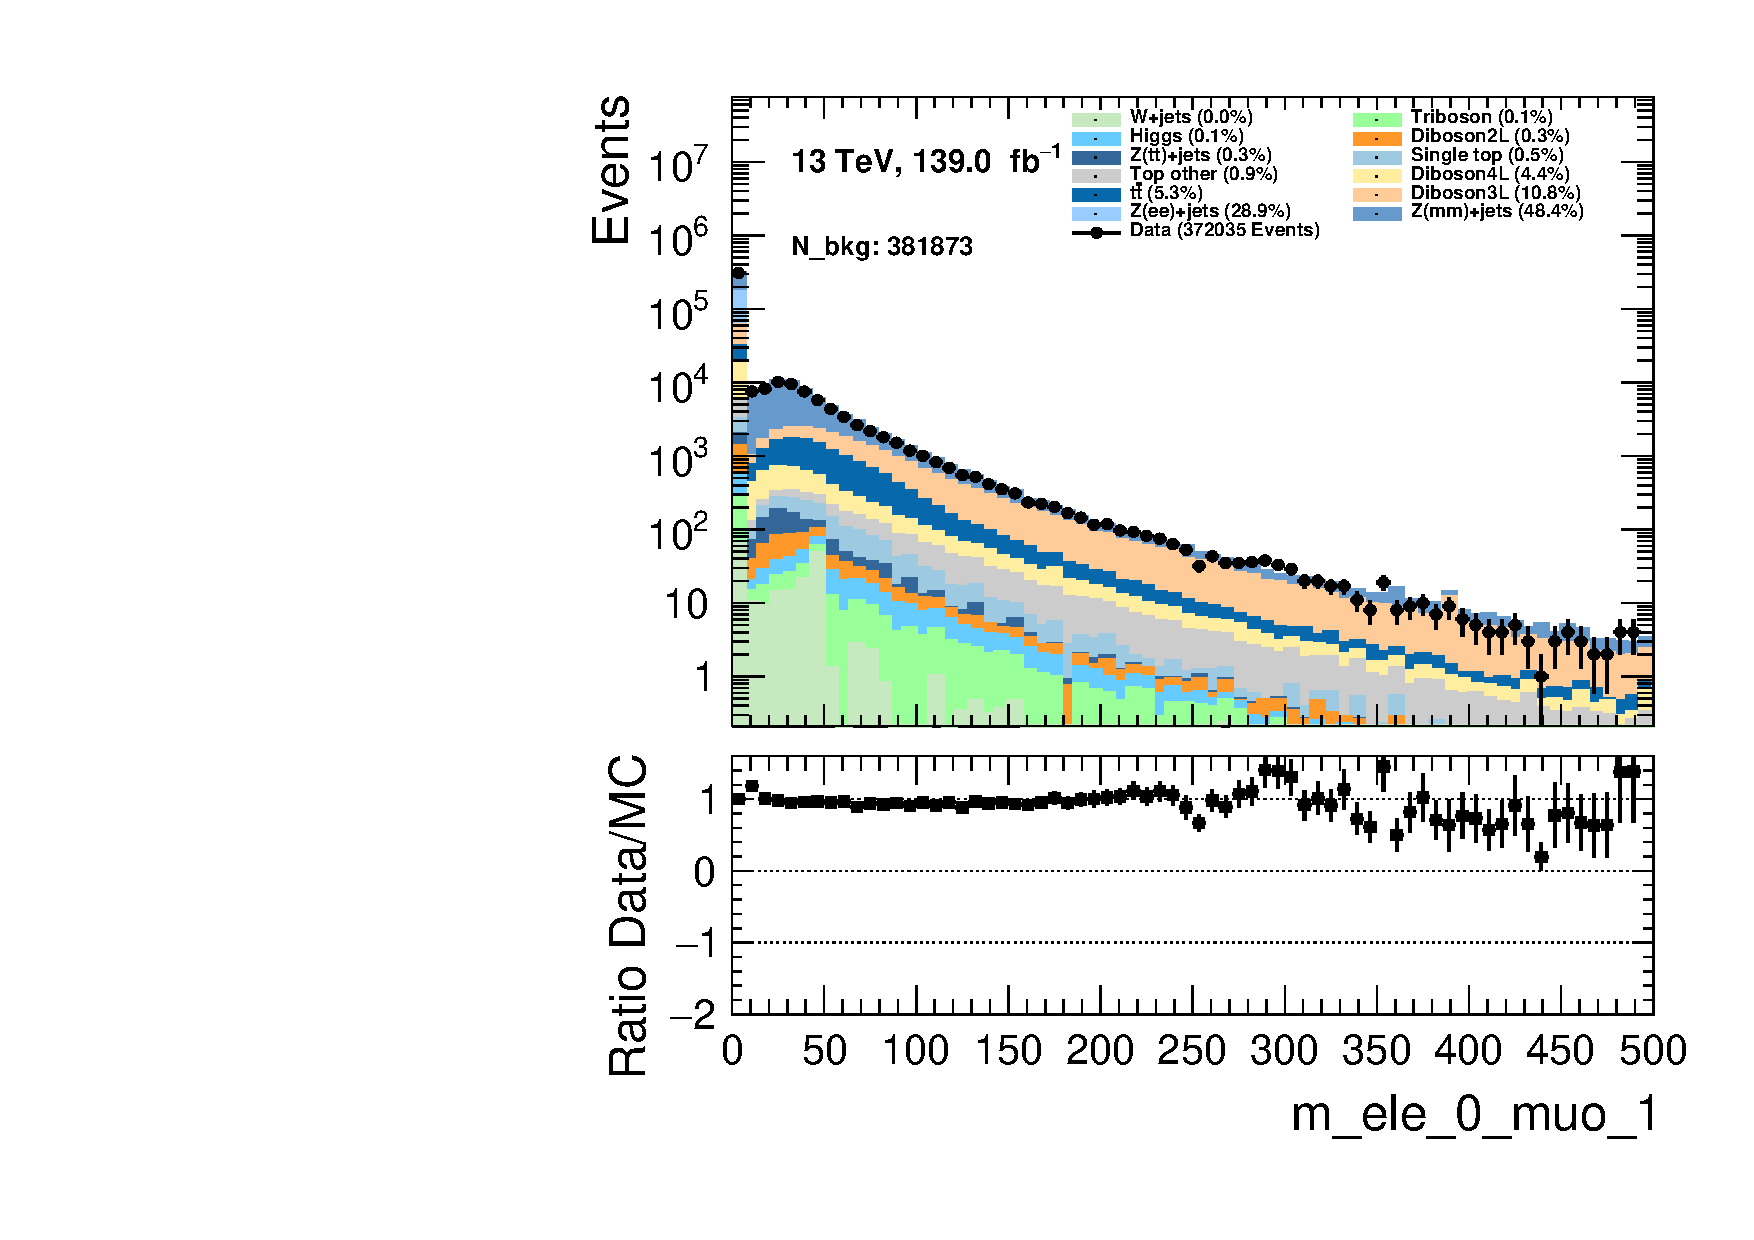
\includegraphics[width=\textwidth]{Figures/MC_Data_comp/m_ele_0_muo_1.pdf}
        \caption{ }
        \label{fig:flcp}
    \end{subfigure}
    \hfill 
    \begin{subfigure}{.49\textwidth}
        \includegraphics[width=\textwidth]{Figures/MC_Data_comp/m_ele_0_muo_2.pdf}
        \caption{ }
        \label{fig:fep}
    \end{subfigure}
    \hfill
    \begin{subfigure}{.49\textwidth}
        \includegraphics[width=\textwidth]{Figures/MC_Data_comp/m_ele_1_ele_2.pdf}
        \caption{ }
        \label{fig:fe}
    \end{subfigure}
    \hfill       
    \caption{}
    \label{fig:t}
\end{figure}

\begin{figure}
    \centering
    \begin{subfigure}{.49\textwidth}
        \includegraphics[width=\textwidth]{Figures/MC_Data_comp/m_ele_1_muo_0.pdf}
        \caption{}
        \label{fig:et}
    \end{subfigure}
    \hfill
    \begin{subfigure}{.49\textwidth}
        \includegraphics[width=\textwidth]{Figures/MC_Data_comp/m_ele_1_muo_1.pdf}
        \caption{ }
        \label{fig:flcp}
    \end{subfigure}
    \hfill 
    \begin{subfigure}{.49\textwidth}
        \includegraphics[width=\textwidth]{Figures/MC_Data_comp/m_ele_1_muo_2.pdf}
        \caption{ }
        \label{fig:fep}
    \end{subfigure}
    \hfill
    \begin{subfigure}{.49\textwidth}
        \includegraphics[width=\textwidth]{Figures/MC_Data_comp/m_ele_2_muo_0.pdf}
        \caption{ }
        \label{fig:fe}
    \end{subfigure}
    \hfill       
    \caption{}
    \label{fig:t}
\end{figure}

\begin{figure}
    \centering
    \begin{subfigure}{.49\textwidth}
        \includegraphics[width=\textwidth]{Figures/MC_Data_comp/m_ele_2_muo_1.pdf}
        \caption{}
        \label{fig:et}
    \end{subfigure}
    \hfill
    \begin{subfigure}{.49\textwidth}
        \includegraphics[width=\textwidth]{Figures/MC_Data_comp/m_ele_2_muo_2.pdf}
        \caption{ }
        \label{fig:flcp}
    \end{subfigure}
    \hfill 
    \begin{subfigure}{.49\textwidth}
        \includegraphics[width=\textwidth]{Figures/MC_Data_comp/m_jet_0_ele_0.pdf}
        \caption{ }
        \label{fig:fep}
    \end{subfigure}
    \hfill
    \begin{subfigure}{.49\textwidth}
        \includegraphics[width=\textwidth]{Figures/MC_Data_comp/m_jet_0_ele_1.pdf}
        \caption{ }
        \label{fig:fe}
    \end{subfigure}
    \hfill       
    \caption{}
    \label{fig:t}
\end{figure}

\begin{figure}
    \centering
    \begin{subfigure}{.49\textwidth}
        \includegraphics[width=\textwidth]{Figures/MC_Data_comp/m_jet_0_ele_2.pdf}
        \caption{}
        \label{fig:et}
    \end{subfigure}
    \hfill
    \begin{subfigure}{.49\textwidth}
        \includegraphics[width=\textwidth]{Figures/MC_Data_comp/m_jet_0_jet_1.pdf}
        \caption{ }
        \label{fig:flcp}
    \end{subfigure}
    \hfill 
    \begin{subfigure}{.49\textwidth}
        \includegraphics[width=\textwidth]{Figures/MC_Data_comp/m_jet_0_muo_0.pdf}
        \caption{ }
        \label{fig:fep}
    \end{subfigure}
    \hfill
    \begin{subfigure}{.49\textwidth}
        \includegraphics[width=\textwidth]{Figures/MC_Data_comp/m_jet_0_muo_1.pdf}
        \caption{ }
        \label{fig:fe}
    \end{subfigure}
    \hfill       
    \caption{}
    \label{fig:t}
\end{figure}

\begin{figure}
    \centering
    \begin{subfigure}{.49\textwidth}
        \includegraphics[width=\textwidth]{Figures/MC_Data_comp/m_jet_1_ele_0.pdf}
        \caption{}
        \label{fig:et}
    \end{subfigure}
    \hfill
    \begin{subfigure}{.49\textwidth}
        \includegraphics[width=\textwidth]{Figures/MC_Data_comp/m_jet_1_ele_1.pdf}
        \caption{ }
        \label{fig:flcp}
    \end{subfigure}
    \hfill 
    \begin{subfigure}{.49\textwidth}
        \includegraphics[width=\textwidth]{Figures/MC_Data_comp/m_jet_1_ele_2.pdf}
        \caption{ }
        \label{fig:fep}
    \end{subfigure}
    \hfill
    \begin{subfigure}{.49\textwidth}
        \includegraphics[width=\textwidth]{Figures/MC_Data_comp/m_jet_1_muo_0.pdf}
        \caption{ }
        \label{fig:fe}
    \end{subfigure}
    \hfill       
    \caption{}
    \label{fig:t}
\end{figure}

\begin{figure}
    \centering
    \begin{subfigure}{.49\textwidth}
        \includegraphics[width=\textwidth]{Figures/MC_Data_comp/m_jet_1_muo_1.pdf}
        \caption{}
        \label{fig:et}
    \end{subfigure}
    \hfill
    \begin{subfigure}{.49\textwidth}
        \includegraphics[width=\textwidth]{Figures/MC_Data_comp/m_jet_1_muo_2.pdf}
        \caption{ }
        \label{fig:flcp}
    \end{subfigure}
    \hfill 
    \begin{subfigure}{.49\textwidth}
        \includegraphics[width=\textwidth]{Figures/MC_Data_comp/m_muo_0_muo_1.pdf}
        \caption{ }
        \label{fig:fep}
    \end{subfigure}
    \hfill
    \begin{subfigure}{.49\textwidth}
        \includegraphics[width=\textwidth]{Figures/MC_Data_comp/m_muo_0_muo_2.pdf}
        \caption{ }
        \label{fig:fe}
    \end{subfigure}
    \hfill       
    \caption{}
    \label{fig:t}
\end{figure}

\begin{figure}
    \centering
    \begin{subfigure}{.49\textwidth}
        \includegraphics[width=\textwidth]{Figures/MC_Data_comp/m_T_ele_0.pdf}
        \caption{}
        \label{fig:et}
    \end{subfigure}
    \hfill
    \begin{subfigure}{.49\textwidth}
        \includegraphics[width=\textwidth]{Figures/MC_Data_comp/m_T_ele_1.pdf}
        \caption{ }
        \label{fig:flcp}
    \end{subfigure}
    \hfill 
    \begin{subfigure}{.49\textwidth}
        \includegraphics[width=\textwidth]{Figures/MC_Data_comp/m_T_ele_2.pdf}
        \caption{ }
        \label{fig:fep}
    \end{subfigure}
    \hfill
    \begin{subfigure}{.49\textwidth}
        \includegraphics[width=\textwidth]{Figures/MC_Data_comp/m_T_jet_0.pdf}
        \caption{ }
        \label{fig:fe}
    \end{subfigure}
    \hfill       
    \caption{}
    \label{fig:t}
\end{figure}


\begin{figure}
    \centering
    \begin{subfigure}{.49\textwidth}
        \includegraphics[width=\textwidth]{Figures/MC_Data_comp/m_T_jet_1.pdf}
        \caption{}
        \label{fig:et}
    \end{subfigure}
    \hfill
    \begin{subfigure}{.49\textwidth}
        \includegraphics[width=\textwidth]{Figures/MC_Data_comp/m_T_muo_0.pdf}
        \caption{ }
        \label{fig:flcp}
    \end{subfigure}
    \hfill 
    \begin{subfigure}{.49\textwidth}
        \includegraphics[width=\textwidth]{Figures/MC_Data_comp/m_T_muo_1.pdf}
        \caption{ }
        \label{fig:fep}
    \end{subfigure}
    \hfill
    \begin{subfigure}{.49\textwidth}
        \includegraphics[width=\textwidth]{Figures/MC_Data_comp/m_T_muo_2.pdf}
        \caption{ }
        \label{fig:fe}
    \end{subfigure}
    \hfill       
    \caption{}
    \label{fig:t}
\end{figure}

\begin{figure}
    \centering
    \begin{subfigure}{.49\textwidth}
        \includegraphics[width=\textwidth]{Figures/MC_Data_comp/muo_0_charge.pdf}
        \caption{}
        \label{fig:et}
    \end{subfigure}
    \hfill
    \begin{subfigure}{.49\textwidth}
        \includegraphics[width=\textwidth]{Figures/MC_Data_comp/muo_1_charge.pdf}
        \caption{ }
        \label{fig:flcp}
    \end{subfigure}
    \hfill 
    \begin{subfigure}{.49\textwidth}
        \includegraphics[width=\textwidth]{Figures/MC_Data_comp/muo_2_charge.pdf}
        \caption{ }
        \label{fig:fep}
    \end{subfigure}
    \hfill
    
         
    \caption{}
    \label{fig:t}
\end{figure}